%\documentclass[compress]{beamer}
\documentclass[8pt,xcolor=dvipnames]{beamer}

%-----------------------------------------------------------
% PACKAGES

%\usepackage[latin1]{inputenc}
\mode<presentation>

%\usepackage[T1]{fontenc}  
%\usetheme{Warsaw}
\usetheme{Frankfurt}
\definecolor{maroon}{RGB}{80, 0.0, 0.0}
\usecolortheme[named=maroon]{structure}
\useoutertheme[subsection=false]{miniframes}
\usepackage{etoolbox}
\makeatletter
\patchcmd{\slideentry}{\advance\beamer@xpos by1\relax}{}{}{}
\def\beamer@subsectionentry#1#2#3#4#5{\advance\beamer@xpos by1\relax}%
\makeatother

%\setbeamercolor{block title}{bg=red!30,fg=black}

\usepackage{graphicx}
%\usepackage[section]{placeins} % force � mettre l'image o� on veut
%\usepackage{float} %utiliser H pour forcer � mettre l'image o� on veut
\usepackage{lscape} %utilisation du mode paysage
%\usepackage{pslatex}
\usepackage{url}
\usepackage{subfigure}

\usepackage{graphicx}
\usepackage{tabls}
\usepackage{afterpage}

\usepackage{ocgx2}
\usepackage[]{media9}
%\usepackage{multimedia}

\usepackage{amsthm}
\usepackage{amssymb}
\usepackage{amsmath}
\usepackage{amsfonts}
\usepackage{amstext}
\usepackage{amsbsy}
\usepackage{mathbbol} 
\usepackage{mathrsfs}

\usepackage{epsfig}
%\usepackage{epsfig}
%\usepackage{cites}
\usepackage{epsf}
\usepackage{array}
\usepackage{color}
\usepackage{pdfpages}
\usepackage{cancel}

\usepackage{tikz}
\usepackage{colortbl}
%\usepackage{booktabs}
\usepackage{multicol}
\usepackage{caption}

%-----------------------------------------------------------
% NEW  DEFINITIONS
%
%=================================================================================================
% new commands
% +++++++++++++++++++++++++++++++++++++++++++++++++++++++++++++++++++++++++++++++++++++++++++++++++
\newcommand{\nc}{\newcommand}
%
% Ways of grouping things
%
\newcommand{\bracket}[1]{\left[ #1 \right]}
\newcommand{\bracet}[1]{\left\{ #1 \right\}}
\newcommand{\fn}[1]{\left( #1 \right)}
\newcommand{\ave}[1]{\left\langle #1 \right\rangle}
%
% Derivative forms
% 
\newcommand{\dx}[1]{\,d#1}
\newcommand{\dxdy}[2]{\frac{\partial #1}{\partial #2}}
\newcommand{\dxdt}[1]{\frac{\partial #1}{\partial t}}
\newcommand{\dxdz}[1]{\frac{\partial #1}{\partial z}}
\newcommand{\dfdt}[1]{\frac{\partial}{\partial t} \fn{#1}}
\newcommand{\dfdz}[1]{\frac{\partial}{\partial z} \fn{#1}}
\newcommand{\ddt}[1]{\frac{\partial}{\partial t} #1}
\newcommand{\ddz}[1]{\frac{\partial}{\partial z} #1}
\newcommand{\dd}[2]{\frac{\partial}{\partial #1} #2}
\newcommand{\ddx}[1]{\frac{\partial}{\partial x} #1}
\newcommand{\ddy}[1]{\frac{\partial}{\partial y} #1}
%
% Vector forms
%
%\renewcommand{\vec}[1]{\ensuremath{\stackrel{\rightarrow}{#1}}}
%\renewcommand{\div}{\ensuremath{\vec{\nabla} \cdot}}
%\newcommand{\grad}{\ensuremath{\vec{\nabla}}}

\renewcommand{\div}{\vec{\nabla}\! \cdot \!}
\newcommand{\grad}{\vec{\nabla}}
\newcommand{\oa}[1]{\fn{\frac{1}{3}\hat{\Omega}\!\cdot\!\overrightarrow{A_{#1}}}}

%
% Equation beginnings and endings
%
\newcommand{\bea}{\begin{eqnarray}}
\newcommand{\eea}{\end{eqnarray}}
\newcommand{\be}{\begin{equation*}}
\newcommand{\ee}{\end{equation*}}
\newcommand{\beas}{\begin{eqnarray*}}
\newcommand{\eeas}{\end{eqnarray*}}
\newcommand{\bdm}{\begin{displaymath}}
\newcommand{\edm}{\end{displaymath}}
%
% Equation punctuation
% 
\newcommand{\pec}{\hspace{0.25in},}
\newcommand{\pep}{\hspace{0.25in}.}
\newcommand{\pev}{\hspace{0.25in}}
%
% Equation labels and references, figure references, table references
% 
\newcommand{\LEQ}[1]{\label{eq:#1}}
\newcommand{\EQ}[1]{Eq.~(\ref{eq:#1})}
\newcommand{\EQS}[1]{Eqs.~(\ref{eq:#1})}
\newcommand{\REQ}[1]{\ref{eq:#1}}
\newcommand{\LFI}[1]{\label{fi:#1}}
\newcommand{\FI}[1]{Fig.~\ref{fi:#1}}
\newcommand{\RFI}[1]{\ref{fi:#1}}
\newcommand{\LTA}[1]{\label{ta:#1}}
\newcommand{\TA}[1]{Table~\ref{ta:#1}}
\newcommand{\RTA}[1]{\ref{ta:#1}}

%
% List beginnings and endings
% 
\newcommand{\bl}{\bss\begin{itemize}}
\newcommand{\el}{\vspace{-.5\baselineskip}\end{itemize}\ess}
\newcommand{\benu}{\bss\begin{enumerate}}
\newcommand{\eenu}{\vspace{-.5\baselineskip}\end{enumerate}\ess}
%
% Figure and table beginnings and endings
% 
\newcommand{\bfg}{\begin{figure}}
\newcommand{\efg}{\end{figure}}
\newcommand{\bt}{\begin{table}}
\newcommand{\et}{\end{table}}
%
% Tabular and center beginnings and endings
% 
\newcommand{\bc}{\begin{center}}
\newcommand{\ec}{\end{center}}
\newcommand{\btb}{\begin{center}\begin{tabular}}
\newcommand{\etb}{\end{tabular}\end{center}}
%
% Single space command
% 
%\newcommand{\bss}{\begin{singlespace}}
%\newcommand{\ess}{\end{singlespace}}
\newcommand{\bss}{\singlespacing}
\newcommand{\ess}{\doublespacing}
%
%---New environment "arbspace". (modeled after singlespace environment
%                                in Doublespace.sty)
%   The baselinestretch only takes effect at a size change, so do one.
% 
\def\arbspace#1{\def\baselinestretch{#1}\@normalsize}
\def\endarbspace{}
\newcommand{\bas}{\begin{arbspace}}
\newcommand{\eas}{\end{arbspace}}
%
% An explanation for a function
%
\newcommand{\explain}[1]{\mbox{\hspace{2em} #1}}
%
% Quick commands for symbols
%  
\newcommand{\half}{\frac{1}{2}}
\newcommand{\third}{\frac{1}{3}}
\newcommand{\twothird}{\frac{2}{3}}
\newcommand{\fourth}{\frac{1}{4}}
\newcommand{\mdot}{\dot{m}}
\newcommand{\ten}[1]{\times 10^{#1}\,}
\newcommand{\cL}{{\cal L}}
\newcommand{\cD}{{\cal D}}
\newcommand{\cF}{{\cal F}}
\newcommand{\cE}{{\cal E}}
\renewcommand{\Re}{\mbox{Re}}
\newcommand{\Ma}{\mbox{Ma}}
%
% Inclusion of Graphics Data
%
%\input{psfig}
%\psfiginit
%
% More Quick Commands
% 
\newcommand{\bi}{\begin{itemize}}
\newcommand{\ei}{\end{itemize}}
\newcommand{\ben}{\begin{enumerate}}
\newcommand{\een}{\end{enumerate}}
\newcommand{\dxi}{\Delta x_i}
\newcommand{\dyj}{\Delta y_j}
\newcommand{\ts}[1]{\textstyle #1}


\newcommand{\bu}{\boldsymbol{u}}
\newcommand{\ber}{\boldsymbol{e}}
\newcommand{\br}{\boldsymbol{r}} 
\newcommand{\bo}{\boldsymbol{\Omega}}

\newcommand{\bn}{\boldsymbol{\nabla}}

% DGFEM commands
\newcommand{\jmp}[1]{[\![#1]\!]}                     % jump
\newcommand{\mvl}[1]{\{\!\!\{#1\}\!\!\}}             % mean value


\newcommand{\boxedeqn}[1]{%
  \[\fbox{%
      \addtolength{\linewidth}{-2\fboxsep}%
      \addtolength{\linewidth}{-2\fboxrule}%
      \begin{minipage}{\linewidth}%
      \begin{equation}#1\end{equation}%
      \end{minipage}%
    }\]%
}
\newcommand{\mboxed}[1]{\boxed{\phantom{#1}}}
\newcommand{\ud}{\,\mathrm{d}}

% keff
\newcommand{\keff}{\ensuremath{k_{\textit{eff}}}}

% shortcut for domain notation
\newcommand{\D}{\mathcal{D}}

% vector shortcuts
\newcommand{\vo}{\vec{\Omega}}
\newcommand{\vr}{\vec{r}}
\newcommand{\vn}{\vec{n}}
\newcommand{\vnk}{\vec{\mathbf{n}}}

% extra space
\newcommand{\qq}{\quad\quad}

% common reference commands
\newcommand{\eqt}[1]{Eq.~(\ref{#1})}                     % equation
\newcommand{\fig}[1]{Fig.~\ref{#1}}                      % figure
\newcommand{\tbl}[1]{Table~\ref{#1}}                     % table


\newcommand{\bs}[1]{\mathbf{#1}}
\renewcommand{\bs}[1]{\vec{#1}}
%\newcommand{\dd}{\mathrm{d}}
\newcommand{\norm}[1]{\left\lVert#1\right\rVert_{L^2}}

\newcommand{\divv}[1]{\vec{\nabla}^{#1}\! \cdot \!}
\newcommand{\gradd}[1]{\vec{\nabla}^{#1}}

\definecolor{britishracinggreen}{rgb}{0.0, 0.26, 0.15}
\newcommand{\tcr}[1]{\textcolor{red}{#1}}
\newcommand{\tcb}[1]{\textcolor{blue}{#1}}
\newcommand{\tcm}[1]{\textcolor{magenta}{#1}}
\newcommand{\tcp}[1]{\textcolor{violet}{#1}}
\newcommand{\tcg}[1]{\textcolor{britishracinggreen}{#1}}

\renewcommand{\L}{\mathbf{L}}
\renewcommand{\S}{\mathbf{\Sigma}}
\newcommand{\M}{\mathbf{M}}
\renewcommand{\D}{\mathbf{D}}

\newcommand{\backupbegin}{
   \newcounter{finalframe}
   \setcounter{finalframe}{\value{framenumber}}
}
\newcommand{\backupend}{
   \setcounter{framenumber}{\value{finalframe}}
}

% tikz stuff
\usetikzlibrary{shapes,arrows,positioning}
\pgfdeclarelayer{background}
\pgfdeclarelayer{foreground}
\pgfsetlayers{background,main,foreground}
\tikzstyle{redblock}=[rectangle, draw, align=center, top color=red!25, bottom color=red!75,  minimum width=10mm, minimum height=10mm,]
\tikzstyle{blueblock}=[rectangle,draw, align=center, top color=blue!25, bottom color=blue!75,  minimum width=10mm, minimum height=10mm]
\tikzstyle{purpleblock}=[rectangle,  draw, align=center, top color=purple!25, bottom color=purple!75, minimum width=10mm, minimum height=10mm]
\tikzstyle{orangeblock}=[rectangle, draw, align=center, top color=orange!25, bottom color=orange!75,  minimum width=10mm, minimum height=10mm]
\tikzstyle{greendiamond}=[diamond, draw, align=center, top color=green!25, bottom color=green!75,  minimum width=8mm, aspect=2]
\tikzstyle{greenblock}=[rectangle, rounded corners, draw, align=center, top color=white, bottom color=green!20, ultra thick, minimum width=60mm, minimum height=15mm,]
\tikzstyle{blueblock2}=[rectangle, rounded corners, draw, align=center, top color=white, bottom color=blue!20, ultra thick, minimum width=60mm, minimum height=15mm]
\tikzstyle{reddiamond}=[diamond, draw, align=center, top color=white, bottom color=red!20, ultra thick, minimum width=60mm, aspect=2]
\newcommand{\tikzback}[5]{
 \begin{pgfonlayer}{background}
  \path (#1.west |- #2.north)+(-0.5,0.75) node (a1) {};
  \path (#3.east |- #4.south)+(+0.5,-0.25) node (a2) {};
  \path[fill=yellow!10,rounded corners, draw=black!100, dashed] (a1) rectangle (a2);
   \path (#3.east |- #2.north)+(0,1.25)--(#1.west |- #2.north) node[midway] (#5-n) {};
   \path (#3.east |- #2.south)+(0,-0.35)--(#1.west |- #2.south) node[midway] (#5-s) {};
   \path (#1.west |- #2.north)+(-0.75,0)--(#1.west |- #4.south) node[midway] (#5-w) {};
 \end{pgfonlayer}}

%=================================================================================================

%============================================================

%style et couleur
%\usetheme{Frankfurt}
\date{\today}

%\addtobeamertemplate{footline}{\hfill\insertframenumber/\inserttotalframenumber\hspace{2em}\null}

\setbeamertemplate{footline}{
\leavevmode%
%\hbox{\hspace*{-0.06cm}
\begin{beamercolorbox}[wd=.5\paperwidth,ht=3.25ex,dp=1ex,center]{author in head/foot}%
	\usebeamerfont{author in head/foot}\insertshortauthor%~~(\insertshortinstitute)
\end{beamercolorbox}%
\begin{beamercolorbox}[wd=.25\paperwidth,ht=3.25ex,dp=1ex,center]{section in head/foot}%
	\usebeamerfont{section in head/foot} Final Exam March 2017 % \insertshorttitle
\end{beamercolorbox}%
\begin{beamercolorbox}[wd=.25\paperwidth,ht=3.25ex,dp=1ex,left]{section in head/foot}%
	\usebeamerfont{section in head/foot}\insertshortdate{}\hspace*{2em}
	\insertframenumber{} / \inserttotalframenumber %\hspace*{2ex}
\end{beamercolorbox}}%
%\vskip0pt%
%}

\beamertemplatetransparentcovered

\urldef{\prince}\url{zachmprince@tamu.edu}

\title{Improved Quasi-Static Methods for Time-Dependent Neutron Diffusion and Implementation in Rattlesnake}

\author[Zachary M. Prince]{\Large Zachary M. Prince \\ \vspace{5mm} \normalsize \underline{Committee} \\ Dr. Jean Ragusa (Chair) \\ Dr. Jim Morel \\ Dr. Bojan Popov}
\institute{Final Examination for Partial Fulfillment of a Masters of Science \\ Department of Nuclear Engineering, Texas A\&M University, College Station, TX}

\logo{\includegraphics[height=0.8cm]{figures/TAM-logo.png}}

%%%%%%%%%%%%%%%%%%%%%%%%%%%%%%%%%%%%%%%%%%%%%%%%%%%%%%%%%%%%%%%%%%%%

%%%%%%%%%%%%%%%%%%%%%%%%%%%%%%%%%%%%%%%%%%%%%%%%%%%%%%%%%%%%%%%%%%%%
%%%%%%%%%%%%%%%%%%%%%%%%%%%%%%%%%%%%%%%%%%%%%%%%%%%%%%%%%%%%%%%%%%%%
\begin{document}
%%%%%%%%%%%%%%%%%%%%%%%%%%%%%%%%%%%%%%%%%%%%%%%%%%%%%%%%%%%%%%%%%%%%
%%%%%%%%%%%%%%%%%%%%%%%%%%%%%%%%%%%%%%%%%%%%%%%%%%%%%%%%%%%%%%%%%%%%

%-------------------------------------------------------------------
\begin{frame}

\titlepage
\small{email: {\prince} }

\end{frame}
%-------------------------------------------------------------------

%-------------------------------------------------------------------
\begin{frame}{Objective}

\begin{block}{Purpose Statement}
Investigate and develop the improved quasi-static method (IQS) for minimizing computation expense in transient reactor simulations, while maintaining accuracy.
\end{block}

\begin{block}{What is IQS?}
\begin{itemize}
\item Transient neutronics method meant to minimize expensive diffusion evaluations
\item Non-approximately separates spatial variance and temporal power
\item Impetus is spatial variance doesn't change much in time, compared to powerb
\end{itemize}
\end{block}

\begin{block}{Objectives}
\begin{itemize}
\item Establish IQS performance for various nonlinear iteration techniques applied to transient neutronics
\item Validate time step convergence in transient neutronics problems for IQS with high order discretization schemes
\item Apply IQS to multiphysics simulations
\end{itemize}
\end{block}

%\begin{block}{Conclusions}
%\begin{itemize}
%\item IQS is an effective method for reducing computational expense of transient reactor simulations
%\item The IQS uniqueness criteria is important to keep consistent through nonlinear iteration and accurate precursor evaluation
%\item IQS demonstrates proper error convergence up through fourth order methods and shows impressive performance with time adaptation
%\item IQS implementation in Rattlesnake was effective and greatly reduced computational expense in TREAT simulations
%\end{itemize}
%\end{block}


\end{frame}
%-------------------------------------------------------------------

%-------------------------------------------------------------------
\begin{frame}{Outline}
\begin{multicols}{2}
\tableofcontents 
\end{multicols}
\end{frame}
%-------------------------------------------------------------------

%%%%%%%%%%%%%%%%%%%%%%%%%%%%%%%%%%%%%%%%%%%%%%%%%%%%%%%%%%%%%%%%%%%%
\section{Purpose}
%%%%%%%%%%%%%%%%%%%%%%%%%%%%%%%%%%%%%%%%%%%%%%%%%%%%%%%%%%%%%%%%%%%%

%------------------------------------------------------------------%
\subsection{Background on Transient Reactor Testing}
%------------------------------------------------------------------%

%-------------------------------------------------------------------
\begin{frame}{Transient Testing}

\begin{block}{}
\begin{itemize}
\item Fukushima sparked a systematic demand for accident tolerant reactor system designs
\item New designs are significantly different and require experimental testing 
\item Tesing requires specialized facilities like ACRR at SNL and TREAT at INL
\end{itemize}
\end{block}

\begin{figure}
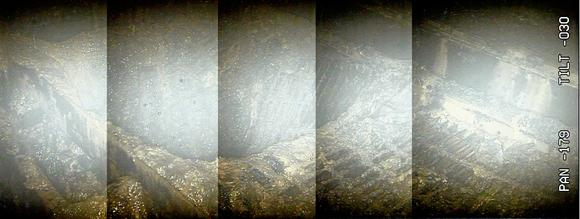
\includegraphics[height=1.5in]{figures/fukushima_melt.jpg}
\caption{Hole believed to be caused by fuel leaking out of the pressure vessel at Fukushima Daiichi nuclear power plant}
\end{figure}

\end{frame}
%-------------------------------------------------------------------

%-------------------------------------------------------------------
\begin{frame}{Transient Reactor Testing Facility (TREAT)}

\begin{figure}
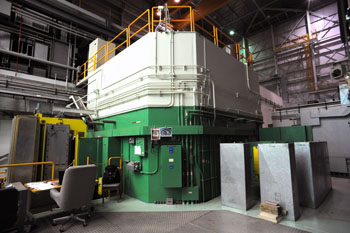
\includegraphics[height=1.5in]{figures/TREAT_outside.jpg}
\hspace{0.1in}
\includegraphics[height=1.5in]{figures/TREAT_core_view.png}
\end{figure}

\begin{block}{}
\begin{itemize}
\item Operation started in 1959, stand-by status in 1994, expected restart by 2020
\item Designed to induce accident-like scenarios to fuel and other reactor components 
\item Air-cooled, graphite moderated, 100 kW steady-state, up to 19 GW peak transients
\end{itemize}
\end{block}

\end{frame}
%-------------------------------------------------------------------

%-------------------------------------------------------------------
\begin{frame}{TREAT Experiments}

\begin{figure}
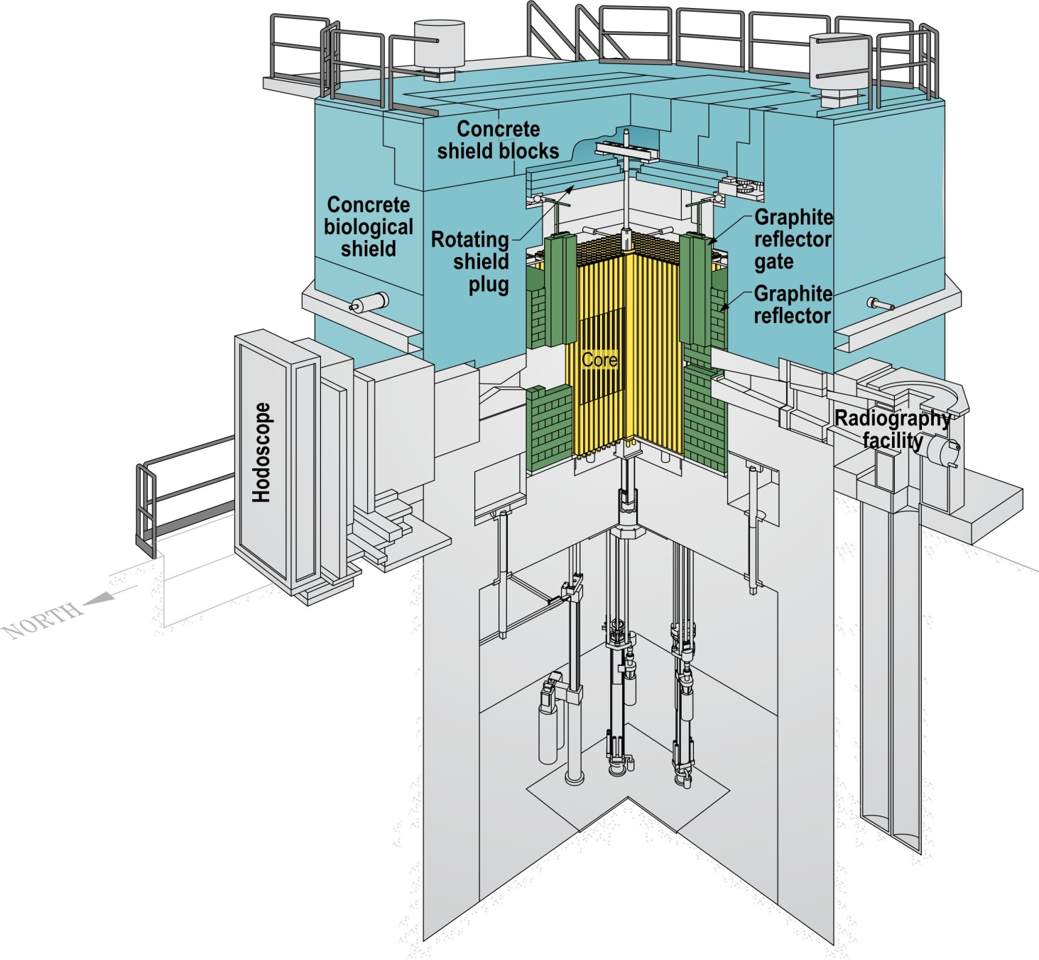
\includegraphics[height=1.75in]{figures/Treat_cutaway.png}
\hspace{0.5in}
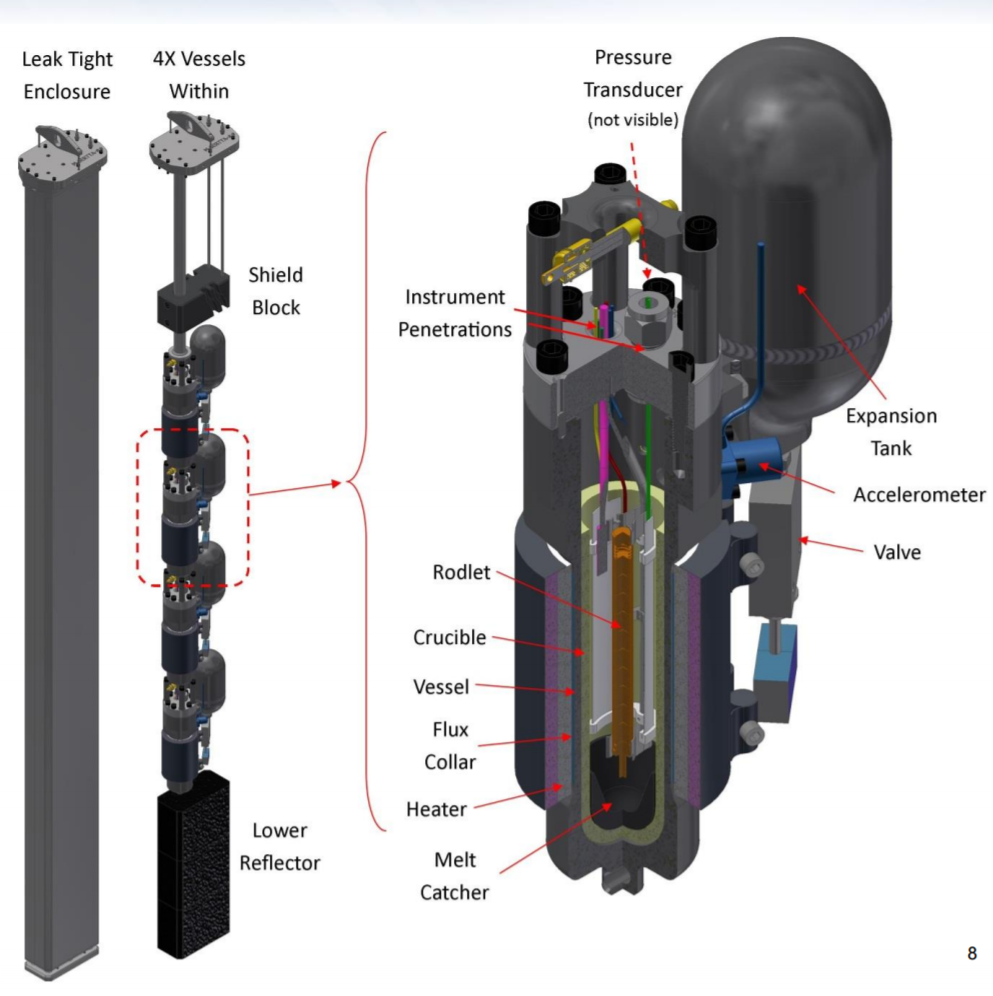
\includegraphics[height=1.75in]{figures/multi_sertta.png}
\end{figure}

\begin{figure}
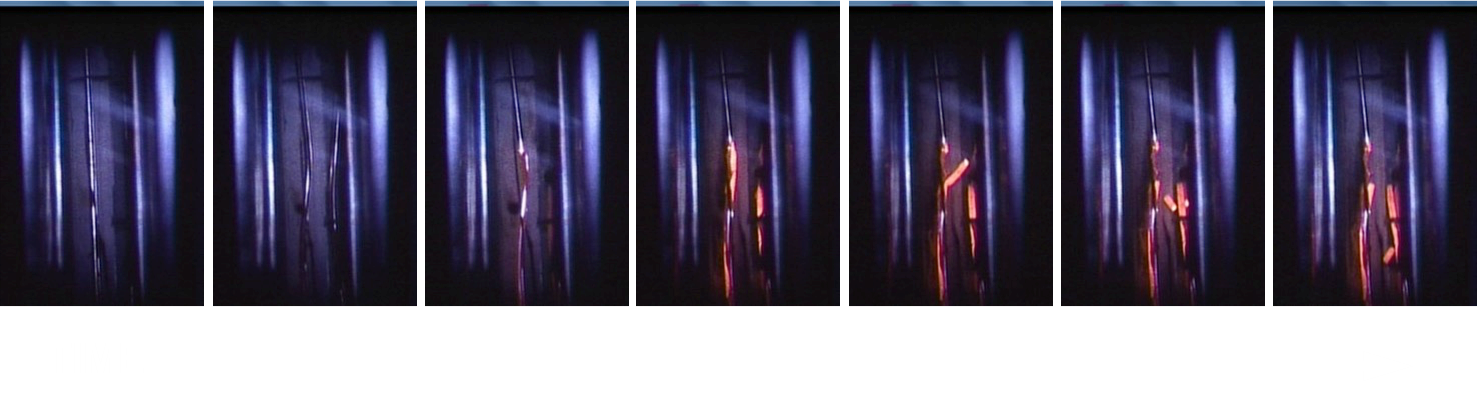
\includegraphics[height=1in]{figures/Treat_melt.png}
\end{figure}

\end{frame}
%-------------------------------------------------------------------

%------------------------------------------------------------------%
\subsection{Transient Reactor Simulation}
%------------------------------------------------------------------%

%-------------------------------------------------------------------
\begin{frame}{Modeling and experimentation are mutualistic}

\begin{figure}
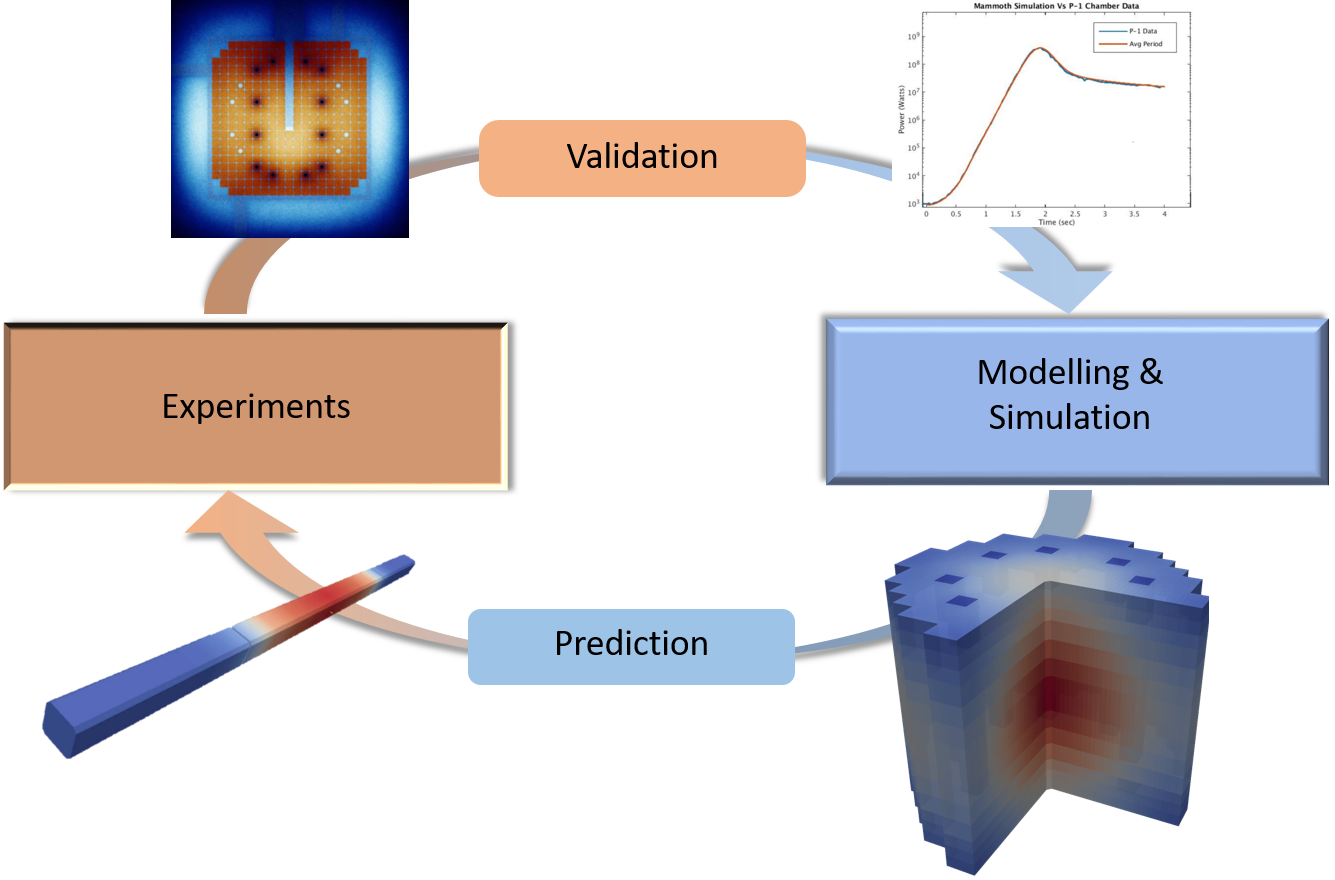
\includegraphics[width=\linewidth]{figures/relationship_chart.png}
\end{figure}

\end{frame}
%-------------------------------------------------------------------

%-------------------------------------------------------------------
\begin{frame}{Transient reactor simulation is difficult}

\begin{block}{Neutronics}
\begin{itemize}
\item Transient behavior of neutrons is typically evaluated using deterministic neutron transport to determine flux
\item Neutron transport contains 7 independent variables: time ($t$), position ($\vr$), energy ($E$), direction ($\vo$)
\item Neutron diffusion carefully eliminates direction to reduce to 5 variables
\item These equations result in a stiff system, so expensive implicit solvers are required for stability
\item Each variable needs to be discretized: FEM for space, multigroup for energy, and time will be discussed later
\end{itemize}
\end{block}

\begin{block}{Multiphysics}
\begin{itemize}
\item Reactor physics involve more than the behavior of neutrons, including: fuel temperature, thermal hydraulics, fuel structure, depletion etc.
\item All of these variables are dependent on one another, or coupled
\item Each variable have very different solution methods
\item The exponential increase in computational expense for each variable and communication between different solvers make multiphysics a daunting task
\end{itemize}
\end{block}

\end{frame}
%-------------------------------------------------------------------

%------------------------------------------------------------------%
\subsection{Improved Quasi-Static Method}
%------------------------------------------------------------------%

%-------------------------------------------------------------------
\begin{frame}{IQS mitigates neutronics expense}

\begin{block}{}
\begin{itemize}
\item IQS involves factorizing flux into space-time-energy-dependent space and time-dependent amplitude
\item Shape maintains the difficulty of flux to evaluate, but amplitude is much easier
\item The impetus of IQS is that shape is weakly dependent on time
\item Shape and amplitude can be evaluated on different time scales to maximize efficiency
\end{itemize}
\end{block}

\begin{tabular}{ccc}
\raisebox{-0.5\height}{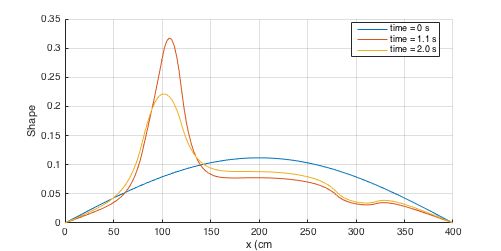
\includegraphics[height=1.15in]{figures/1D_shape.png}} &
\LARGE $\times$ &
\raisebox{-0.5\height}{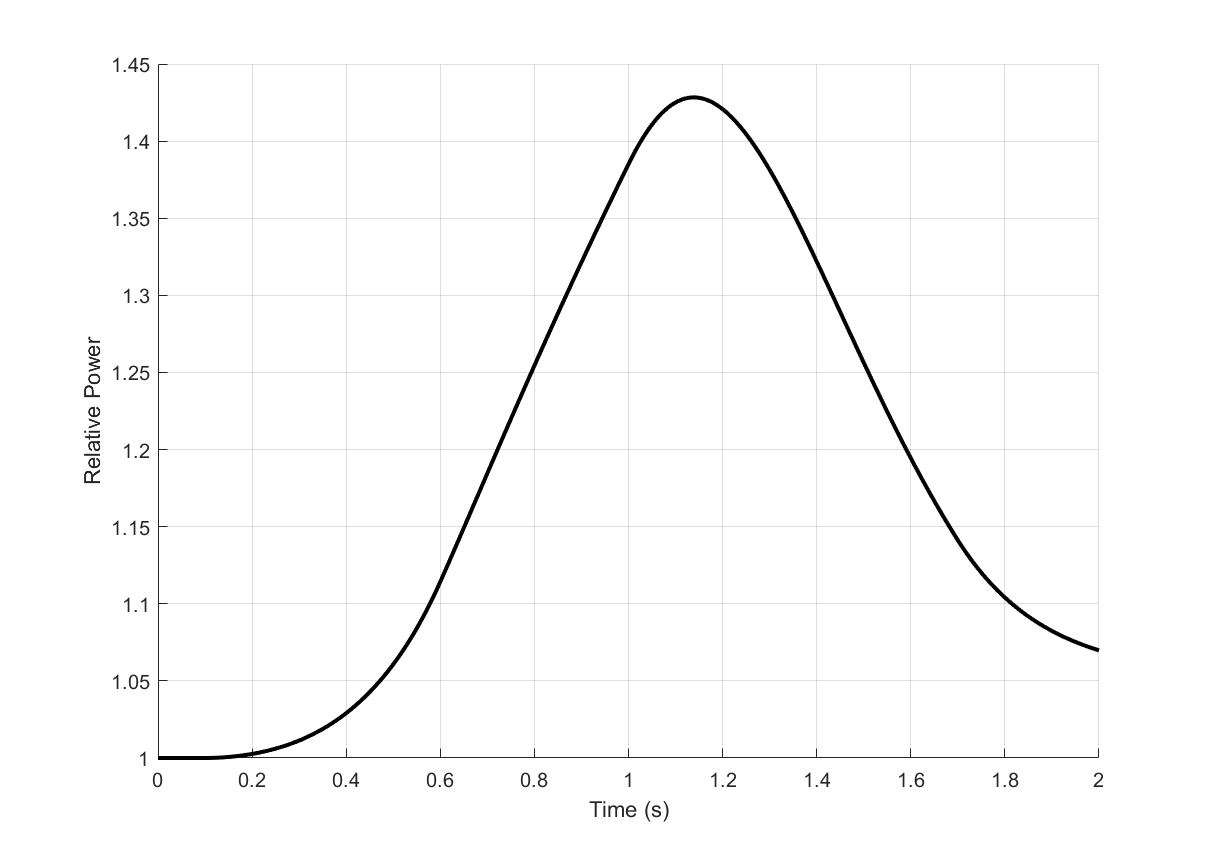
\includegraphics[height=1.15in]{figures/1D_power_base.png}} \\
Shape($\vr,E,t$) & & Amplitude($t$)
\end{tabular}

\end{frame}
%-------------------------------------------------------------------

%%%%%%%%%%%%%%%%%%%%%%%%%%%%%%%%%%%%%%%%%%%%%%%%%%%%%%%%%%%%%%%%%%%%
\section{Theory}
%%%%%%%%%%%%%%%%%%%%%%%%%%%%%%%%%%%%%%%%%%%%%%%%%%%%%%%%%%%%%%%%%%%%

%------------------------------------------------------------------%
\subsection{Neutron Diffusion}
%------------------------------------------------------------------%

%-------------------------------------------------------------------
\begin{frame}{Time-dependent Multigroup Diffusion}

\vspace{-3mm}

\begin{block}{Group Fluxes $\phi^g$ $(1 \le g \le G )$ with Precursors $C_i$ $(1 \le i \le I)$}
\begin{align*}
\frac{1}{v^g} \frac{\partial \phi^g }{\partial t} =& \frac{\chi_p^g}{\keff} \sum_{g'=1}^G (1-\beta) \nu^{g'} \Sigma_f^{g'} \phi^{g'} -  \left( -\div D^g \grad  + \Sigma_r^g \right) \phi^g  \nonumber \\
&  + \sum_{g'\neq g}^G\Sigma_s^{g'\to g} \phi^{g'}  + \sum_{i=1}^I\chi_{d,i}^g\lambda_i C_i \ , \quad 1 \le g \le G 
\end{align*}
\be
\frac{dC_i}{dt} = \frac{\beta_i}{k_{eff}}\sum_{g=1}^G\nu^{g} \Sigma_f^g \phi^{g} - \lambda_i C_i \ , \quad 1 \le i \le I 
\ee
\end{block}

\begin{block}{}
\begin{itemize}
\item Direct time discretization of these equations is termed "implicit discretization"
\item These equations are particularly stiff due to the large value of $v$
\item Implicit schemes are necessary with many time steps
\end{itemize}
\end{block}

\end{frame}
%-------------------------------------------------------------------

%------------------------------------------------------------------%
\subsection{Point Reactor Kinetics}
%------------------------------------------------------------------%

%-------------------------------------------------------------------
\begin{frame}{Point Reactor Kinetics Equation (PRKE)}

\begin{block}{Factorization}
Point reactor kinetics involve factorizing flux into space and time dependent components:
\be
\phi^g(\vr,t) = \Phi^g(\vr)\times p(t)
\ee
\end{block}

\begin{block}{PRKE}
\[
\frac{dp}{dt}=\left[\frac{\rho-\bar{\beta}}{\Lambda}\right]p+\sum_{i=1}^I\bar{\lambda}_i\xi_i
\]
\[
\frac{d\xi_i}{dt}=\frac{\bar{\beta}_i}{\Lambda}p - \bar{\lambda}_i\xi_i \quad 1 \le i \le I 
\]
\end{block}

\begin{block}{}
\begin{itemize}
\item Large assumption of time-independent spatial variance
\item Very inexpensive to evaluate after initial flux calculation
\item "Back-of-the-envelope" calculation and postprocessing
\end{itemize}
\end{block}

\end{frame}
%-------------------------------------------------------------------

%------------------------------------------------------------------%
\subsection{Improved Quasi-Static Method}
%------------------------------------------------------------------%

%-------------------------------------------------------------------
\begin{frame}{Improved Quasi-Static Method (IQS)}

\vspace{-3mm}

\begin{block}{IQS Factorization}
Decomposition of the multigroup flux into the product of a time-dependent \tcr{amplitude} ($\tcr{p}$) and a space-/time-dependent multigroup \tcb{shape} ($\tcb{\varphi^g}$):
\be
\phi^g(\vec{r},t) = \tcr{p(t)} \tcb{\varphi^g(\vec{r},t)}
\ee
\vspace{-5mm}
\begin{itemize}
\item Factorization is \textbf{not} an approximation.
\item Note that $\tcr{p(t)}$ and $\tcb{\varphi^g(\vec{r},t)}$ are not unique. 
\item Impetus is that $\tcb{\varphi^g(\vec{r},t)}$ is much slower varying than $\phi^g(\vec{r},t)$ and $\tcr{p(t)}$
\item Equations for $\tcb{\varphi^g(\vec{r},t)}$ and $\tcr{p(t)}$ need to be derived
\end{itemize}
\end{block}

\end{frame}
%-------------------------------------------------------------------

%-------------------------------------------------------------------
\begin{frame}{IQS Shape Equations}

\begin{block}{Shape Equations}
Implementing factorization and solving for $\tcb{\varphi^g}$:
\begin{align*}
\frac{1}{v^g} \frac{\partial \tcb{\varphi^g} }{\partial t} =& \frac{\chi_p^g}{\keff} \sum_{g'=1}^G (1-\beta) \nu^{g'} \Sigma_f^{g'} \tcb{\varphi^{g'}} -  \left( -\div D^g \grad  + \Sigma_r^g + \tcr{\frac{1}{v^g}}\tcr{\frac{1}{p}}\tcr{\frac{dp}{dt}}\right) \tcb{\varphi^g}  \nonumber \\
&  + \sum_{g'\neq g}^G\Sigma_s^{g'\to g} \tcb{\varphi^{g'}}  + \tcr{\frac{1}{p}}\sum_{i=1}^I\chi_{d,i}^g\lambda_i C_i \ , \quad 1 \le g \le G 
\end{align*}
\begin{equation*}
\frac{dC_i}{dt} = \tcr{p}\sum_{g=1}^G \nu_{d,i} \Sigma_f^g \tcb{\varphi^{g}} - \lambda_iC_i , \quad 1 \le i \le I
\end{equation*}
\end{block}

\begin{block}{Differences with original transport equation}
\ben
\item An additional removal term based on $\tcr{\frac{1}{v^g}\frac{1}{p}\frac{dp}{dt}} \tcb{\varphi^g}$
\item Delayed neutron source term scaled by $\tcr{\frac{1}{p}}$
\item The delayed fission source in the precursor equation scaled by \tcr{p}
\een
\end{block}

\end{frame}
%-------------------------------------------------------------------


%-------------------------------------------------------------------
\begin{frame}{Amplitude equations (PRKE)}

\begin{block}{Principle}
To obtain the \tcr{amplitude} equation, we multiply the shape equations with a weighting 
function (initial adjoint flux, $\phi^{*g}$), then integrate over domain.  
\end{block}

\begin{block}{Uniqueness of the factorization}
In order to impose uniqueness of the factorization, one requires:
\[
\tcp{K_0} = \sum_{g=1}^G\left(\phi^{*g},\frac{1}{v^g}\tcb{\varphi^g}\right)= constant
\]
\end{block}

\begin{block}{Notation}
\[
\left(\phi^{*g},f\right) = \int_D\phi^{*g}(\vec{r})f(\vec{r})dr^3
\]
\end{block}

\end{frame}
%-------------------------------------------------------------------

%-------------------------------------------------------------------
\begin{frame}{PRKE for IQS}
\vspace{-2mm}
\begin{block}{PRKE}
\[
\frac{d\tcr{p}}{dt}=\left[\frac{\rho-\bar{\beta}}{\Lambda}\right]\tcr{p}+\sum_{i=1}^I\bar{\lambda}_i\xi_i
\]
\[
\frac{d\xi_i}{dt}=\frac{\bar{\beta}_i}{\Lambda}\tcr{p} - \bar{\lambda}_i\xi_i \quad 1 \le i \le I 
\]
\end{block}
%\vspace{-3mm}
\begin{block}{PRKE Coefficients}

\small \be
\frac{\rho-\bar{\beta}}{\Lambda}=
\frac{ \sum_{g=1}^G \left(\phi^{*g},\sum_{g'=1}^G\frac{\chi_p^g}{\keff} \nu_p^{g'} \Sigma_f^{g'}\tcb{\varphi^{g'}} + \sum_{g'\neq g}^G\Sigma_s^{g'\to g} \tcb{\varphi^{g'}} -\left( -\div D^g \grad  + \Sigma_r^g \right)\tcb{\varphi^g}\right)}
{\sum_{g=1}^G \left(\phi^{*g},\frac{1}{v^g}\tcb{\varphi^g}\right)}
\ee \normalsize
%%
\be
\frac{\bar{\beta}}{\Lambda}=\sum_{i=1}^I\frac{\bar{\beta}_i}{\Lambda}=\frac{1}{\keff}
\frac{\sum_{i=1}^I\sum_{g=1}^G(\phi^{*g}, \beta_i\nu^{g} \Sigma_f^g \tcb{\varphi^{g}})}
{\sum_{g=1}^G \left(\phi^{*g},\frac{1}{v^g}\tcb{\varphi^g}\right)}
\ee
%%
\be
\bar{\lambda}_i=\frac{\sum_{g=1}^G(\phi^{*g},\chi_{d,i}^g\lambda_i C_i)}{\sum_{g=1}^G(\phi^{*g},\chi_{d,i}^gC_i)}
\ee

\end{block}

\end{frame}
%-------------------------------------------------------------------


%%%%%%%%%%%%%%%%%%%%%%%%%%%%%%%%%%%%%%%%%%%%%%%%%%%%%%%%%%%%%%%%%%%%
\section{Solution Methods}
%%%%%%%%%%%%%%%%%%%%%%%%%%%%%%%%%%%%%%%%%%%%%%%%%%%%%%%%%%%%%%%%%%%%

%------------------------------------------------------------------%
\subsection{Quasi-Static Process}
%------------------------------------------------------------------%

%-------------------------------------------------------------------
\begin{frame}{Quasi-Static Process}
% \vspace{-2mm}

\begin{block}{Time scales and IQS solution process}
Because solving for the \tcb{shape} can be expensive, especially in two or three dimensions, it is attractive to make the assumption that the \tcb{shape} is weakly time-dependent so the \tcb{shape} can be computed after a multitude of \tcr{PRKE} calculations:
\begin{figure}
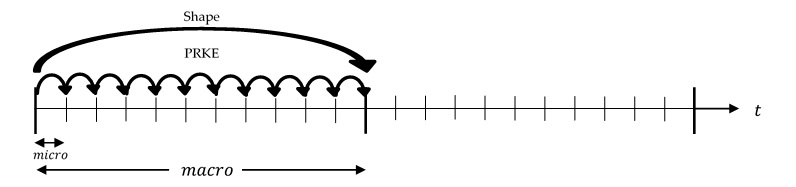
\includegraphics[width=\linewidth]{figures/IQS_visualization.jpg}
\end{figure}
\end{block}

%\begin{block}{Variable time discretization}
%\begin{itemize}
%\item To ensure stability, only implicit discretization schemes
%\item PRKE error kept constant, so either very small time steps or adaptive methods
%\item Schemes for shape include:
%\begin{itemize}
%\item Implicit Euler
%\item Crank-Nicolson
%\item Backward Difference Formulae (DDF)
%\item Singly-Diagonally-Implicit Runge-Kutta (SDIRK)
%\end{itemize}
%\end{itemize}
%\end{block}

\end{frame}
%-------------------------------------------------------------------

%-------------------------------------------------------------------
\begin{frame}{Interpolation of PRKE Parameters}

\begin{block}{Lagrange Interpolation}
\begin{itemize}
\item Parameters are evaluated at each macro step using the relevant \tcb{shape}
\item Parameters are interpolated between macro steps for PRKE
\item Most applications use linear interpolation
\item Higher order Lagrange is possible:
\be
\rho(t) = \sum_{j=0}^k \rho_{n-j+1} \prod_{m\neq j}^k \frac{t-t_{n-m+1}}{t_{n-j+1}-t_{n-m+1}}
\ee
\end{itemize}
\end{block}

\begin{figure}
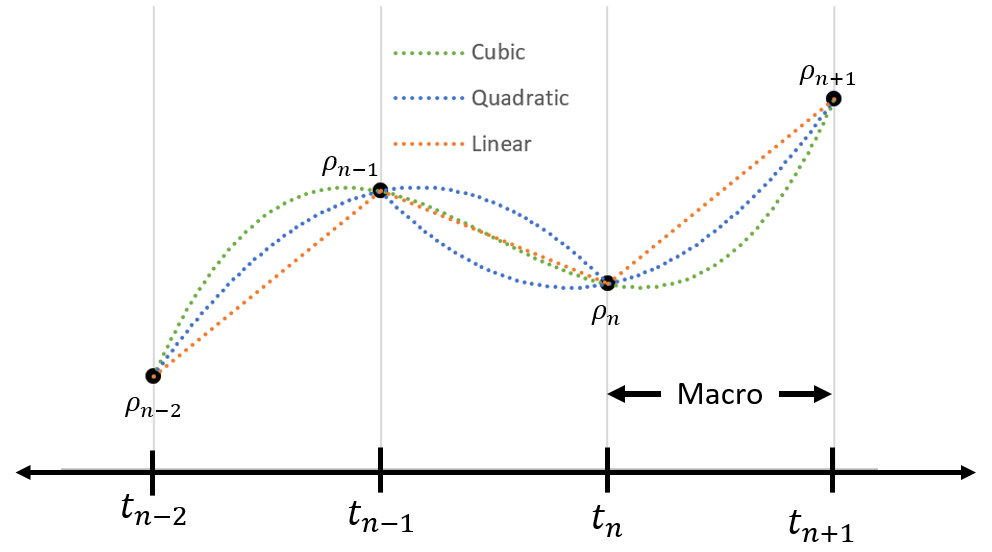
\includegraphics[height=1.5in]{figures/param_interp.png}
\end{figure}

\end{frame}
%-------------------------------------------------------------------

%------------------------------------------------------------------%
\subsection{Nonlinear Iteration}
%------------------------------------------------------------------%

%-------------------------------------------------------------------
\begin{frame}{IQS is nonlinear}

\begin{block}{Nonlinear systems need an iterative solution process}
There are two general iteration processes: 
\begin{enumerate}
\item Fixed-point (Picard): back and forth corrections between \tcr{amplitude} and \tcb{shape} with relevant convergence criteria
\item Newton: residual-Jacobian based approach on \tcb{shape}
\end{enumerate}
\end{block}

\begin{block}{Fixed-Point Process}
\begin{figure}
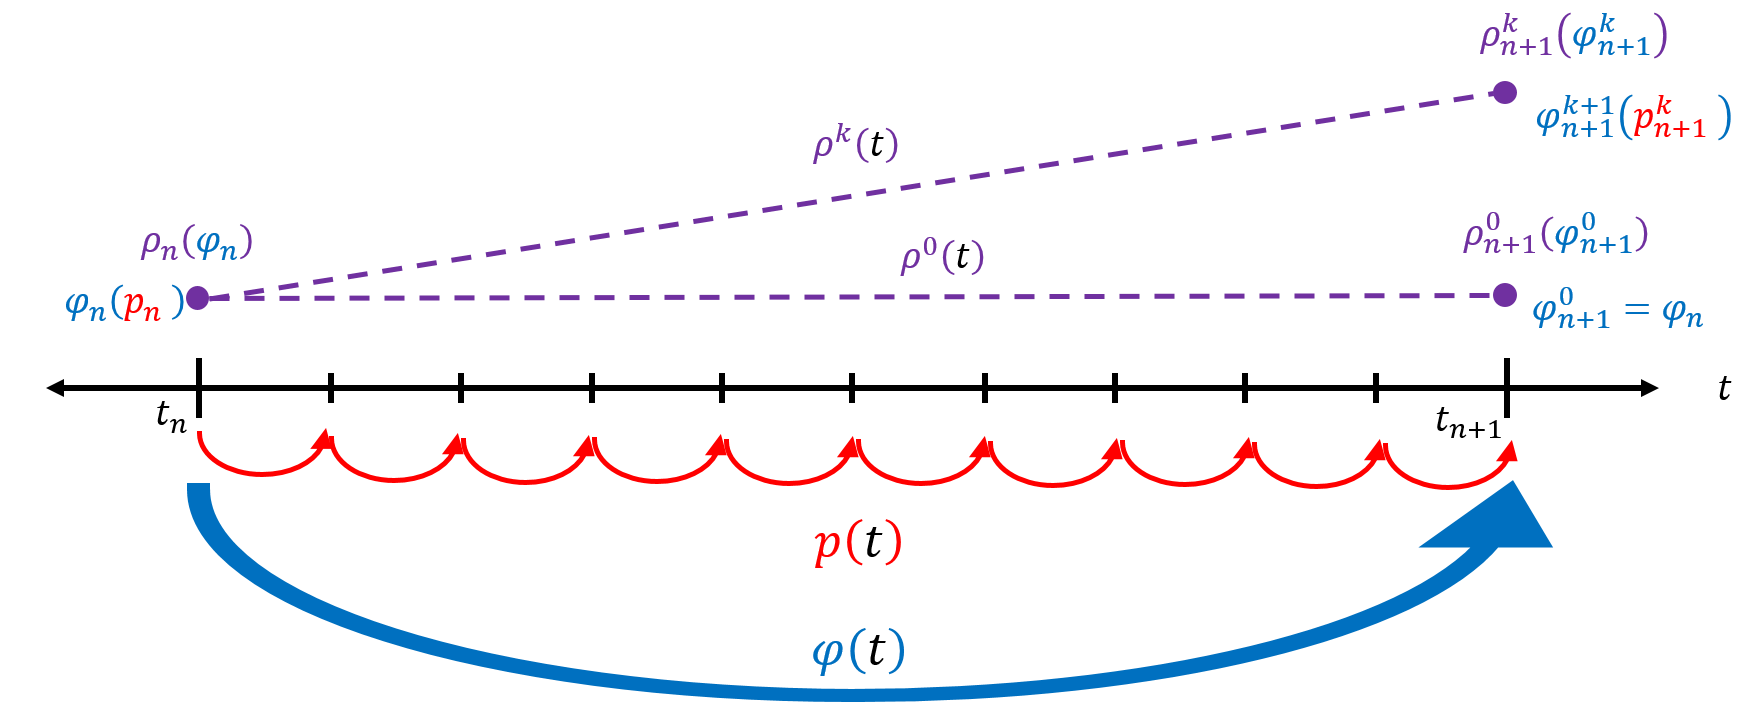
\includegraphics[width=\linewidth]{figures/iqs_iter_proc.png}
\end{figure}
\end{block}

\end{frame}
%-------------------------------------------------------------------

%-------------------------------------------------------------------
\begin{frame}{Relevant Picard convergence criteria}

\begin{block}{IQS convergence criteria}
\begin{itemize}
\item \tcb{Shape} based convergence:
\be
\frac{\text{max}\left|\tcb{\varphi{n}^{(k+1)}} - \tcb{\varphi_{n}^{(k)}}\right|}{\text{max}\left|\tcb{\varphi{n}^{(k+1)}}\right|} < \epsilon_{\varphi}
\ee 
\be
\frac{\norm{\tcb{\varphi{n}^{(k+1)}} - \tcb{\varphi_{n}^{(k)}}}}{\norm{\tcb{\varphi_{n}^{(k+1)}}}} < \epsilon_{\varphi}
\ee 

\item Reactivity based:
\be
\left(\frac{\rho}{\Lambda}\right)^{(k+1)} - \left(\frac{\rho}{\Lambda}\right)^{(k)} < \epsilon_{\rho}
\ee

\item \tcr{Amplitude} based:
\be 
\tcr{p_n^{k+1}} - \tcr{p_n^{k}} < \epsilon_p
\ee

\item Uniqueness consistency:
\be 
\frac{K_n^{(k+1)} - K_0}{K_0} < \epsilon_K
\ee
\end{itemize}
\end{block}

\end{frame}
%-------------------------------------------------------------------

%-------------------------------------------------------------------
\begin{frame}{IQS Predictor-Corrector}

\begin{block}{IQS P-C Linearizes the System}
IQS P-C linearizes the system and avoids iterations on the \tcb{shape}: 
\ben
\item Evaluate multigroup diffusion equation to get predicted flux $\phi_{n+1}^{g,\tcr{pred}}$
\item Scale predicted flux to obtain \tcb{shape}:
\[
\tcb{\varphi^{g}_{n+1}} = \phi_{n+1}^{g,\tcr{pred}} \frac{\sum_{g=1}^G\left(\phi^{*g},\frac{1}{v^g}\phi ^g_{0}\right)}{\sum_{g=1}^G \left(\phi^{*g},\frac{1}{v^g}\phi_{n+1}^{g,\tcr{pred}}\right)} = \phi_{n+1}^{g,\tcr{pred}} \frac{\tcp{K_0}}{\tcp{K_{n+1}}}
\]
\item Compute PRKE parameters at $t_{n+1}$
\item Evaluate PRKE along micro step using interpolated parameters to obtain $\tcr{p_{n+1}}$
\item Scale $\tcb{\varphi^{g}_{n+1}}$ to obtain corrected flux:
\[
\phi_{n+1}^{g,\tcr{corr}} = \tcr{p_{n+1}} \times \tcb{\varphi^{g}_{n+1}}
\]
\een

 Advantage: No IQS nonlinear iteration is necessary \\
 Disadvantage: Assumes $\sum_{g=1}^G\left(\phi^{*g},\frac{1}{v^g}\varphi^g_{n+1}\right)$ is inherently constant \\
\end{block}

\end{frame}
%-------------------------------------------------------------------

%------------------------------------------------------------------%
\subsection{Time Discretization}
%------------------------------------------------------------------%

%-------------------------------------------------------------------
\begin{frame}{Time Discretization}
\vspace{-3mm}

\begin{block}{Time Discretizations}
\begin{itemize}
\item Implicit Euler - 1st Order
\item Crank-Nicolson - 2nd Order
\item Backward Difference Formulae (BDF) - 1st, 2nd, 3rd, 4th Order
\item Singly-Diagonally-Implicit Runge-Kutta (SDIRK) - 3rd Order (SDIRK33)
\end{itemize}
\end{block}

\begin{block}{Time Step Adaptation}
\begin{itemize}
\item Determining appropriate time step is difficult without prior knowledge of the solution
\item Some areas of the transient may require smaller time steps for constant accuracy
\item Time adaptation predicts the local truncation error and computes a time step appropriate for a given tolerance
\item Examples:
\begin{itemize}
\item Step doubling
\item Embedded Runge-Kutta
\end{itemize}
\end{itemize}
\end{block}

\end{frame}
%-------------------------------------------------------------------

%-------------------------------------------------------------------
\begin{frame}{Step doubling time adaption was chosen for testing}

\begin{block}{Step Doubling Solution Process}

\begin{figure}[htpb!]
\centering
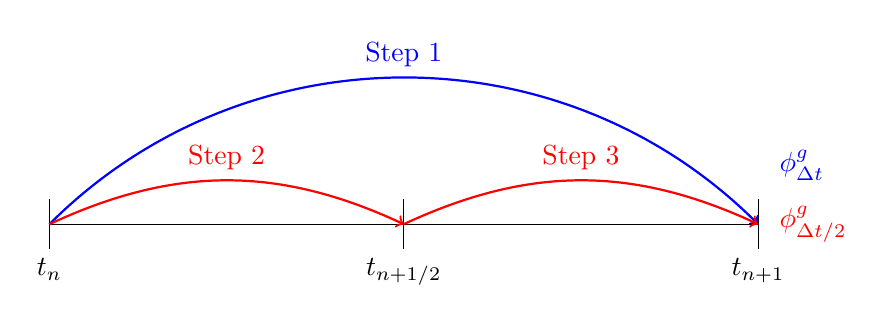
\begin{tikzpicture}[scale=1.5]
\draw[] (0,2) -- (6,2) ;
\foreach \x in  {0,3,6}
\draw[shift={(\x,2)},color=black] (0pt,6pt) -- (0pt,-6pt);
\draw[shift={(0,2)},color=black] (0pt,0pt) -- (0pt,-6pt) node[below] {$t_n$};
\draw[shift={(3,2)},color=black] (0pt,0pt) -- (0pt,-6pt) node[below] {$t_{n+1/2}$};
\draw[shift={(6,2)},color=black] (0pt,0pt) -- (0pt,-6pt) node[below] {$t_{n+1}$};
\draw (0,2) edge[out=45,in=135,->,thick,blue] node[above,sloped] {\tcb{Step 1}} (6,2);
\draw (0,2) edge[out=25,in=155,->,thick,red] node[above,sloped] {\tcr{Step 2}} (3,2);
\draw (3,2) edge[out=25,in=155,->,thick,red] node[above,sloped] {\tcr{Step 3}} (6,2);
\node[anchor=west](shape) at (6.1,2.5) {$\tcb{\phi_{\Delta t}^g}$};
\node[anchor=west](shape) at (6.1,2) {$\tcr{\phi_{\Delta t/2}^g}$};

\end{tikzpicture}
\end{figure}
\be
e_n =\frac{\norm{\sum_{g=1}^G \left(\tcr{\phi^g_{\Delta t/2}} - \tcb{\phi^g_{\Delta t}} \right)}}{\max\left(\norm{\sum_{g=1}^G\tcr{\phi^g_{\Delta t/2}}},\norm{\sum_{g=1}^G\tcb{\phi^g_{\Delta t}}}\right)} 
\qq  \qq 
\Delta t_{new} = S_f \Delta t \left[\frac{e_{tol}}{e_n}\right]^{1/(p+1)}   
\ee

\end{block}

\end{frame}
%-------------------------------------------------------------------

%-------------------------------------------------------------------
\begin{frame}{Step Doubling Solution Process}

\begin{block}{Programming Visualization}

\begin{figure}[!htpb]
\centering
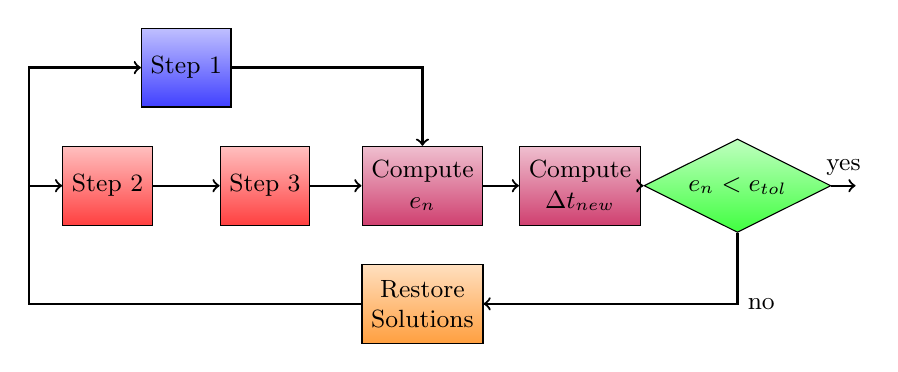
\begin{tikzpicture}[every node/.style = {font=\small},scale=0.5]

\node[blueblock](p1) at (-6,3) {Step 1} ;
\node[redblock](p2) at (-8,0) {Step 2} ;
\node[redblock](p3) at (-4,0) {Step 3} ;
\node[purpleblock](p4) at (0,0) {Compute \\ $e_n$};
\node[purpleblock](p5) at (4,0) {Compute  \\ $\Delta t_{new}$};
\node[greendiamond](p6) at (8,0) {$e_n < e_{tol}$};
\node[orangeblock](p7) at (0,-3) {Restore \\ Solutions};

\draw[->,thick](p1.east) -| (p4.north);
\draw[->,thick](p2.east) -- (p3.west);
\draw[->,thick](p3.east) -- (p4.west);
\draw[->,thick](p4.east) -- (p5.west);
\draw[->,thick](p5.east) -- (p6.west);
\draw[->,thick](p6.south) |- node[right] {no} (p7.east);
\draw[->,thick](p6.east) -- node[above] {yes} (11,0);
\draw[->,thick](p7.west) -| (-10,0) -- (p2.west);
\draw[->,thick](p7.west) -| (-10,0) |- (p1.west);

\end{tikzpicture}
\end{figure}
Each Step undergoes:
\bi
\item Shape evaluation
\item PRKE evaluations
\item Multiphysics evaluations
\item Iterations for convergence of amplitude, shape, and multiphysics
\ei

\end{block}

\end{frame}
%-------------------------------------------------------------------

%------------------------------------------------------------------%
\subsection{Delayed Neutron Precursors}
%------------------------------------------------------------------%

%-------------------------------------------------------------------
\begin{frame}{Treatment of delayed neutron precursors}
\vspace{-3mm}
\begin{block}{Delayed neutron precursor equation is an ODE}
\begin{equation*}
\frac{dC_i}{dt} = \tcr{p}\sum_{g=1}^G \beta_i\nu \Sigma_f^g \tcb{\varphi^{g}} - \lambda_iC_i , \quad 1 \le i \le I
\end{equation*}
\end{block}

\begin{block}{Time Integration of Precursors}
\begin{itemize}
\item Trapezoid Rule:
\be
C^{n+1}_i = \frac{1-0.5\Delta t\lambda_i}{1+0.5\Delta t\lambda_i}C^n_i + \frac{0.5\Delta t \beta_i}{1+0.5\Delta t\lambda_i}\sum_{g=1}^G\left[(\nu\Sigma_f^g\tcb{\varphi^g})^n \tcr{p^n} +  (\nu\Sigma_f^g\tcb{\varphi^g})^{n+1} \tcr{p^{n+1}}\right]
\ee
\item Analytical Integration:
\be 
C^{n+1}_i = C^n_i e^{-\lambda_i \Delta t} + \sum_{g=1}^G\left(\hat{a}_{2,i} (\nu\Sigma_f^g\tcb{\varphi^g})^{n+1}+\hat{a}_{1,i} (\nu\Sigma_f^g\tcb{\varphi^g})^n\right)\beta_i
\ee
\vspace{-4mm}
\begin{align*}
&\hat{a}_{1,i}= \int_{t_n}^{t_{n+1}}\frac{t_{n+1}-t'}{\Delta t}\tcr{p(t')}e^{-\lambda_i(t_{n+1}-t')}dt' \\
&\hat{a}_{2,i} = \int_{t_n}^{t_{n+1}}\frac{t'-t_n}{\Delta t}\tcr{p(t')}e^{-\lambda_i(t_{n+1}-t')}dt'
\end{align*}
\end{itemize}
\end{block}

\end{frame}
%-------------------------------------------------------------------

%------------------------------------------------------------------%
\subsection{Temperature Feedback}
%------------------------------------------------------------------%

%-------------------------------------------------------------------
\begin{frame}{Multiphysics: Adiabatic heat-up with absorption cross-section feedback}

\begin{block}{Implemented Form}
\be
\rho c_p \frac{\partial T(\vec{r},t)}{\partial t} = \kappa_f \sum^G_{g=1}\Sigma_f^g \tcb{\varphi^g(\vec{r},t)}\tcr{p(t)}
\ee
\be
\Sigma_a^{thermal}(\vec{r},t) = \Sigma_a^{thermal}(\vec{r},0)\left[1+\gamma\left(\sqrt{T}-\sqrt{T_0}\right)\right]
\ee
\end{block}

\begin{block}{Analytical temperature integration with IQS}
\be
T^{n+1} = T^n + \frac{\kappa_f}{\rho c_p} \sum_{g=1}^G\left(a_2(\Sigma_f^g\tcb{\varphi^g})^{n+1} + a_1(\Sigma_f^g\tcb{\varphi^g})^n\right)
\label{eq:temp_an}
\ee
\be
a_1 = \int_{t_n}^{t_{n+1}}\left(\frac{t_{n+1}-t'}{\Delta t}\right)\tcr{p(t')}dt'
\label{eq:a1}
\ee
\be
a_2 = \int_{t_n}^{t_{n+1}}\left(\frac{t'-t_n}{\Delta t}\right)\tcr{p(t')}dt'
\label{eq:a2}
\ee
\end{block}

\end{frame}
%-------------------------------------------------------------------

%-------------------------------------------------------------------
\begin{frame}{Intermediate time scale for temperature}



\begin{figure}
\resizebox{\linewidth}{!}{
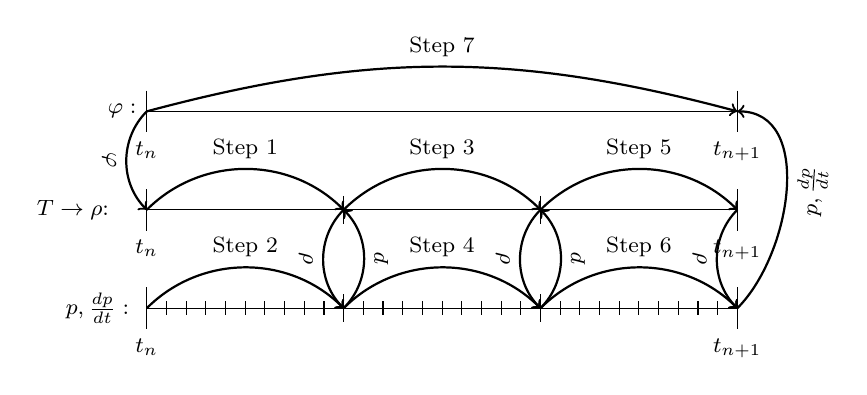
\begin{tikzpicture}[scale=1.25]
\tikzset{font={\footnotesize}}
%Shape
\draw[] (0,2) -- (6,2) ;
\foreach \x in  {0,6}
\draw[shift={(\x,2)},color=black] (0pt,6pt) -- (0pt,-6pt);
\draw[shift={(0,2)},color=black] (0pt,0pt) -- (0pt,-6pt) node[below] {$t_n$};
\draw[shift={(6,2)},color=black] (0pt,0pt) -- (0pt,-6pt) node[below] {$t_{n+1}$};
\node(shape) at (-.25,2) {$\varphi:$};

%Temp/Params
\draw[] (0,1) -- (6,1) ;
\foreach \x in  {0,6}
\draw[shift={(\x,1)},color=black] (0pt,6pt) -- (0pt,-6pt);
\foreach \x in  {2,4}
\draw[shift={(\x,1)},color=black] (0pt,4pt) -- (0pt,-4pt);
\draw[shift={(0,1)},color=black] (0pt,0pt) -- (0pt,-6pt) node[below] {$t_n$};
\draw[shift={(6,1)},color=black] (0pt,0pt) -- (0pt,-6pt) node[below] {$t_{n+1}$};
\node(temp) at (-.75,1) {$T \rightarrow \rho$:};

% PRKE
\draw[] (0,0) -- (6,0) ;
\foreach \x in  {0,6}
\draw[shift={(\x,0)},color=black] (0pt,6pt) -- (0pt,-6pt);
\foreach \x in  {0,2,4,6}
\draw[shift={(\x,0)},color=black] (0pt,4pt) -- (0pt,-4pt);
\foreach \x in  {0,0.2,0.4,0.6,0.8,1,1.2,1.4,1.6,1.8,2,2.2,2.4,2.6,2.8,3,3.2,3.4,3.6,3.8,4,4.2,4.4,4.6,4.8,5,5.2,5.4,5.6,5.8,6}
\draw[shift={(\x,0)},color=black] (0pt,2pt) -- (0pt,-2pt);
\draw[shift={(0,0)},color=black] (0pt,0pt) -- (0pt,-6pt) node[below] {$t_n$};
\draw[shift={(6,0)},color=black] (0pt,0pt) -- (0pt,-6pt) node[below] {$t_{n+1}$};
\node(prke) at (-.5,0) {$p, \frac{dp}{dt}:$};

\draw (0,0) edge[out=45,in=135,->,thick] node[above,sloped] {Step 2} (2,0);
\draw (2,0) edge[out=45,in=135,->,thick] node[above,sloped] {Step 4} (4,0);
\draw (4,0) edge[out=45,in=135,->,thick] node[above,sloped] {Step 6} (6,0);
\draw (0,1) edge[out=45,in=135,->,thick] node[above,sloped] {Step 1} (2,1);
\draw (2,1) edge[out=45,in=135,->,thick] node[above,sloped] {Step 3} (4,1);
\draw (4,1) edge[out=45,in=135,->,thick] node[above,sloped] {Step 5} (6,1);
\draw (0,2) edge[out=15,in=165,->,thick] node[above,sloped] {Step 7} (6,2);

\draw (0,2) edge[out=-135,in=135,->,thick] node[below,sloped] {$\varphi$} (0,1);
\draw (2,1) edge[out=-135,in=135,->,thick] node[below,sloped] {$\rho$} (2,0);
\draw (2,0) edge[out=45,in=-45,->,thick] node[below,sloped] {$p$} (2,1);
\draw (4,1) edge[out=-135,in=135,->,thick] node[below,sloped] {$\rho$} (4,0);
\draw (4,0) edge[out=45,in=-45,->,thick] node[below,sloped] {$p$} (4,1);
\draw (6,1) edge[out=-135,in=135,->,thick] node[below,sloped] {$\rho$} (6,0);
\draw (6,0) edge[out=45,in=0,->,thick] node[below,sloped] {$p, \frac{dp}{dt}$} (6,2);

\end{tikzpicture}
}
\end{figure}

\end{frame}
%-------------------------------------------------------------------

%-------------------------------------------------------------------
\begin{frame}{Time scale programming logic}

\begin{figure}
\centering
\resizebox{!}{3in}{
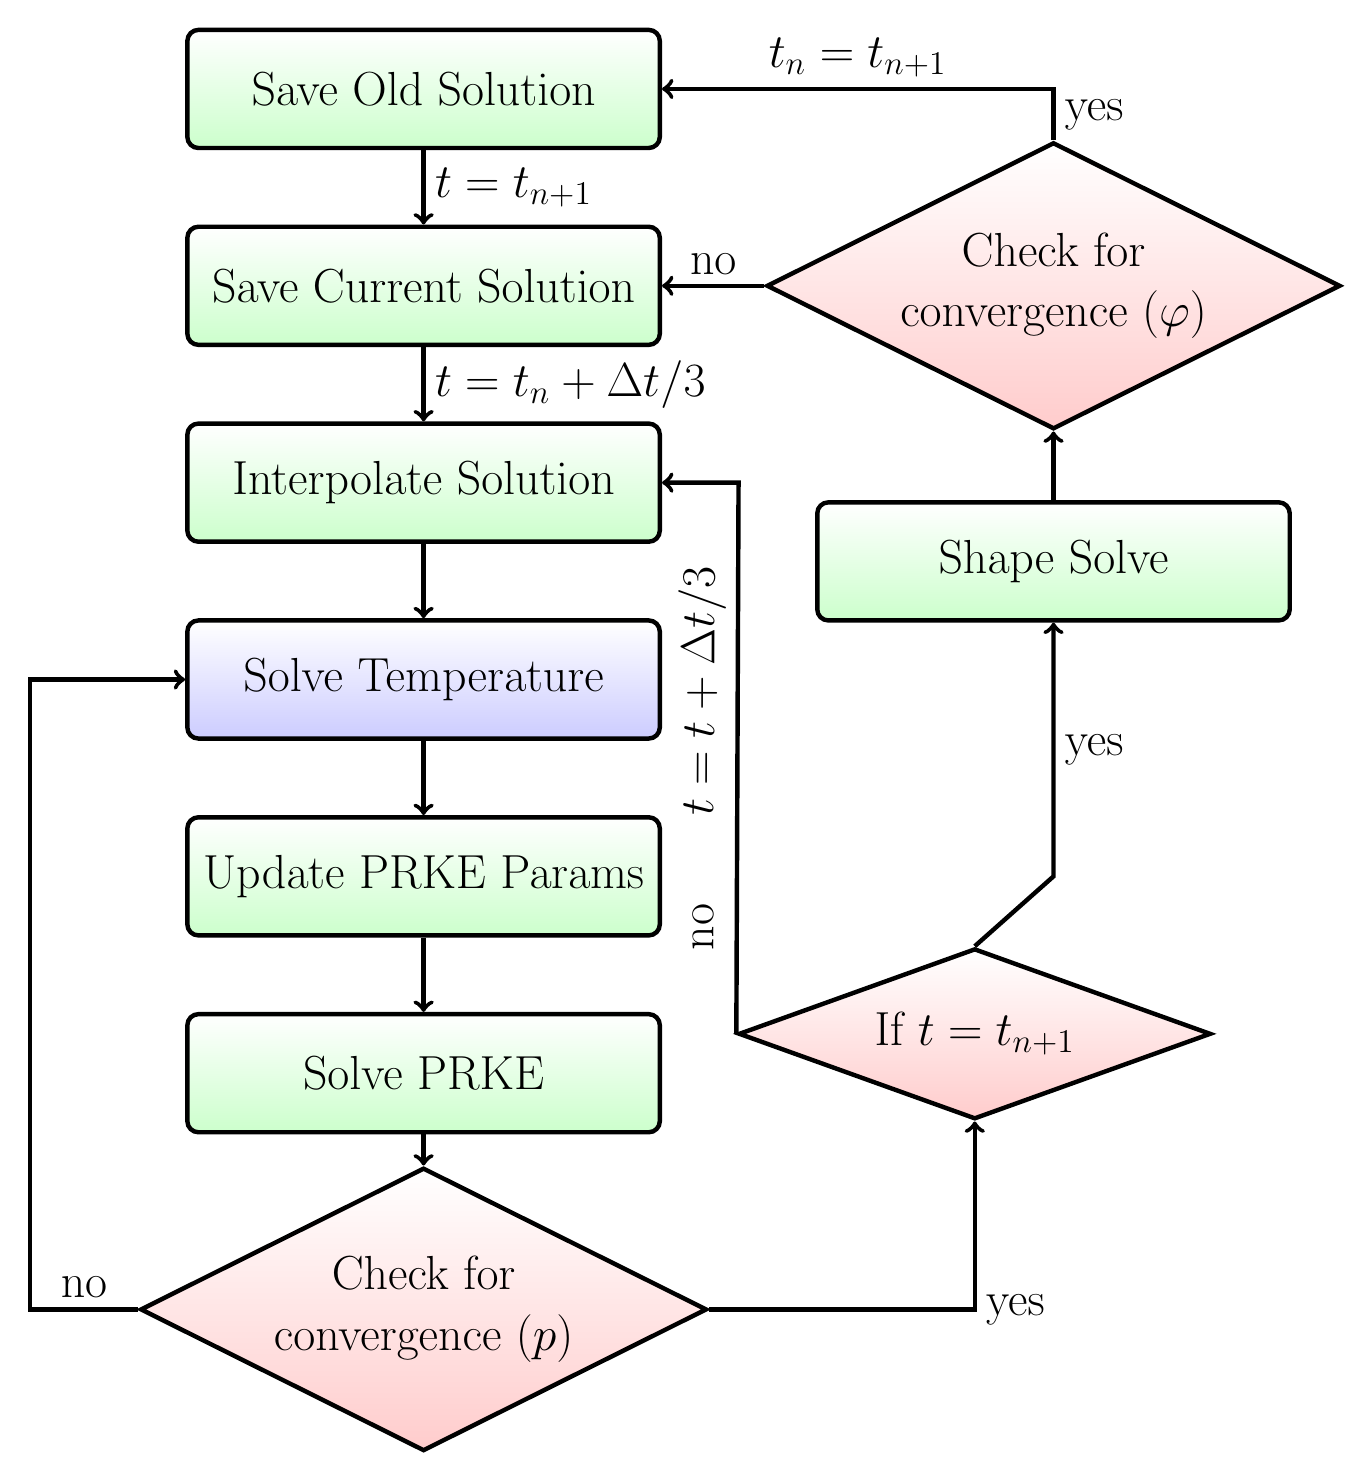
\begin{tikzpicture}[every node/.style = {font=\LARGE}]

\node[greenblock](p1) at (0,0) {Save Old Solution};
\node[greenblock](p2) at (0,-2.5) {Save Current Solution};
\node[greenblock](p3) at (0,-5) {Interpolate Solution};
\node[blueblock2](p4) at (0,-7.5) {Solve Temperature};
\node[greenblock] (p5) at (0,-10) {Update PRKE Params};
\node[greenblock] (p6) at (0,-12.5) {Solve PRKE};
\node[reddiamond] (check1) at (0,-15.5) {Check for \\ convergence ($p$)};
\node[reddiamond] (check2) at (7,-12) {If $t=t_{n+1}$};
\node[greenblock] (p7) at (8,-6) {Shape Solve};
\node[reddiamond] (check3) at (8,-2.5) {Check for \\ convergence ($\varphi$)};
%\node [above =0.1mm of p1] {\large{IQS Solve:}};
%\node [above =0.1mm of p5] {\large{Multi-physics:}};

%\tikzback{p1}{p1}{p4}{p4}{bk1}
%\tikzback{p5}{p5}{p5}{p5}{bk2}

\draw[->,ultra thick](p1.south) -- node[right] {$t=t_{n+1}$}(p2.north);
\draw[->,ultra thick](p2.south) -- node[right] {$t=t_{n}+\Delta t/3$}(p3.north);
\draw[->,ultra thick](p3.south) -- (p4.north);
\draw [->,ultra thick] (p4.south)-- (p5.north);
\draw[->,ultra thick](p5.south) -- (p6.north);
\draw[->,ultra thick](p6.south) -- (check1.north);
\draw[->,ultra thick](check1.west) -- node[above,sloped] {\LARGE{no}} (-5,-15.5) |-  (p4.west);
\draw[->,ultra thick](check1.east) -| node[right] {\LARGE{yes}} (check2.south);
\draw[->,ultra thick](check2.west) -- node[above,sloped] {\LARGE{no}\LARGE \qq $t=t+\Delta t/3$} (4,-5) -- (p3.east);
\draw[->,ultra thick](check2.north) --  (8,-10) -- node[right] {\LARGE{yes}} (p7.south);
\draw[->,ultra thick](p7.north) -- (check3.south);
\draw[->,ultra thick](check3.west) -- node[above] {no} (p2.east);
\draw[->,ultra thick](check3.north) -- node[right] {yes} (8,0) -- node[above] {$t_n=t_{n+1}$} (p1.east);

\end{tikzpicture}
}
\end{figure}

\end{frame}
%-------------------------------------------------------------------

%-------------------------------------------------------------------
\begin{frame}{Time Scale Analysis}

\begin{block}{Dynamical Time Scale}
\begin{itemize}
\item The time variance of each physics ($\theta$) can be quantified by defining a dynamical time scale ($\tau$):
\be
\tau = \frac{1}{\left|\frac{1}{\theta}\frac{d\theta}{dt}\right|}
\ee
\item Finite difference approximation for $d\theta/dt$ and average for $1/\theta$
\item Only temporal behavior is of interest, so the $L^2$ norm will be taken of each quantity, resulting in:
\be
\tilde{\tau}_{n+1} = \frac{\norm{\theta_{n+1} + \theta_{n}}}{2}\frac{\Delta t}{\norm{\theta_{n+1} - \theta_{n}}}
\ee
\item According to the a priori hypothesis, $\tau$ is large for \tcb{shape}, somewhat smaller for temperature, and much smaller for \tcr{amplitude} and flux
\end{itemize}
\end{block}

\end{frame}
%-------------------------------------------------------------------

\addtocontents{toc}{\newpage}
%%%%%%%%%%%%%%%%%%%%%%%%%%%%%%%%%%%%%%%%%%%%%%%%%%%%%%%%%%%%%%%%%%%%
\section{Implementation}
%%%%%%%%%%%%%%%%%%%%%%%%%%%%%%%%%%%%%%%%%%%%%%%%%%%%%%%%%%%%%%%%%%%%

%------------------------------------------------------------------%
\subsection{MATLAB Prototype}
%------------------------------------------------------------------%

%-------------------------------------------------------------------
\begin{frame}{MATLAB Kinetics Prototype Code}

\begin{block}{Overview}
\begin{itemize}
\item One-dimensional, single-group, time-dependent neutron diffusion with precursors
\item Heterogenous medium using block-like regions
\item Step and ramp perturbations in parameters
\item Manufactured solutions using symbolic capability
\item FEM meshing with any order shape functions
\end{itemize}
\end{block}

\begin{block}{Solution Methods}
\begin{multicols}{2}
\begin{enumerate}
\item Implicit Discretization
\begin{itemize}
\item Precursor variable coupling
\item Theta precursor elimination
\item Analytical precursor elimination
\end{itemize}
\item IQS
\begin{itemize}
\item Precursor variable coupling
\item Theta precursor elimination
\item Analytical precursor elimination
\end{itemize}
\item IQS P-C
\begin{itemize}
\item Theta precursor elimination
\item Analytical precursor elimination
\end{itemize}
\end{enumerate}
\end{multicols}
\end{block}

\end{frame}
%-------------------------------------------------------------------

%------------------------------------------------------------------%
\subsection{MOOSE/Rattlesnake}
%------------------------------------------------------------------%

%-------------------------------------------------------------------
\begin{frame}{Reactor Simulation in MOOSE}

\begin{figure}
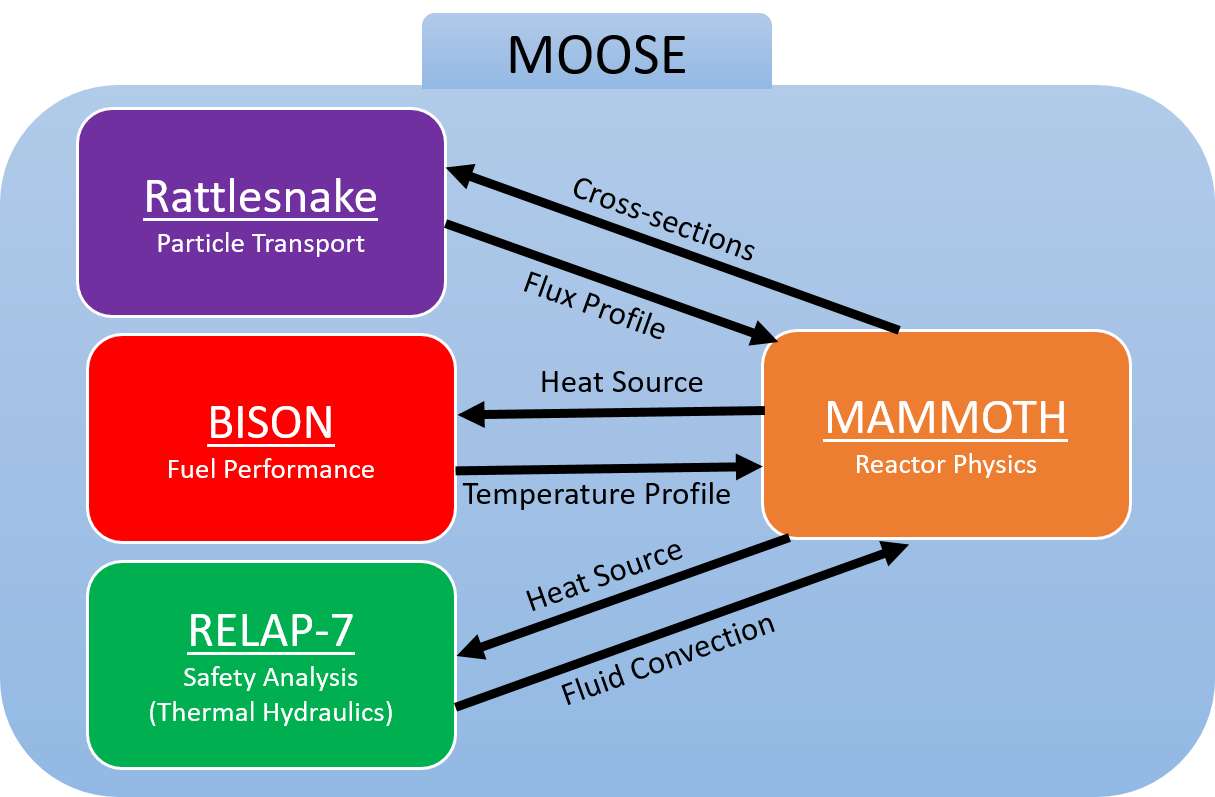
\includegraphics[width=\linewidth]{figures/mammoth.png}
\end{figure}

\end{frame}
%-------------------------------------------------------------------

%%%%%%%%%%%%%%%%%%%%%%%%%%%%%%%%%%%%%%%%%%%%%%%%%%%%%%%%%%%%%%%%%%%%
\section{Results}
%%%%%%%%%%%%%%%%%%%%%%%%%%%%%%%%%%%%%%%%%%%%%%%%%%%%%%%%%%%%%%%%%%%%

%-------------------------------------------------------------------
\begin{frame}{Results}

\begin{multicols}{2}
\tableofcontents[currentsection]
\end{multicols}

\end{frame}
%-------------------------------------------------------------------

%------------------------------------------------------------------%
\subsection{One-Dimensional Slab}
%------------------------------------------------------------------%

%-------------------------------------------------------------------
\begin{frame}{One Dimensional Example}

\begin{block}{Geometry}
\begin{figure}
\begin{center}
\resizebox{\linewidth}{!}{
\begin{tabular}{| l | l | l | l | l | l | l | l | l | l | l | l | l | l | l | l | l | l | l | l |}
\hline \hline \hline
  &   &   &   &   &   &    &    &   &   &   &   &   &   &   &   &   &   &   &   \\
1 & 1 & 1 & 1 & 2 & 3 & 1 & 1 & 1 & 1 & 1 & 1 & 1 & 1 & 4 & 4 & 1 & 1 & 1 & 1 \\
  &   &   &   &   &   &    &    &   &   &   &   &   &   &   &   &   &   &   &   \\
\hline \hline \hline
\end{tabular}}
\end{center}
\end{figure}
\begin{itemize}
\item Region 2: Ramp $\Sigma_a$ decrease (rod removal)
\item Region 3: Ramp $\Sigma_a$ decrease then increase (rod removal then insertion)
\item Region 4: Ramp $\Sigma_a$ increase (rod insertion)
\end{itemize}
\end{block}

\begin{block}{Region Perturbations}
\centering
\begin{tabular}{llllllll}
\hline
Region & Material Property & 0.0 s & 0.1 s & 0.6 s & 1.0 s & 1.7 s \\
\hline
2 & $\Sigma_{a} (cm^{-1})$ & 1.1 & 1.1 & 1.095 & 1.095 & 1.095 \\
3 & $\Sigma_{a} (cm^{-1})$ & 1.1 & 1.1 & 1.09 & 1.09 & 1.1 \\
4 & $\Sigma_{a} (cm^{-1})$ & 1.1 & 1.1 & 1.105 & 1.105 & 1.105 \\
\hline
\end{tabular}
\end{block}

\end{frame}
%-------------------------------------------------------------------

%-------------------------------------------------------------------
\begin{frame}{Baseline Results}

\begin{columns}
\column{\dimexpr\paperwidth-10pt}
\begin{figure}
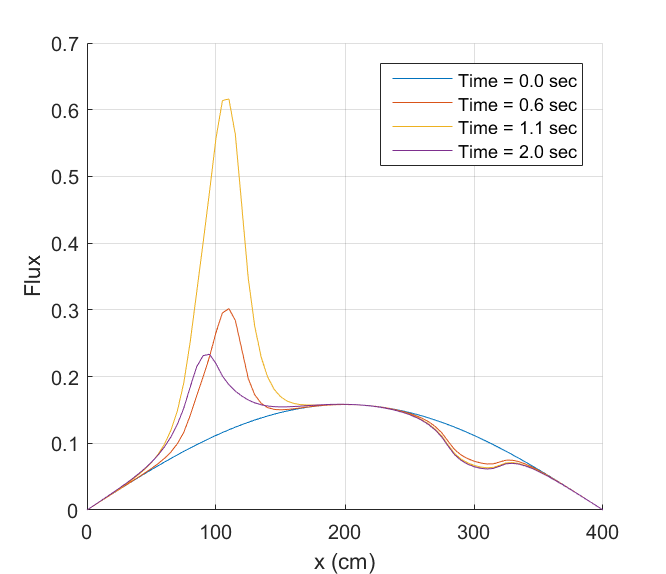
\includegraphics[width=0.45\linewidth]{figures/1D_flux.png}
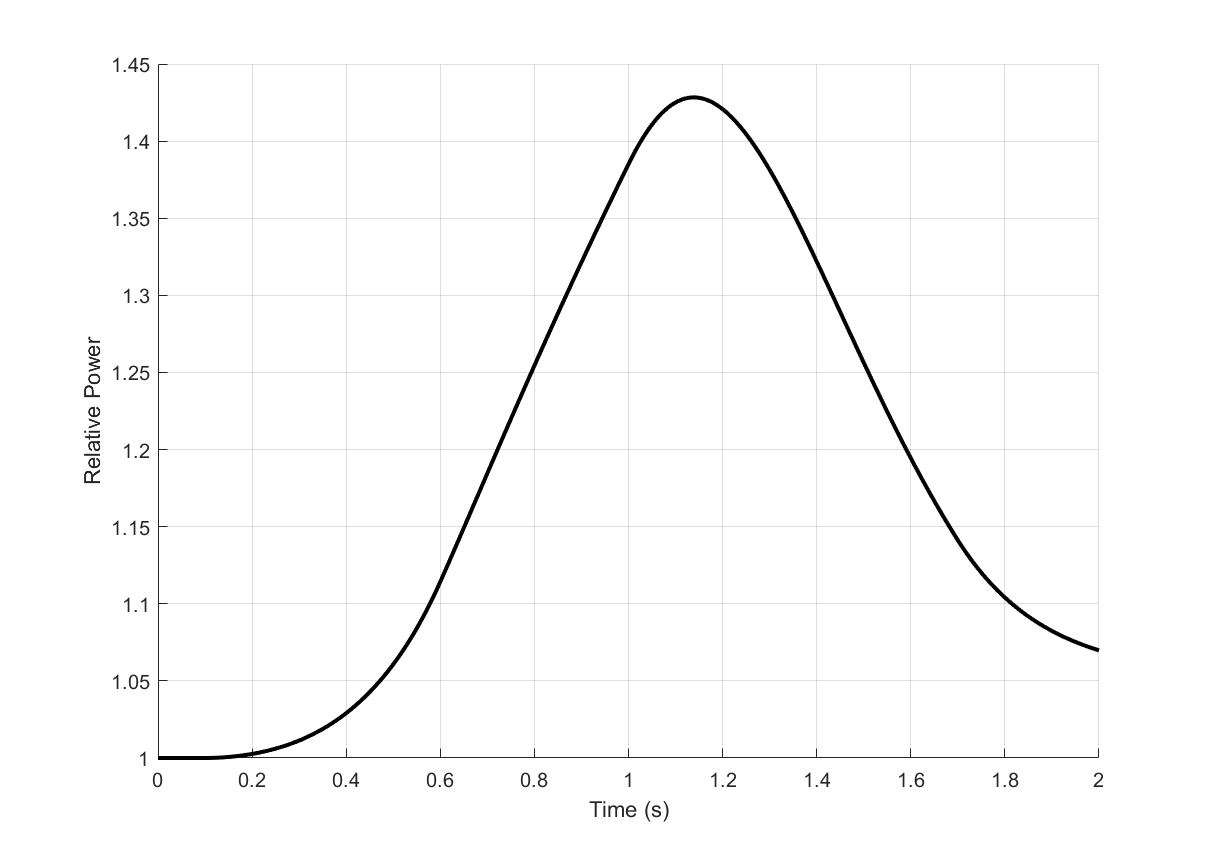
\includegraphics[width=0.55\linewidth]{figures/1D_power_base.png}
\end{figure}
\end{columns}

\end{frame}
%-------------------------------------------------------------------

%-------------------------------------------------------------------
\begin{frame}{IQS Results}

\begin{columns}
\column{\dimexpr\paperwidth-10pt}
\begin{figure}
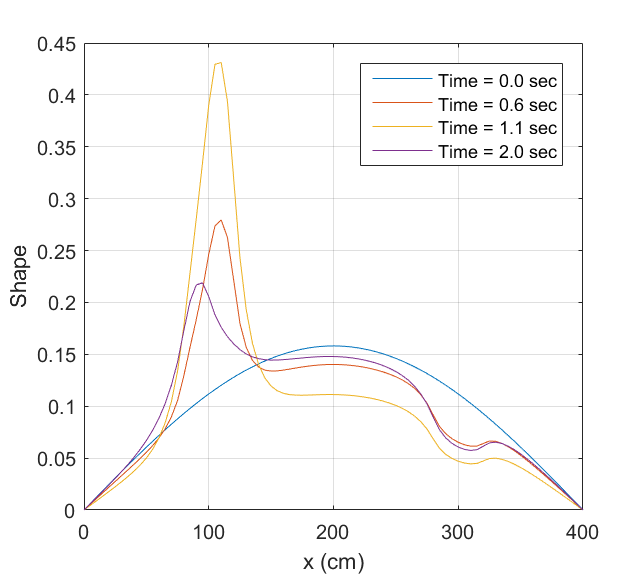
\includegraphics[width=0.45\linewidth]{figures/1D_shape2.png}
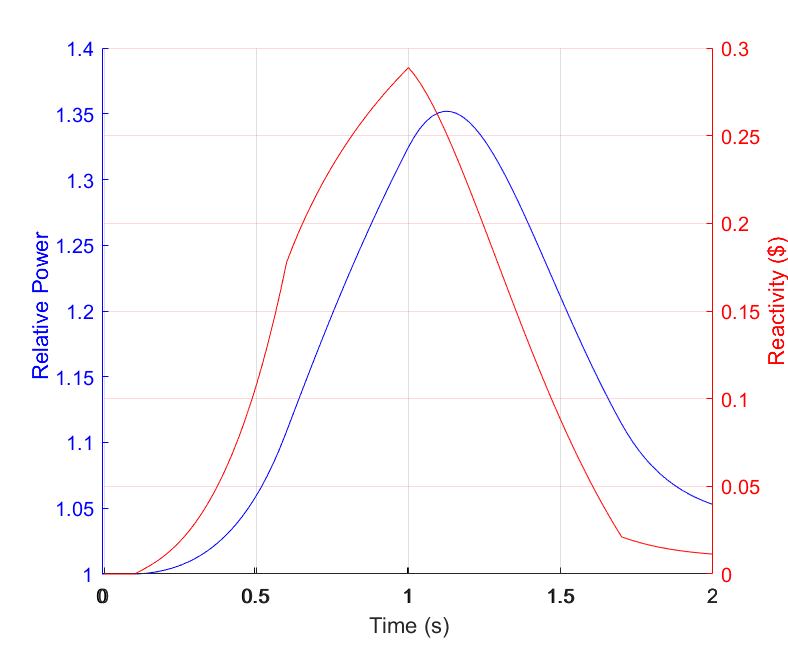
\includegraphics[width=0.55\linewidth]{figures/1D_iqs_power.png}
\end{figure}
\end{columns}

\end{frame}
%-------------------------------------------------------------------

%-------------------------------------------------------------------
\begin{frame}{Convergence criteria convergence behavior}

\begin{figure}
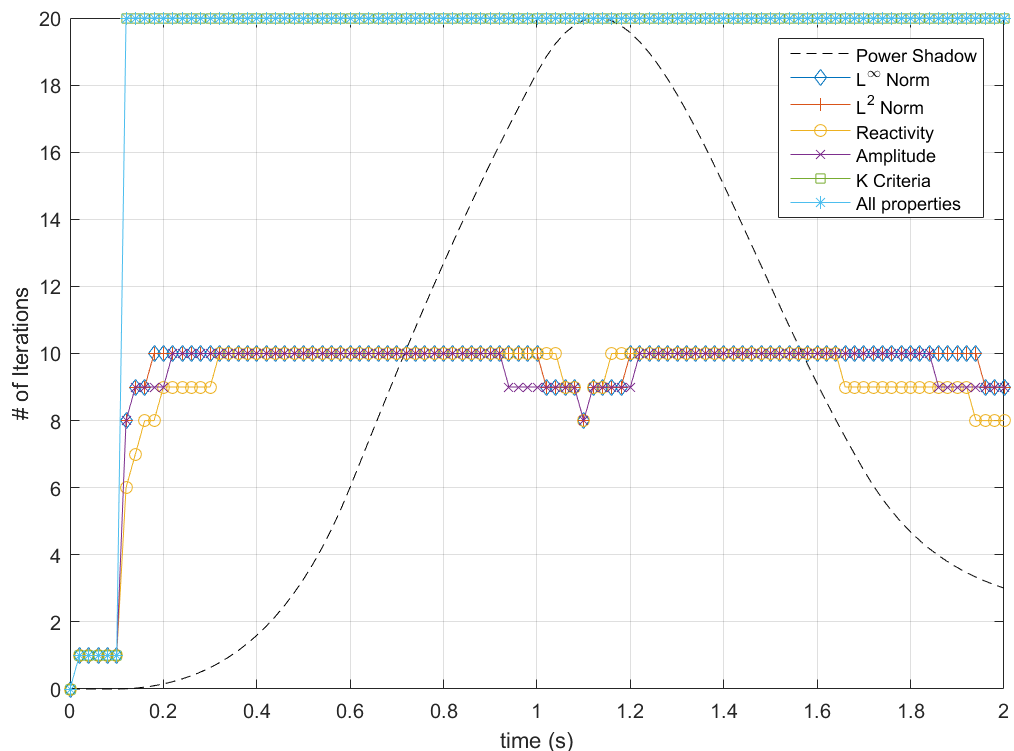
\includegraphics[width=\linewidth,height=3in,keepaspectratio]{figures/iter_renorm.png}
\end{figure}

\end{frame}
%-------------------------------------------------------------------

%-------------------------------------------------------------------
\begin{frame}{IQS converged error with theta integration of precursors}

\begin{figure}
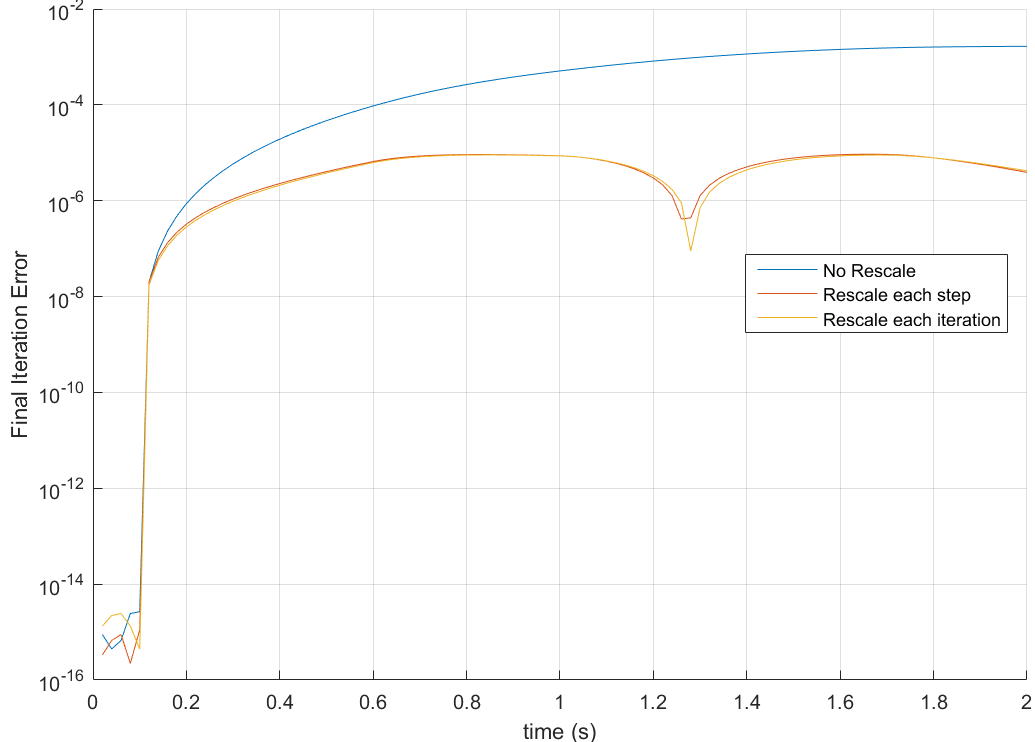
\includegraphics[width=\linewidth,height=3in,keepaspectratio]{figures/iter_error.png}
\end{figure}

\end{frame}
%-------------------------------------------------------------------

%-------------------------------------------------------------------
\begin{frame}{IQS converged error with analytical integration of precursors}

\begin{figure}
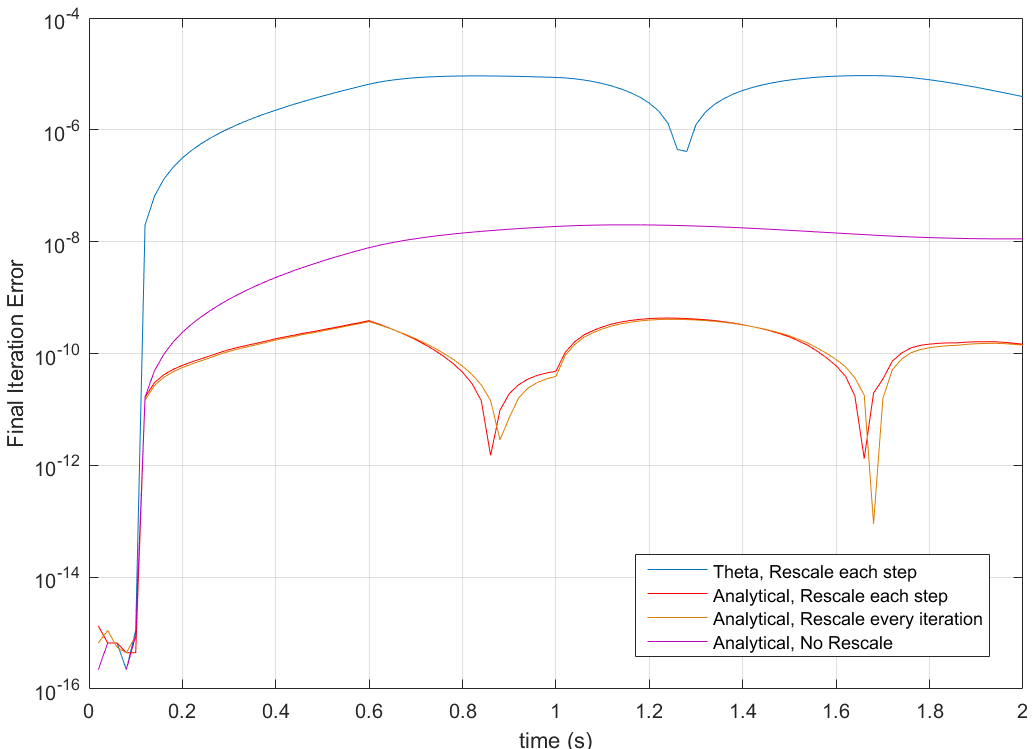
\includegraphics[width=\linewidth,height=3in,keepaspectratio]{figures/iter_error_an.png}
\end{figure}

\end{frame}
%-------------------------------------------------------------------

%-------------------------------------------------------------------
\begin{frame}{First and second order time step error convergence}

\begin{columns}
\column{\dimexpr\paperwidth-10pt}
\begin{figure}
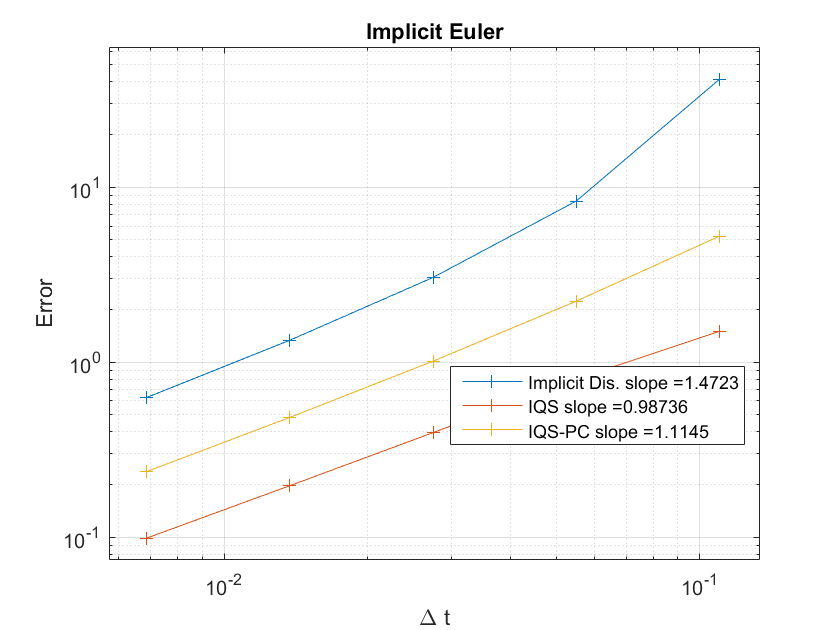
\includegraphics[width=0.5\linewidth]{figures/1D_conv_IE.png}
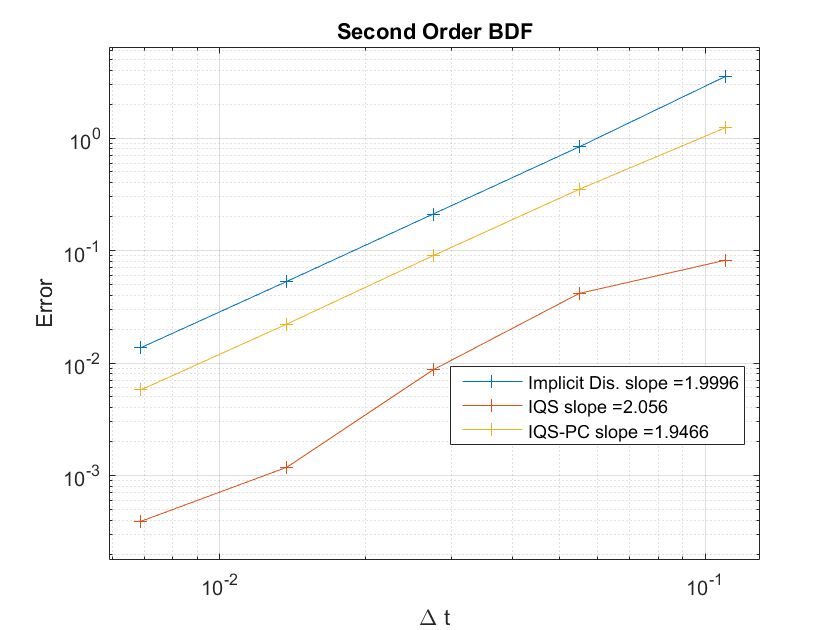
\includegraphics[width=0.5\linewidth]{figures/1D_conv_BDF2.png}
\end{figure}
\end{columns}

\end{frame}
%-------------------------------------------------------------------

%-------------------------------------------------------------------
\begin{frame}{Third and fourth order time step error convergence}

\begin{columns}
\column{\dimexpr\paperwidth-10pt}
\begin{figure}
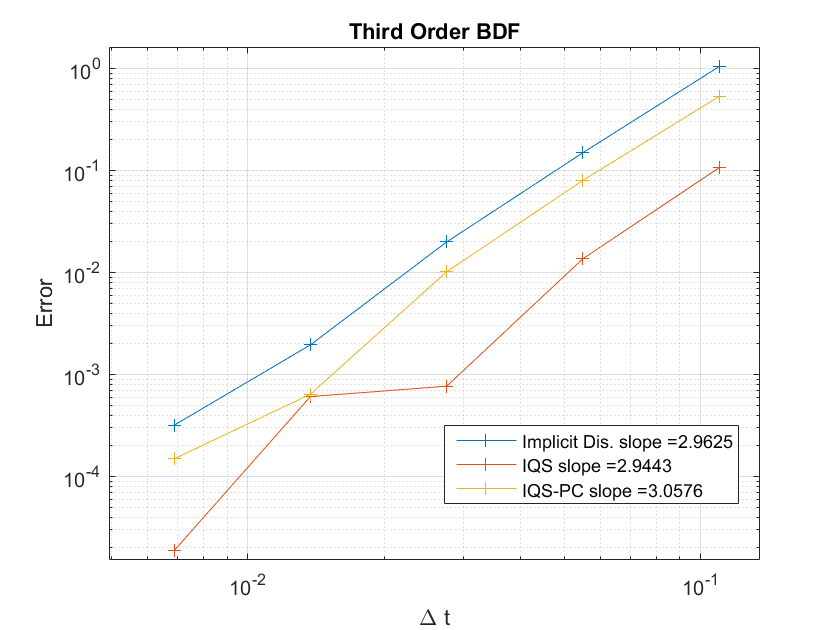
\includegraphics[width=0.5\linewidth]{figures/1D_conv_BDF3.png}
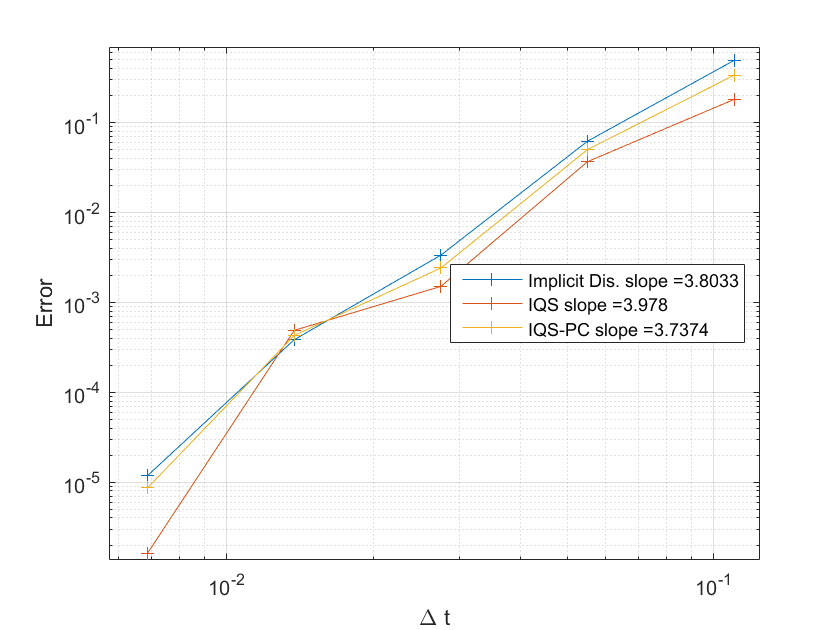
\includegraphics[width=0.5\linewidth]{figures/1D_conv_BDF4.png}
\end{figure}
\end{columns}

\end{frame}
%-------------------------------------------------------------------

%-------------------------------------------------------------------
\begin{frame}{SDIRK33 time step error convergence}

\begin{figure}
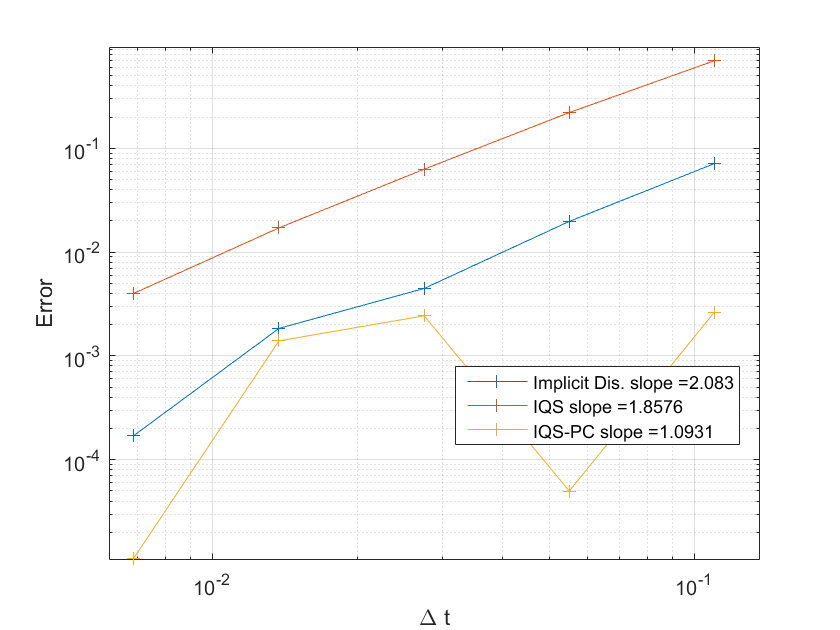
\includegraphics[width=\linewidth,height=3in,keepaspectratio]{figures/1D_conv_SDIRK33.png}
\end{figure}

\end{frame}
%-------------------------------------------------------------------

%-------------------------------------------------------------------
\begin{frame}{Rattlesnake time step error convergence}

\begin{columns}
\column{\dimexpr\paperwidth-10pt}
\begin{figure}
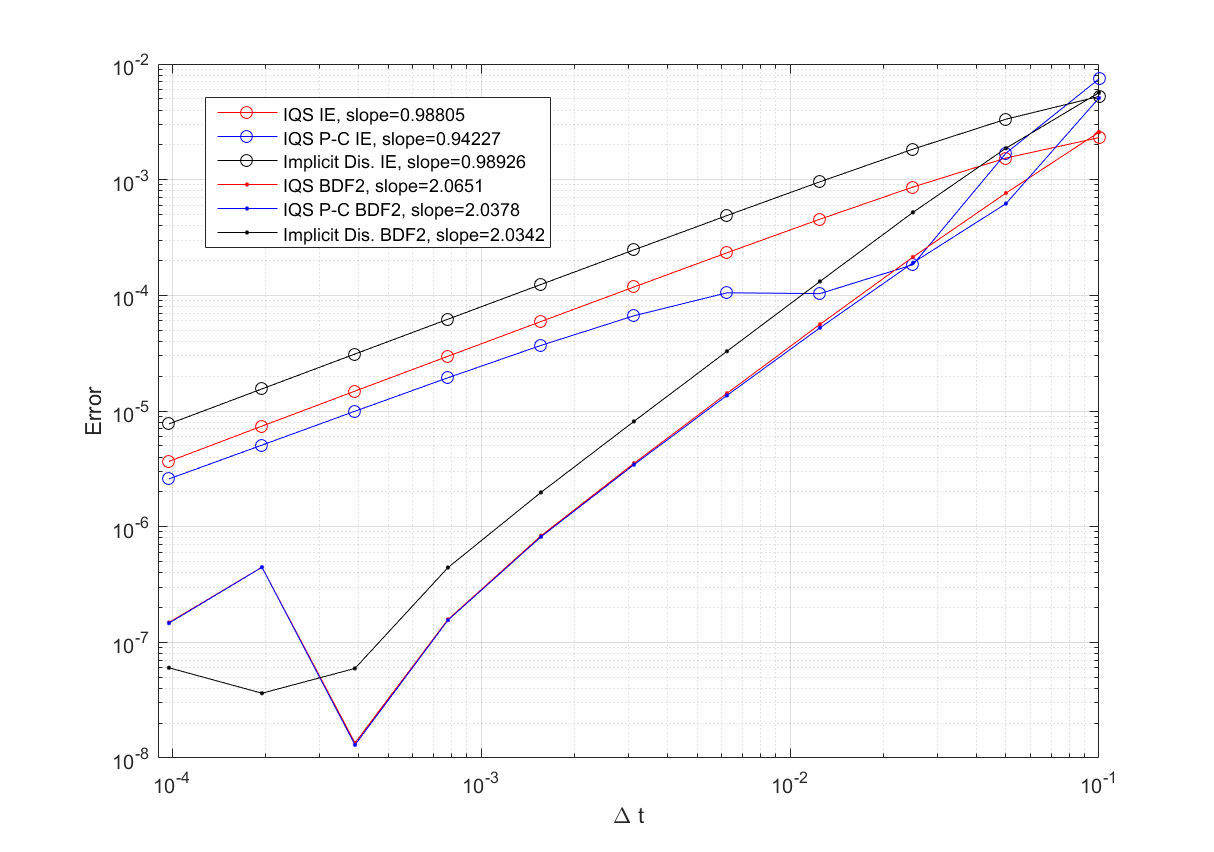
\includegraphics[width=0.5\paperwidth]{figures/1D_conv_Rat.png}
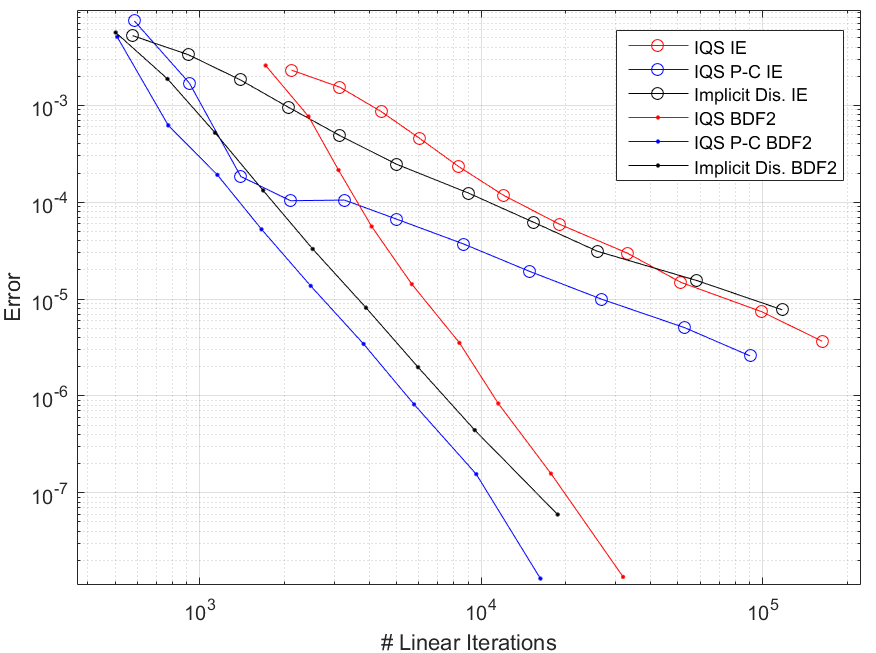
\includegraphics[width=0.5\paperwidth]{figures/1D_conv_lin.png}
\end{figure}
\end{columns}

\end{frame}
%-------------------------------------------------------------------

%------------------------------------------------------------------%
\subsection{TWIGL Benchmark}
%------------------------------------------------------------------%

%-------------------------------------------------------------------
\begin{frame}{TWIGL Benchmark}

\begin{columns}
\column{\dimexpr\paperwidth-10pt}
\begin{figure}
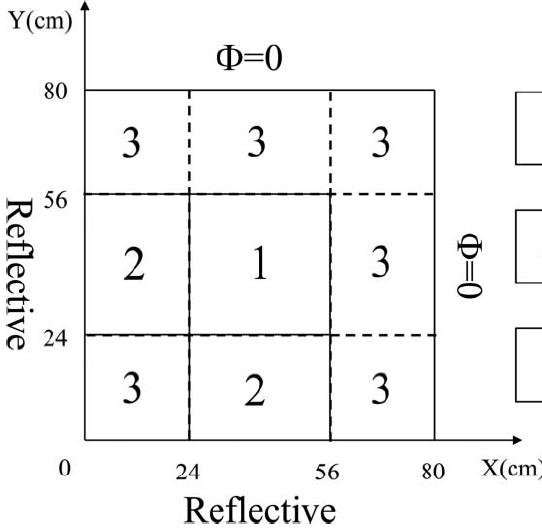
\includegraphics[width=0.5\linewidth]{figures/twigl_geom.png}
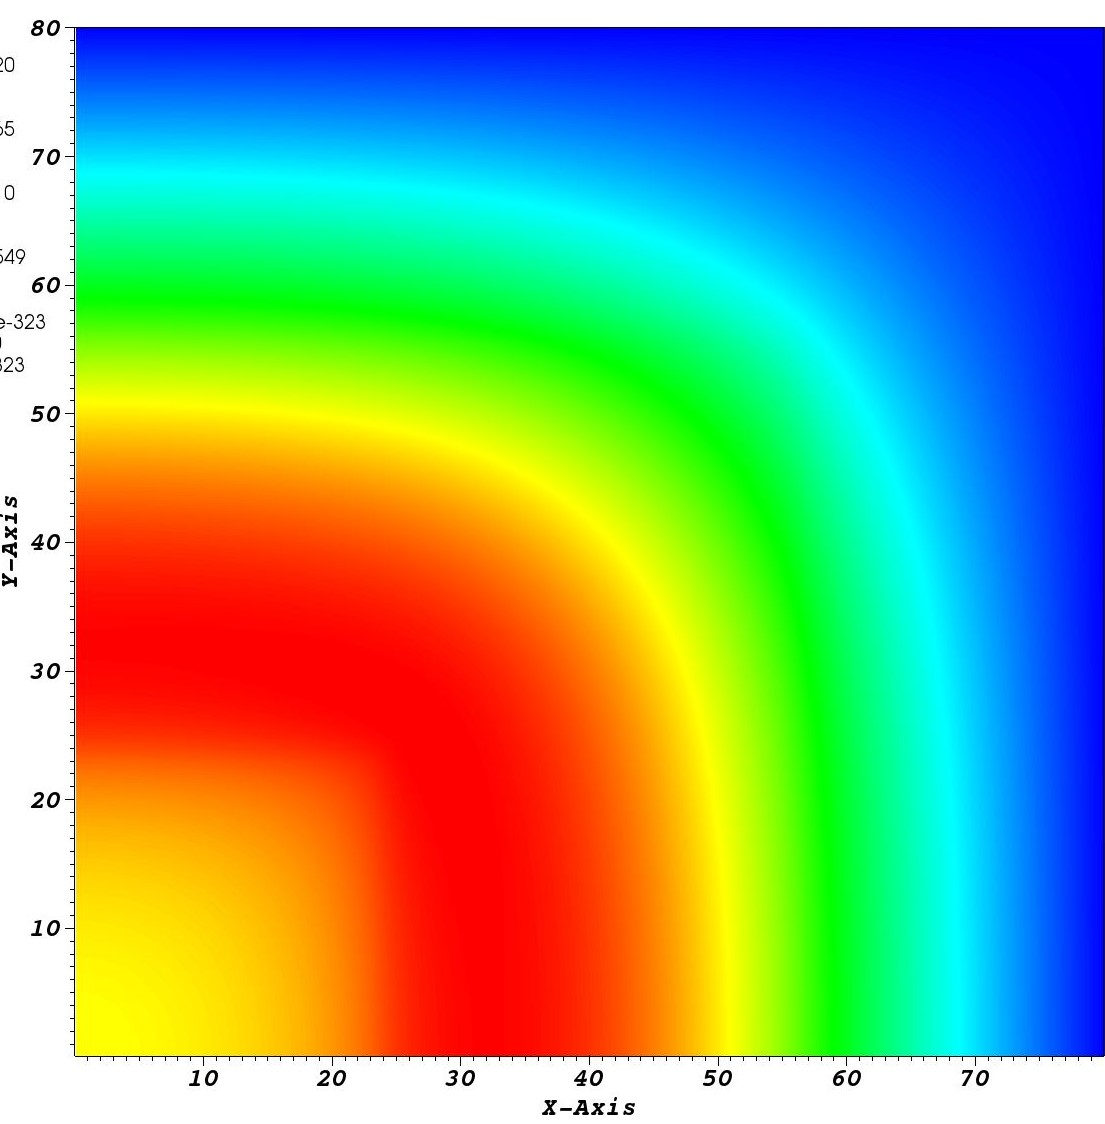
\includegraphics[width=0.5\linewidth]{figures/ndiff_ramp_flux.jpg}
\end{figure}
\end{columns}

\end{frame}
%-------------------------------------------------------------------

%-------------------------------------------------------------------
\begin{frame}{TWIGL Power Profile}

\begin{columns}

\column{.6\textwidth}
\begin{figure}
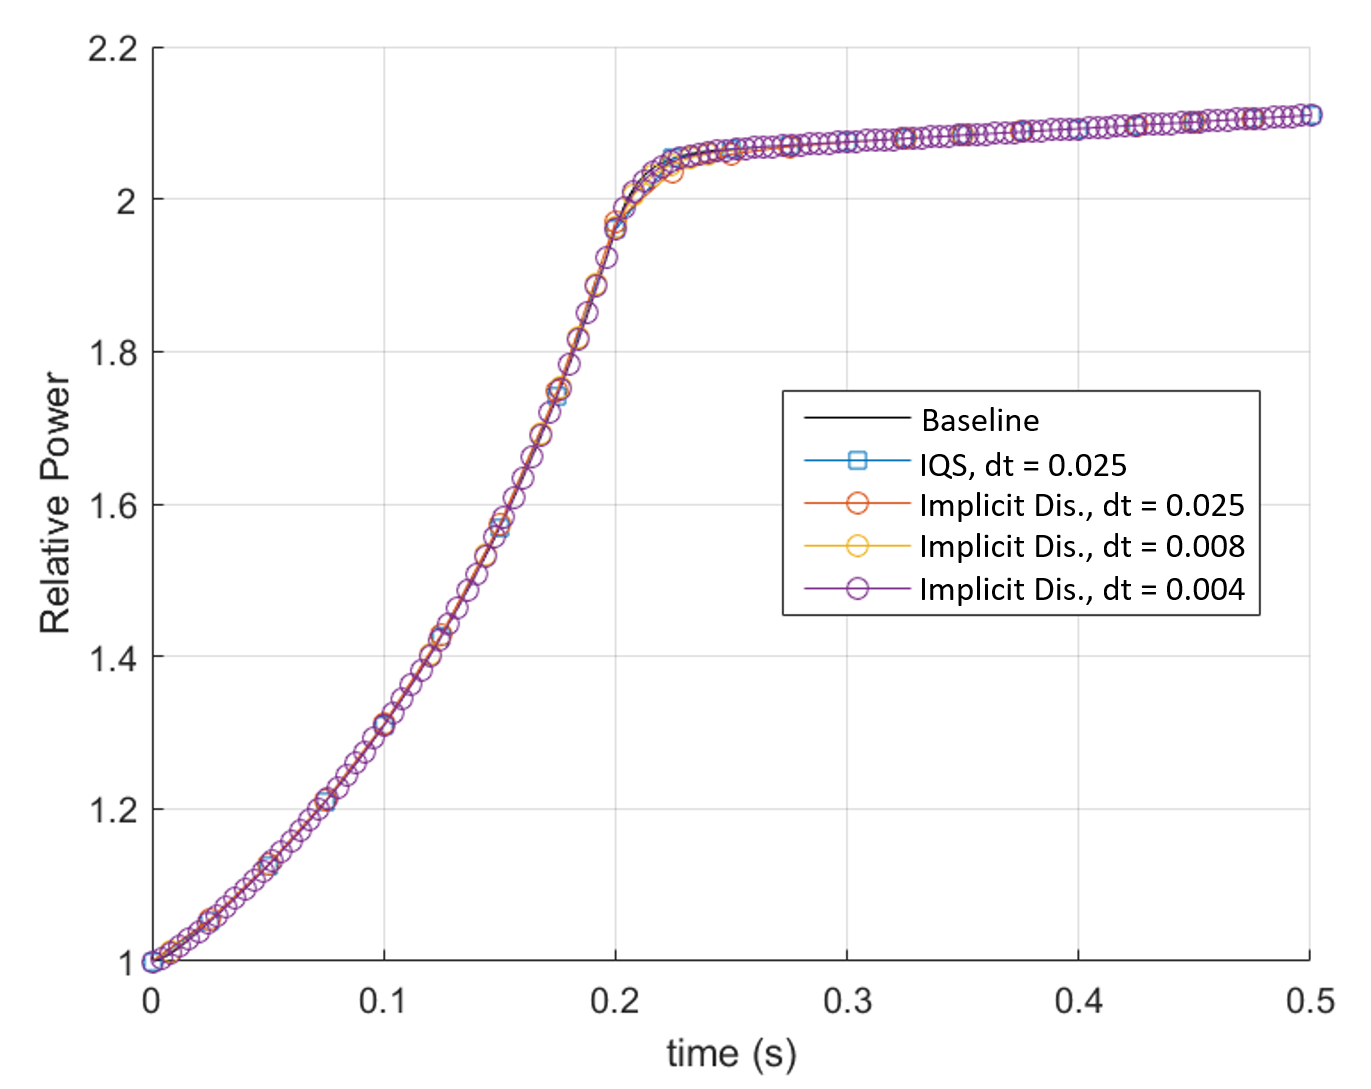
\includegraphics[width=\linewidth]{figures/TWIGL_power_plot.png}
\caption{TWIGL Power Profile}
\end{figure}

\column{.55\textwidth}
\begin{figure}
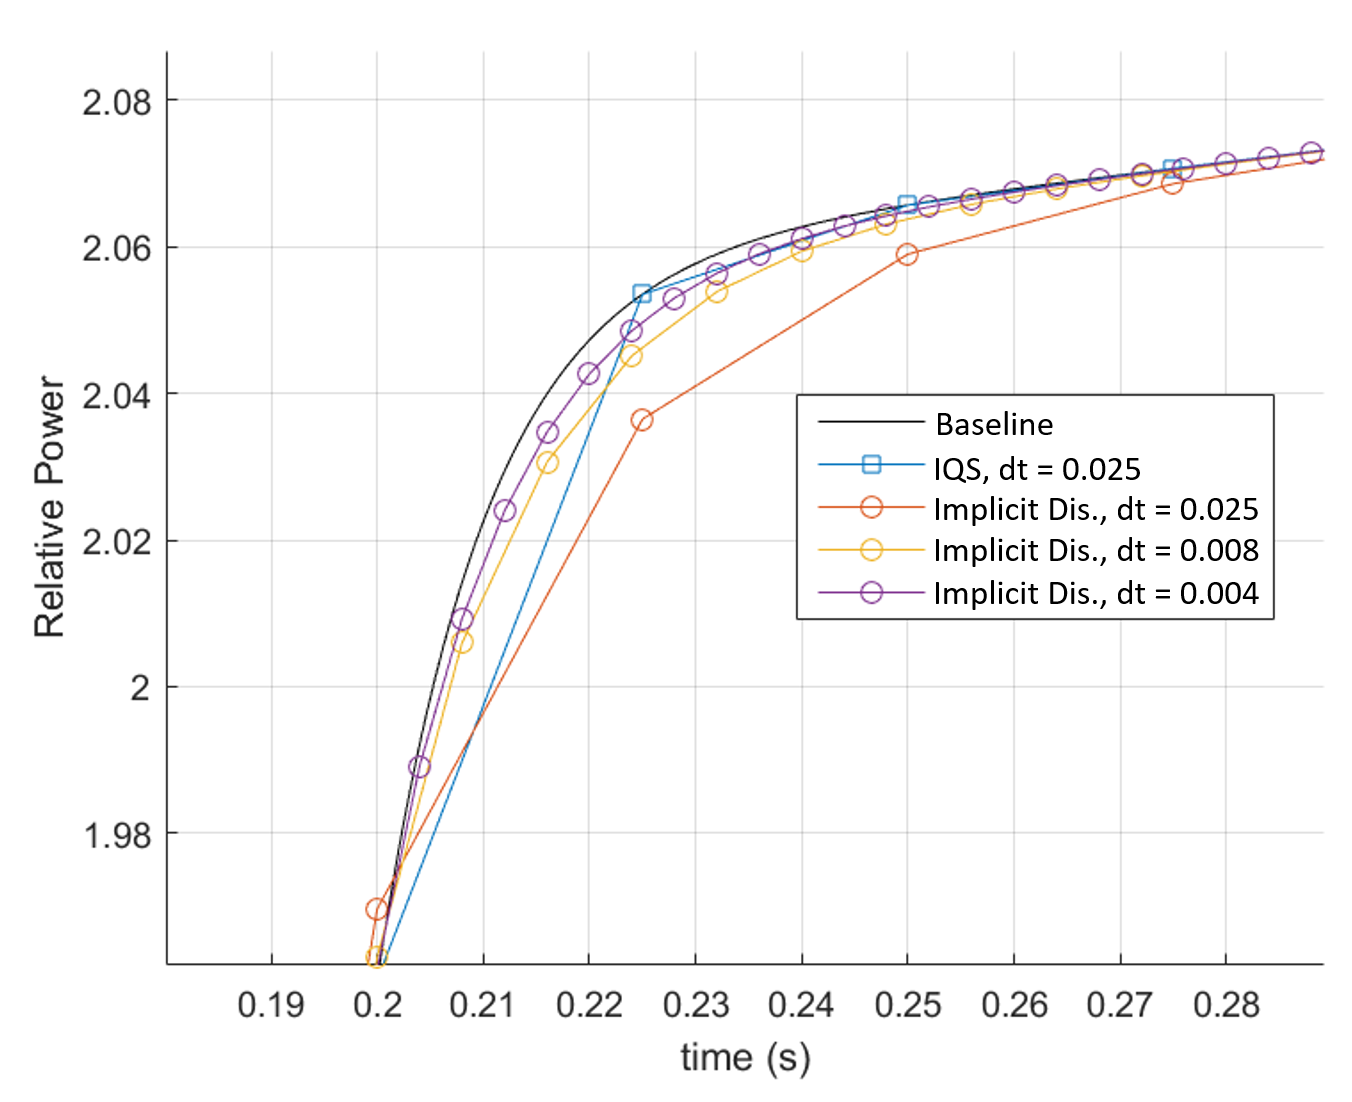
\includegraphics[width=\linewidth]{figures/TWIGL_power_plot2.png}
\caption{TWIGL Peak Power Profile}
\end{figure}

\end{columns}

\end{frame}
%-------------------------------------------------------------------

%-------------------------------------------------------------------
\begin{frame}{TWIGL time step error convergence}

\begin{columns}
\column{\dimexpr\paperwidth-10pt}
\begin{figure}
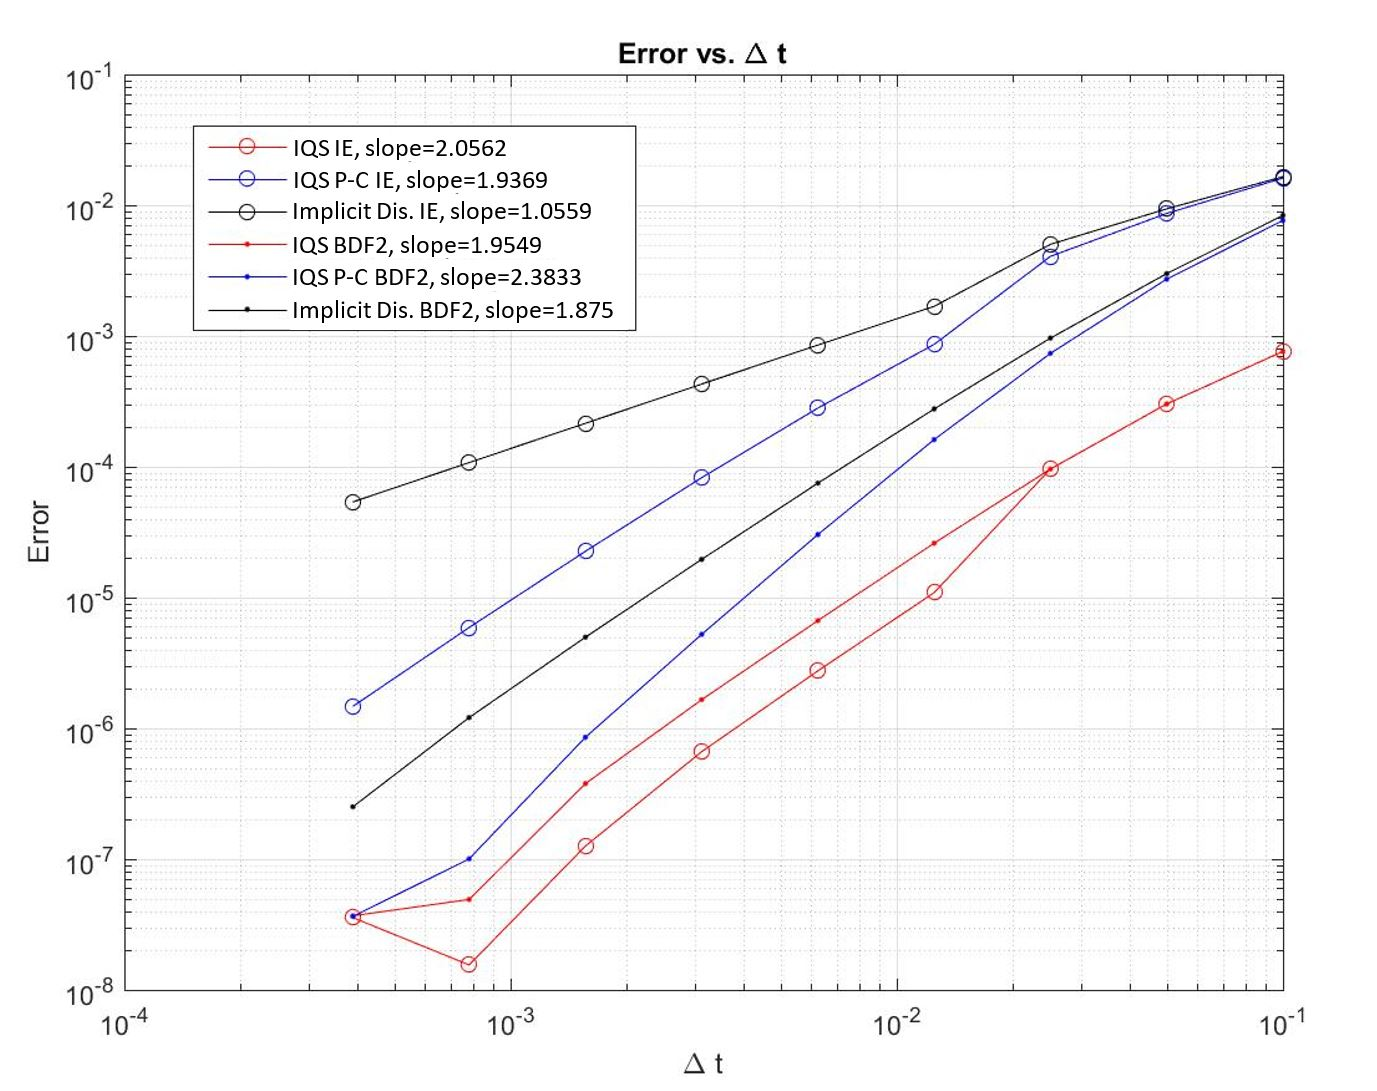
\includegraphics[width=0.5\linewidth]{figures/TWIGL_convergence.jpg}
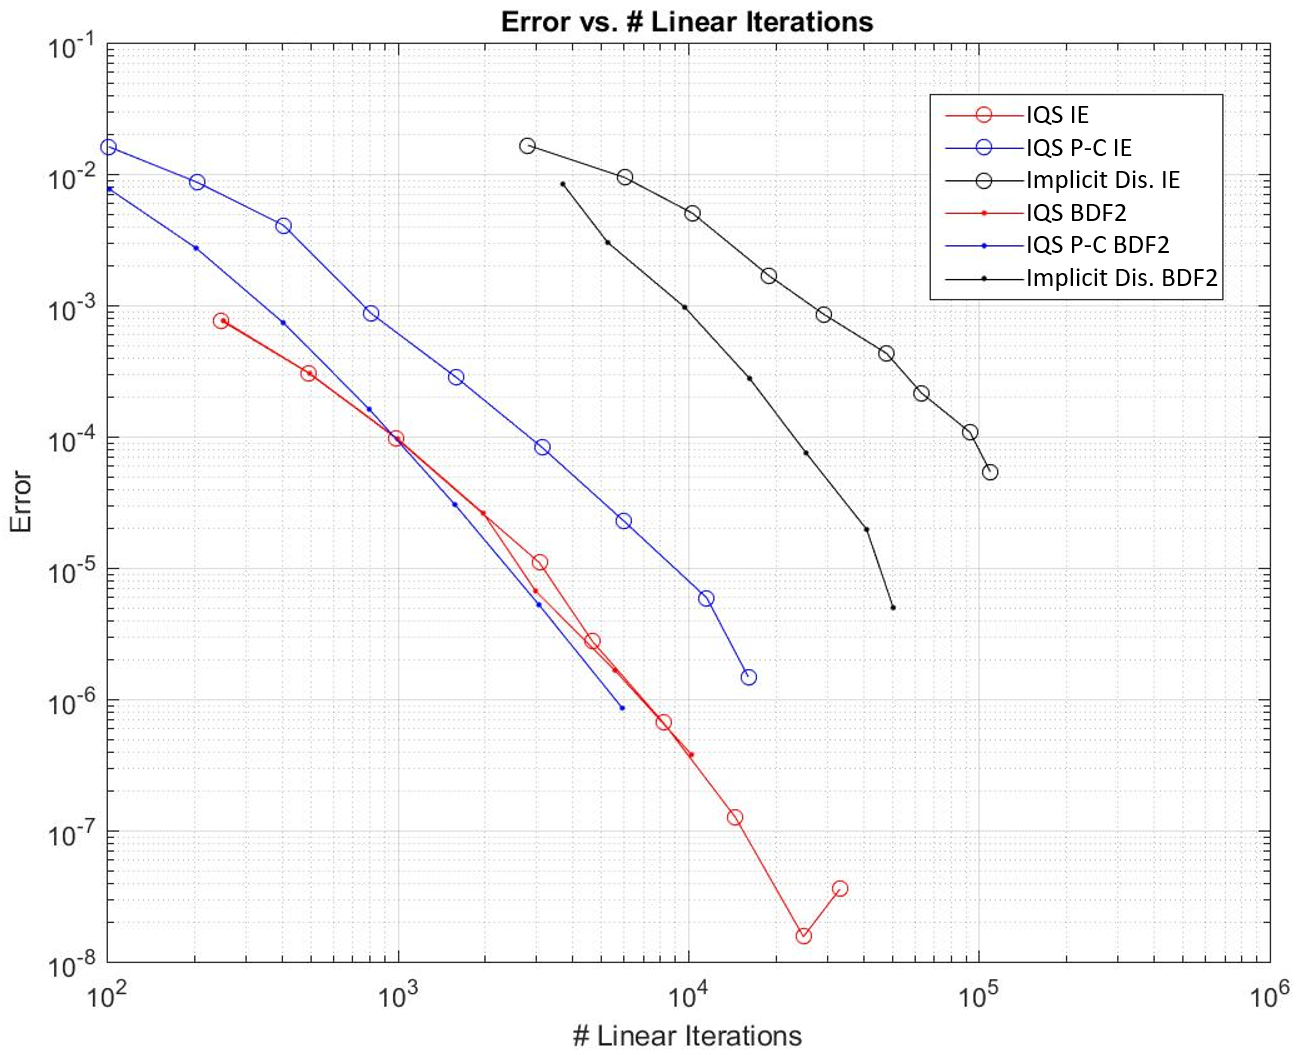
\includegraphics[width=0.5\linewidth]{figures/TWIGL_ramp_lin.png}
\end{figure}
\end{columns}

\end{frame}
%-------------------------------------------------------------------

%-------------------------------------------------------------------
\begin{frame}{TWIGL with Time Adaptation}

\begin{columns}

\column{.7\textwidth}
\begin{figure}
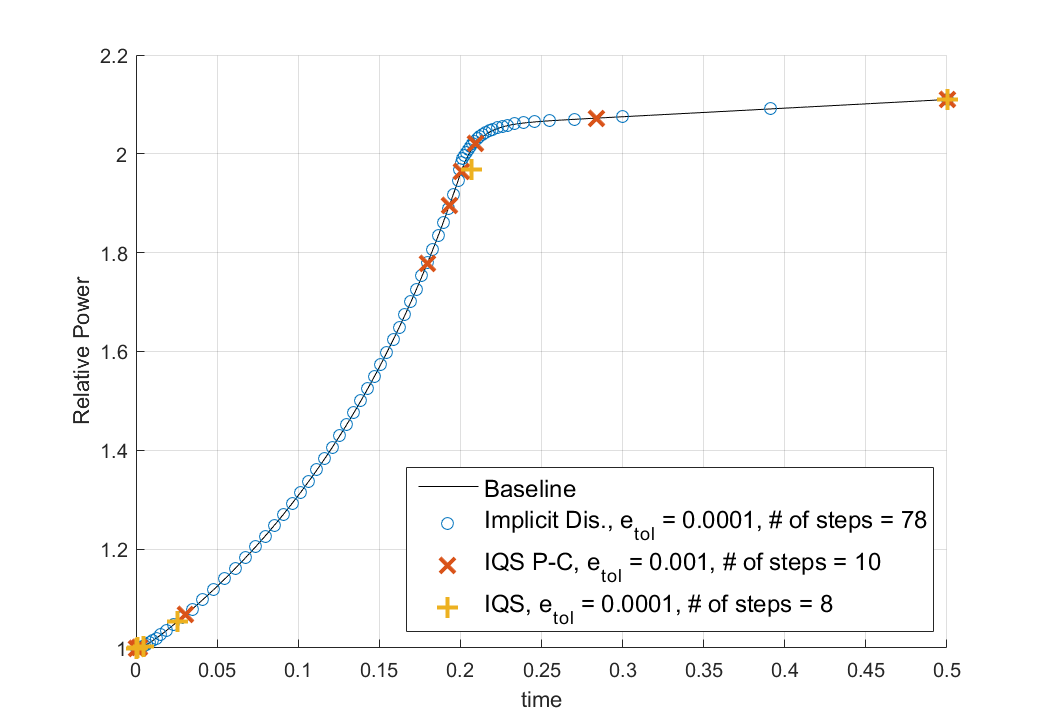
\includegraphics[width=\linewidth]{figures/TWIGL_power_plot_dt2.png}
\caption{TWIGL Power Profile}
\end{figure}

\column{.4\textwidth}
\begin{table}
\begin{center}
\colorbox{white}{\resizebox{\textwidth}{!}{
\begin{tabular}{|l|l|l|l|l|}
\hline
\multicolumn{5}{|c|}{Implicit Discretization}\\
\hline
Test & $e_{tol}$ & Error & Steps & Solves \\
\hline
1 &	0.05    &	0.00012677 &	9    &	29 \\
2 &	0.01    &	3.5555e-05 &	11   &	35 \\
3 &	0.005   &	4.0364e-05 &	11   &	31  \\
4 &	0.001   &	0.00294822 &	33   &	122  \\
5 &	0.0005  &	0.00099778 &	39   &	131  \\
\hline
\rowcolor{yellow} 6 &	0.0001  &	0.00019510 &	78   &	236  \\
\hline
7 &	5.0e-05 &	0.00018372 &	112  &	342  \\
8 &	1.0e-05 &	8.0564e-05 &	263  &	794 \\
\hline

\multicolumn{5}{|c|}{IQS} \\
\hline
Test & $e_{tol}$ & Error & Steps & Solves \\
\hline
1 &	0.05 	&	0.03380433 &	4   &	20   \\
2 &	0.01 	&	0.00166991 &	5   &	40  \\
3 &	0.005  	&	0.00886584 &	5   &	40  \\
4 &	0.001 	&	0.02976305 &	5   &	36  \\
5 &	0.0005 	&	0.00143781 &	6   &	55  \\
\hline
\rowcolor{yellow} 6 &	0.0001 	&	0.00016175 &	8   &	65  \\
\hline
7 &	5.0e-05 &	6.0328e-05 &	12  &	163  \\
8 &	1.0e-05 &	7.7103e-05 &	379 &	5729 \\
\hline

\multicolumn{5}{|c|}{IQS P-C} \\
\hline
Test & $e_{tol}$ & Error & Steps & Solves \\
\hline
1 &	0.05    &	0.03380433 &	4  &	9   \\
2 &	0.01    &	0.00263068 &	5  &	12  \\
3 &	0.005   &	0.00160486 &	6  &	21  \\
\hline
\rowcolor{yellow} 4 &	0.001   &	1.7527e-05 &	10 &	35  \\
\hline
5 &	0.0005  &	1.4185e-05 &	16 &	74  \\
6 &	0.0001  &	6.2903e-06 &	19 &	78  \\
7 &	5.0e-05 &	1.5247e-06 &	24 &	92  \\
8 &	1.0e-05  &	9.8321e-07 &	48 &	210 \\
\hline
\end{tabular}}}
\end{center}
\end{table}

\end{columns}

\end{frame}
%-------------------------------------------------------------------

%------------------------------------------------------------------%
\subsection{LRA Benchmark}
%------------------------------------------------------------------%

%-------------------------------------------------------------------
\begin{frame}{LRA Benchmark}
\begin{columns}

\column{0.6\textwidth}
\begin{figure}
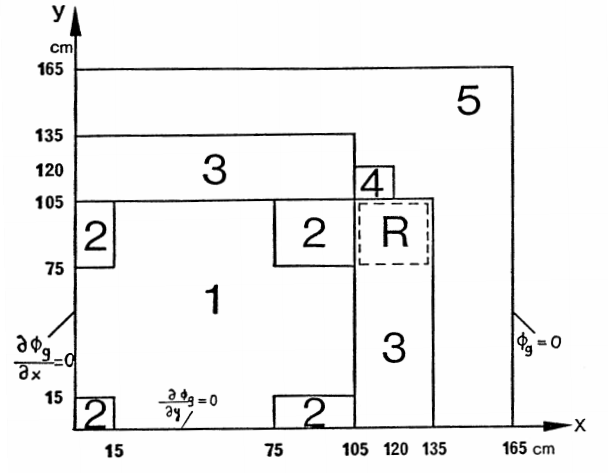
\includegraphics[width=\linewidth]{figures/lra.png}
\end{figure}

\column{0.6\textwidth}
\begin{figure}
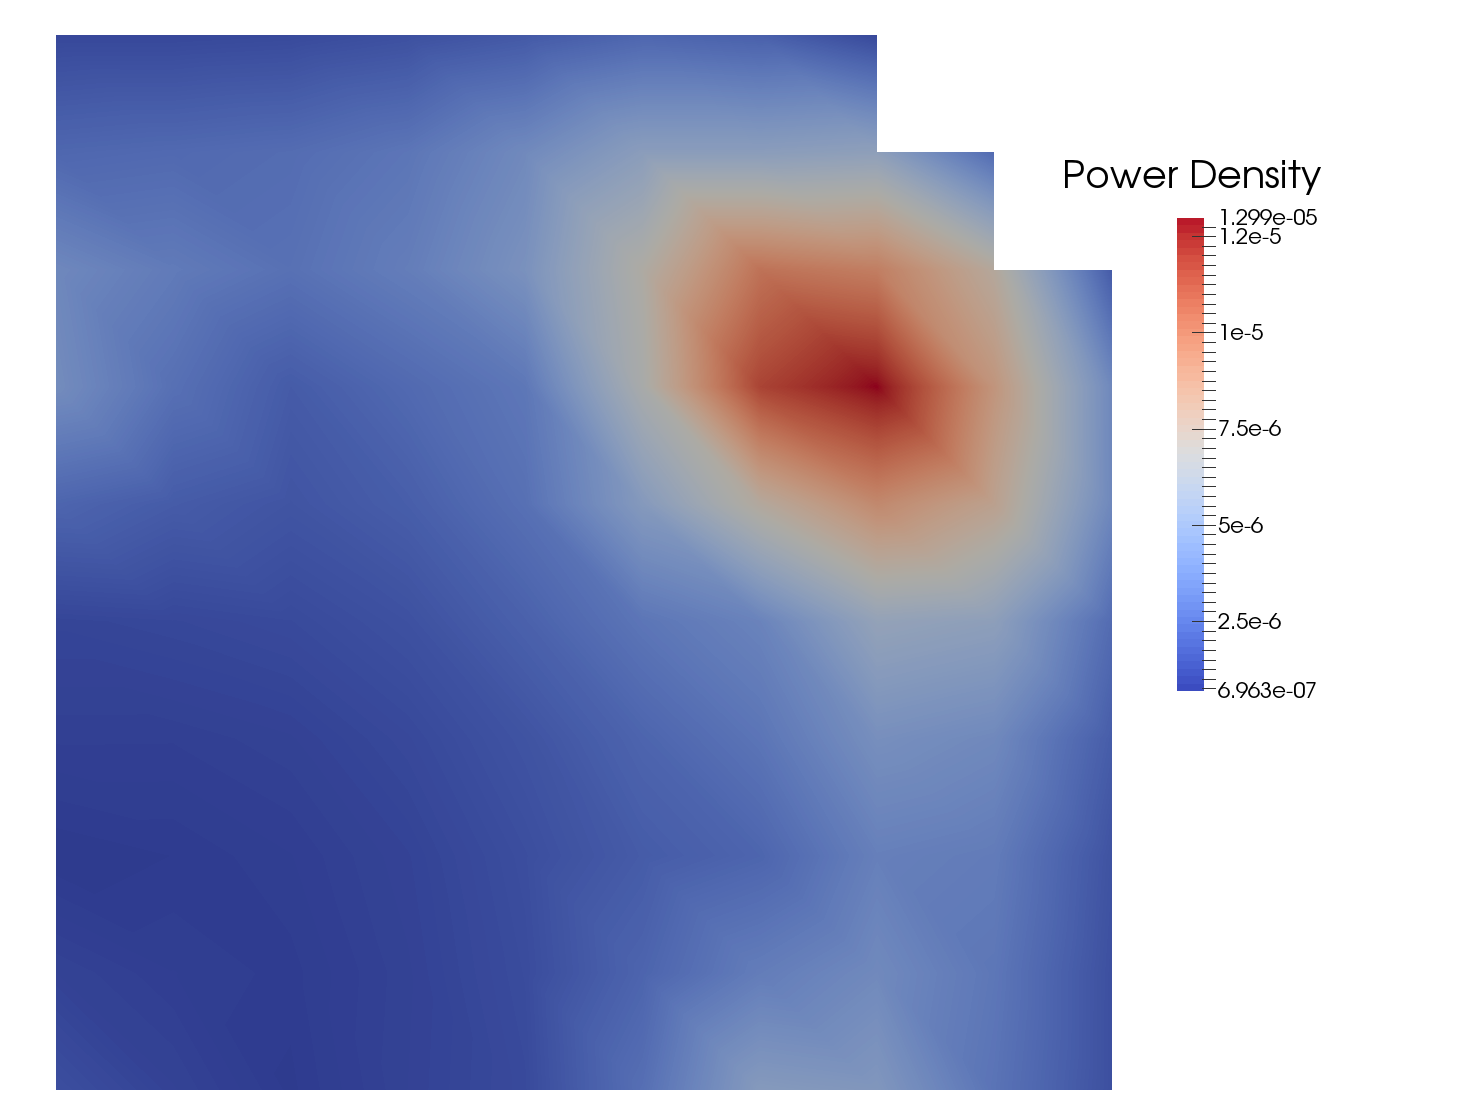
\includegraphics[width=\linewidth]{figures/lra_profile2D.png}
\end{figure}

\end{columns}
\end{frame}
%-------------------------------------------------------------------

%-------------------------------------------------------------------
\begin{frame}{LRA Power and Temperature Profile}

\begin{figure}
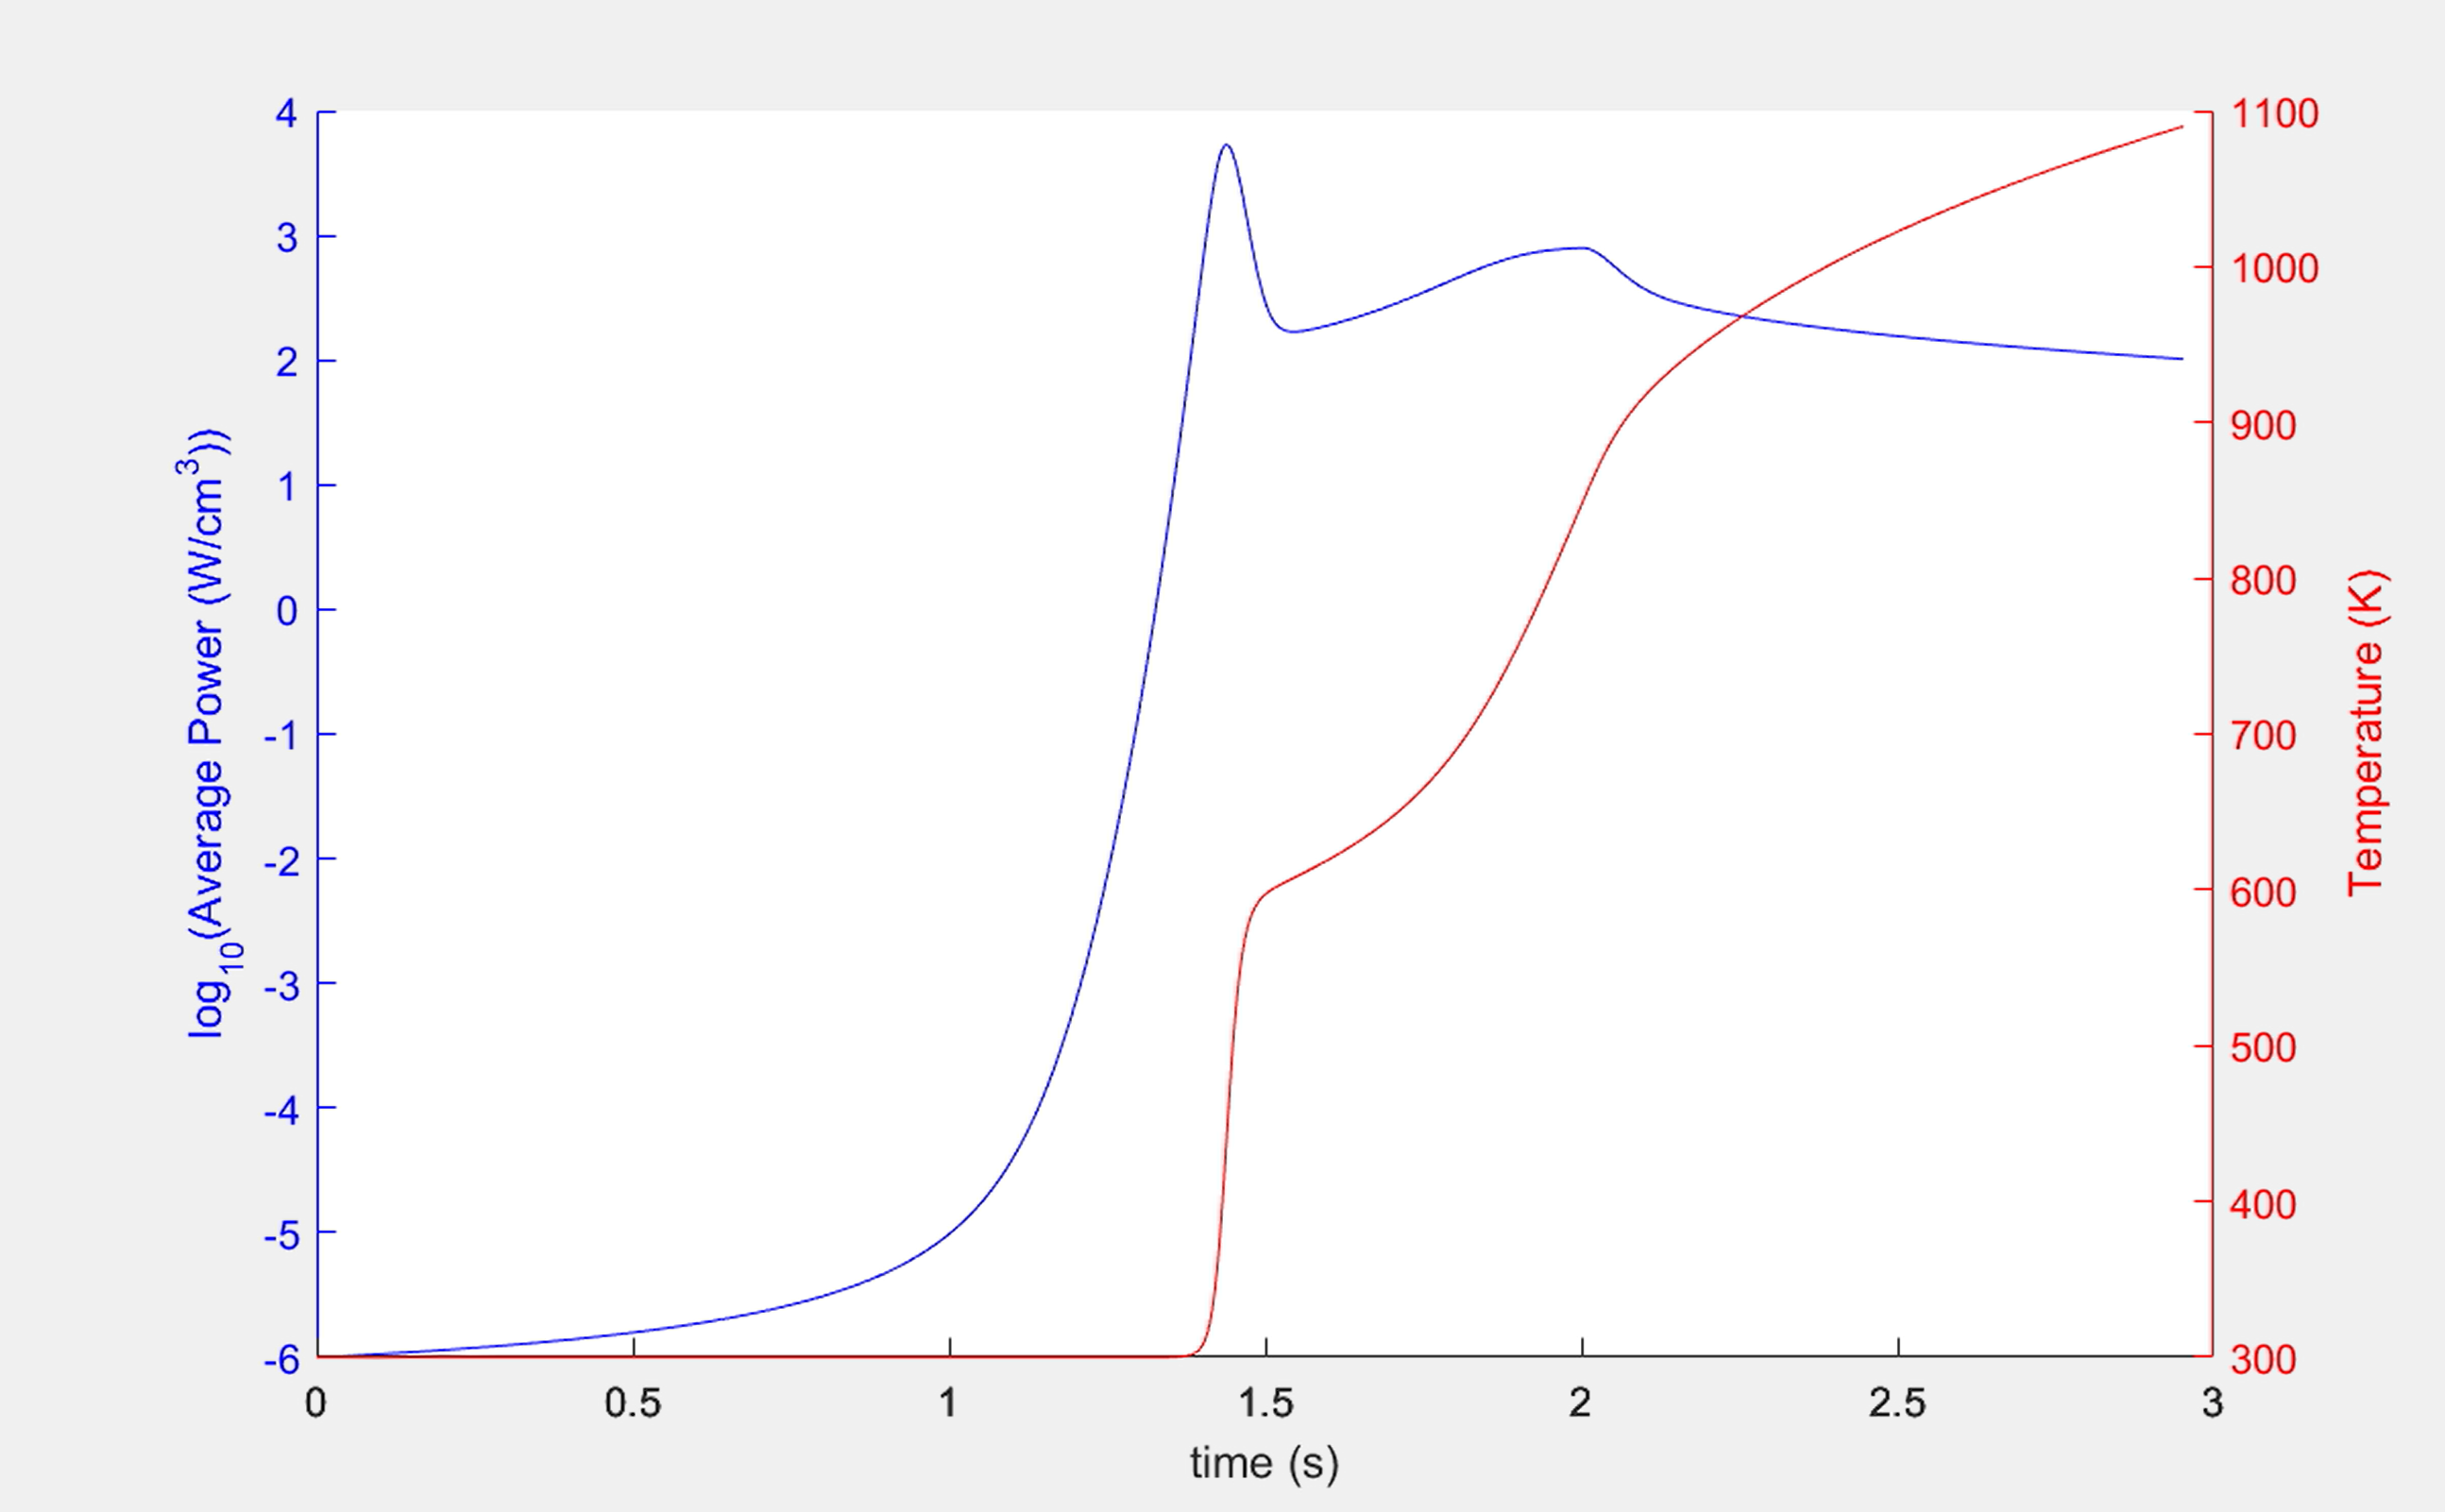
\includegraphics[width=\linewidth,height=3in,keepaspectratio]{figures/lra_profile.png}
\end{figure}

\end{frame}
%-------------------------------------------------------------------

%-------------------------------------------------------------------
\begin{frame}{LRA Time Step Error Convergence}
\begin{columns}

\column{0.6\textwidth}
\begin{figure}
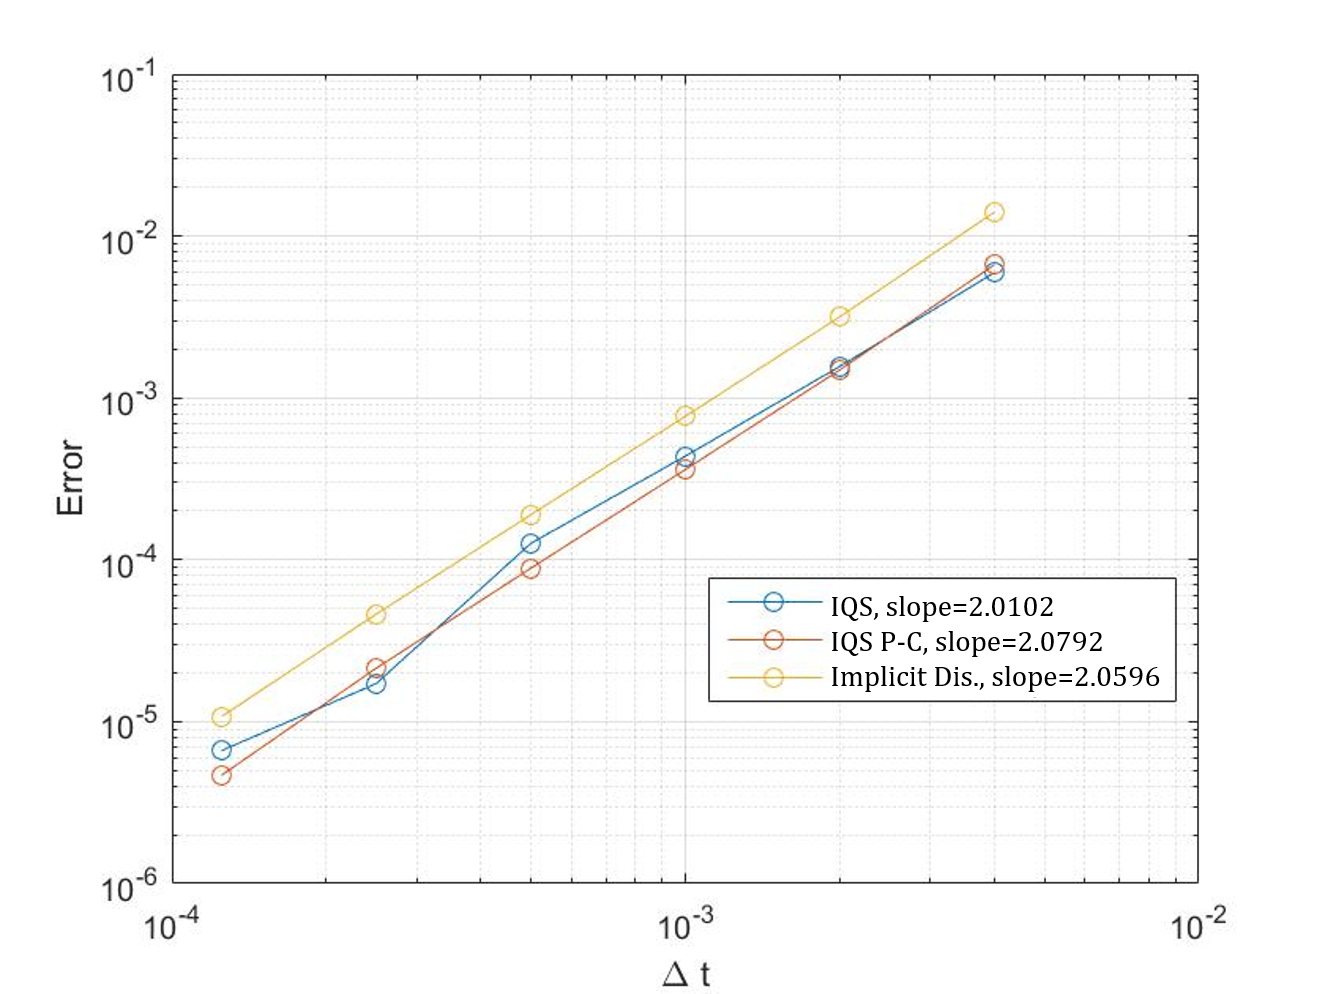
\includegraphics[width=\linewidth]{figures/lra_bad.png}
\caption{Only one temperature update per macro step}
\end{figure}

\column{0.6\textwidth}
\begin{figure}
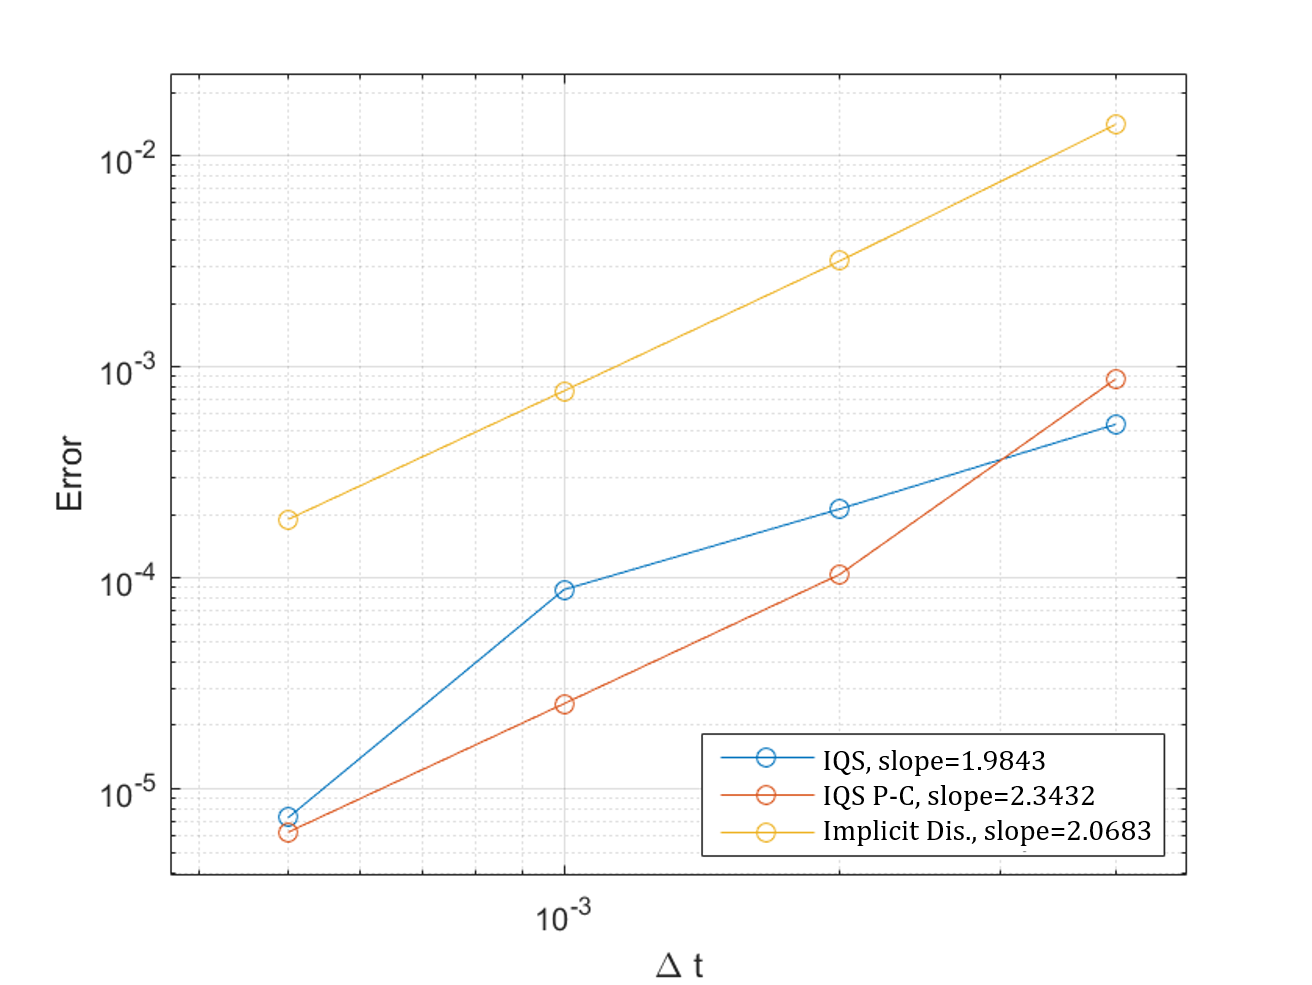
\includegraphics[width=\linewidth]{figures/lra_mp_convergence.png}
\caption{Five temperature updates per macro step}
\end{figure}

\end{columns}
\end{frame}
%-------------------------------------------------------------------

%-------------------------------------------------------------------
\begin{frame}{Analysis on Temperature Updates}

\begin{columns}

\column{.6\textwidth}
\begin{figure}
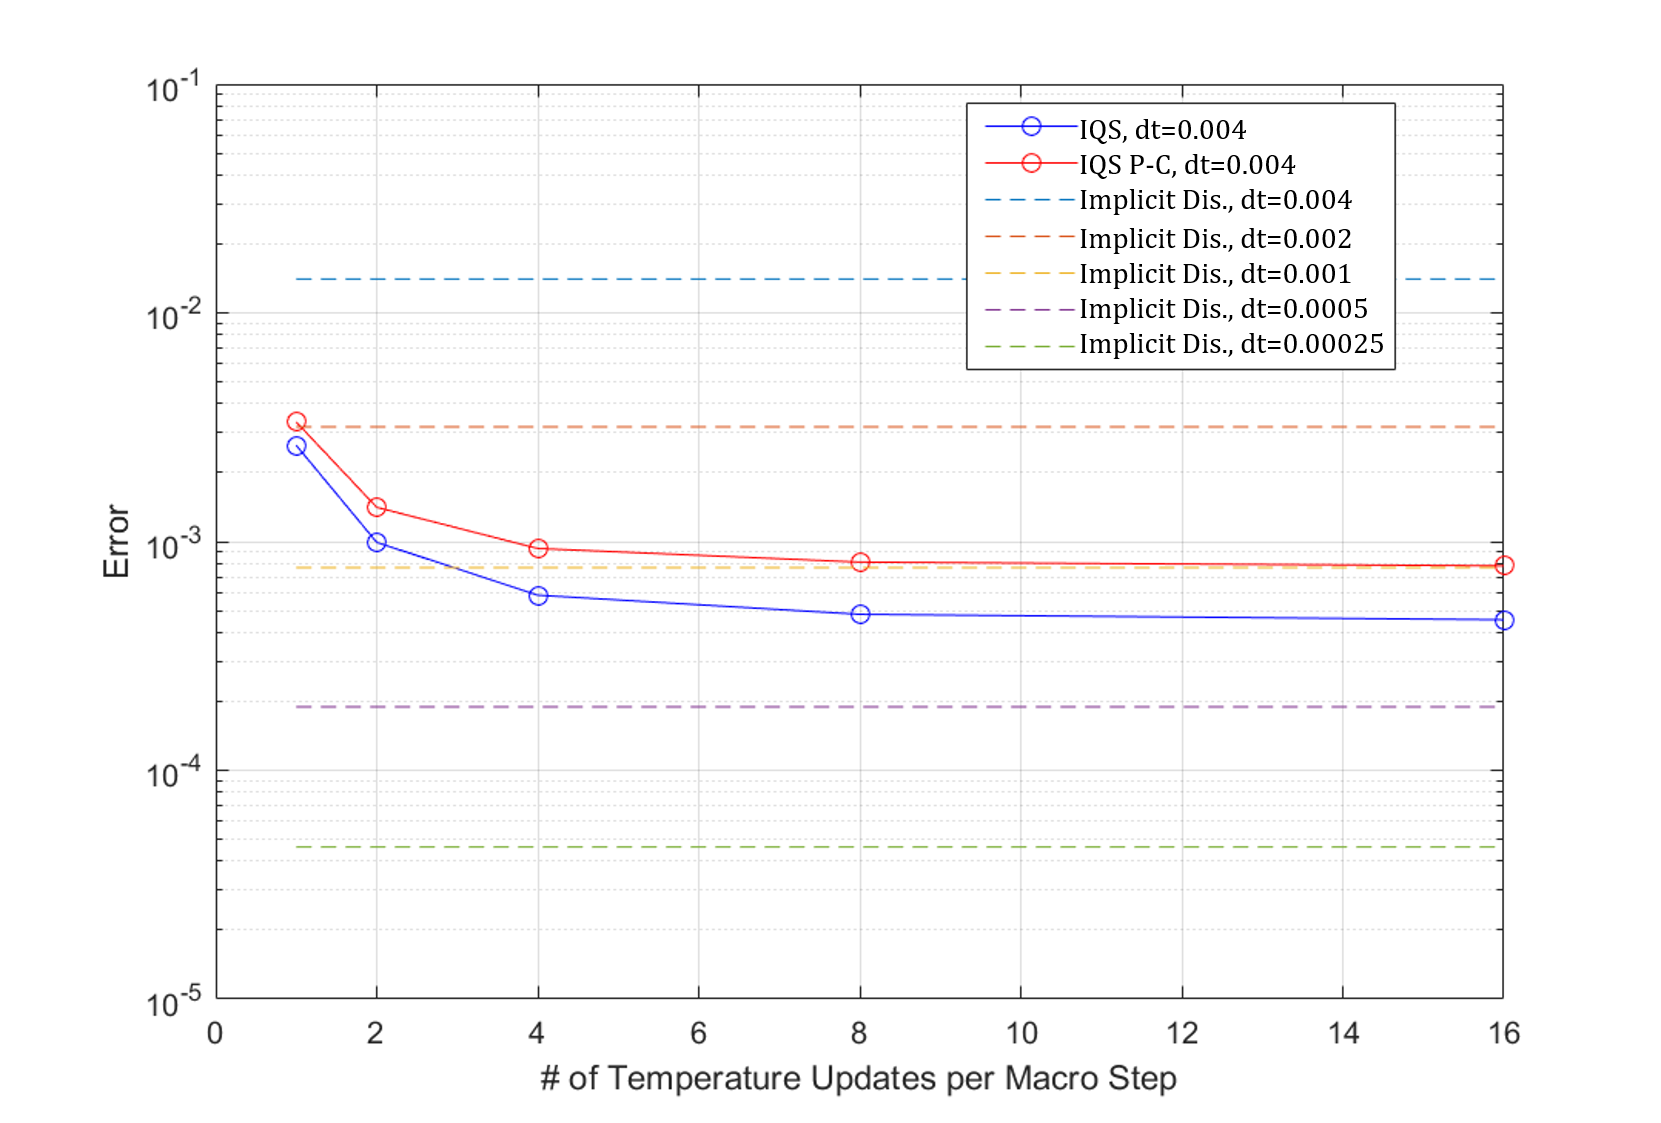
\includegraphics[width=\textwidth]{figures/lra_mp.png}
\end{figure}

\column{.5\textwidth}
\begin{table}
\captionsetup{font=scriptsize}
\begin{center}
\colorbox{white}{\resizebox{\textwidth}{!}{
\begin{tabular}{|l|l|ccc|}
\hline
\multicolumn{5}{|c|}{Implicit Discretization}\\
\hline
Run  &  $\Delta t$ & Error & Runtime (hr) & Linear Iter.\\
\hline
1	& 4.0e-3	& 1.407e-2 	& 4.11	& 7.13e4	\\
2	& 2.0e-3	& 3.174e-3 	& 6.01	& 9.49e4 	\\
3 	& 1.0e-3 	& 7.690e-4 	& 10.38	& 1.45e5	\\
4 	& 5.0e-4 	& 1.892e-4 	& 21.91	& 2.08e5	\\
5 	& 2.5e-4	& 4.590e-5 	& 25.23	& 3.16e5	\\
\hline
\end{tabular}}}
\end{center}
\end{table}
\vspace{-7mm}

\begin{table}
\captionsetup{font=small}
\begin{center}
\colorbox{white}{\resizebox{\textwidth}{!}{
\begin{tabular}{|l|l|ccc|}
\hline
\multicolumn{5}{|c|}{IQS}\\
\hline
	&  Temperature 	&  		& Runtime 	& \% Increase	\\
Run	&  Updates 	& Error & (hr)		& in Runtime$^*$\\
\hline
1	& 1		& 2.612e-3 	& 3.96 	& -3.18\%	\\
2	& 2		& 9.893e-4 	& 6.02	&  47.1\%	\\
3 	& 4 	& 5.796e-4 	& 7.87	&  92.3\%	\\
4 	& 8 	& 4.772e-4 	& 12.61	& 207.9\% 	\\
5 	& 16	& 4.516e-4 	& 22.14	& 440.7\%	\\
\hline
\end{tabular}}}
\end{center}
\end{table}
\vspace{-7mm}

\begin{table}
\captionsetup{font=scriptsize}
\begin{center}
\colorbox{white}{\resizebox{\textwidth}{!}{
\begin{tabular}{|l|l|ccc|}
\hline
\multicolumn{5}{|c|}{IQS P-C}\\
\hline
	&  Temperature 	&  		& Runtime 	& \% Increase	\\
Run	&  Updates 	& Error & (hr)		& in Runtime$^*$\\
\hline
1	& 1		& 3.488e-3 	& 2.91 	& -28.9\%	\\
2	& 2		& 1.349e-3 	& 3.73	& -9.00\%	\\
3 	& 4 	& 9.161e-4 	& 3.97	& -3.04\%	\\
4 	& 8 	& 8.052e-4 	& 5.39	&  31.7\%	\\
5 	& 16	& 7.905e-4 	& 8.19	&  100\%	\\
\hline
\end{tabular}}}
%}
\\
\tiny $^*$ runtime difference from $\Delta t = 0.004$ implicit dis.
\end{center}
\end{table}

\end{columns}

\end{frame}
%-------------------------------------------------------------------

%-------------------------------------------------------------------
\begin{frame}{LRA Dynamical Time Scale Analysis}

\begin{figure}
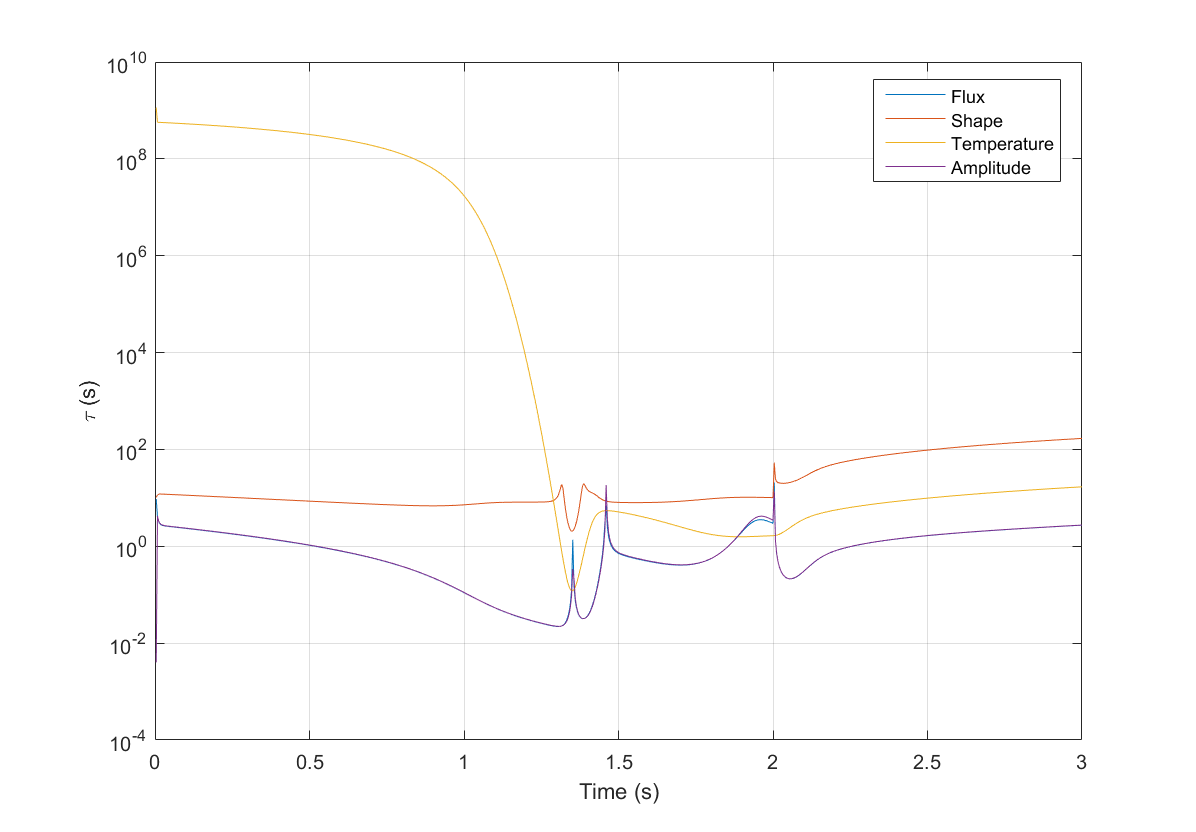
\includegraphics[width=\linewidth,height=3in,keepaspectratio]{figures/time_constant_lra.png}
\end{figure}

\end{frame}
%-------------------------------------------------------------------

%-------------------------------------------------------------------
\begin{frame}{LRA with Time Adaptation}

\begin{columns}

\column{.6\textwidth}
\begin{figure}
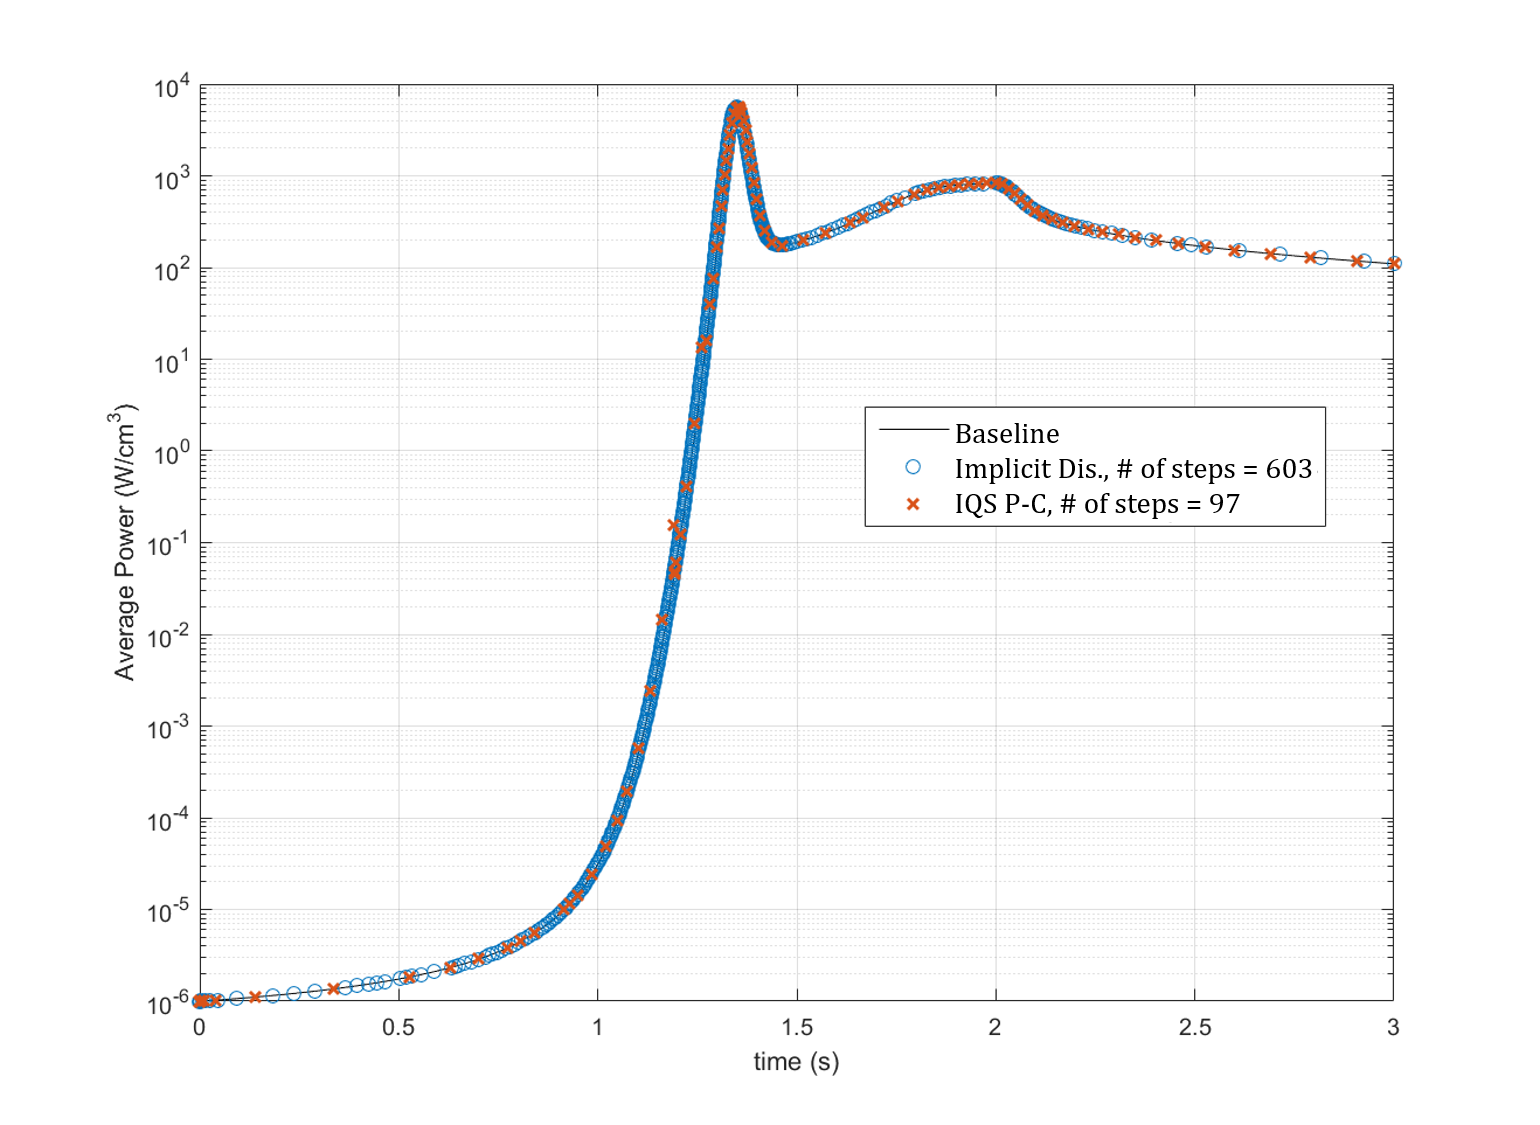
\includegraphics[width=\linewidth]{figures/LRA_DT2.png}
\caption{LRA Power Profile}
\end{figure}

\column{.6\textwidth}
\begin{figure}
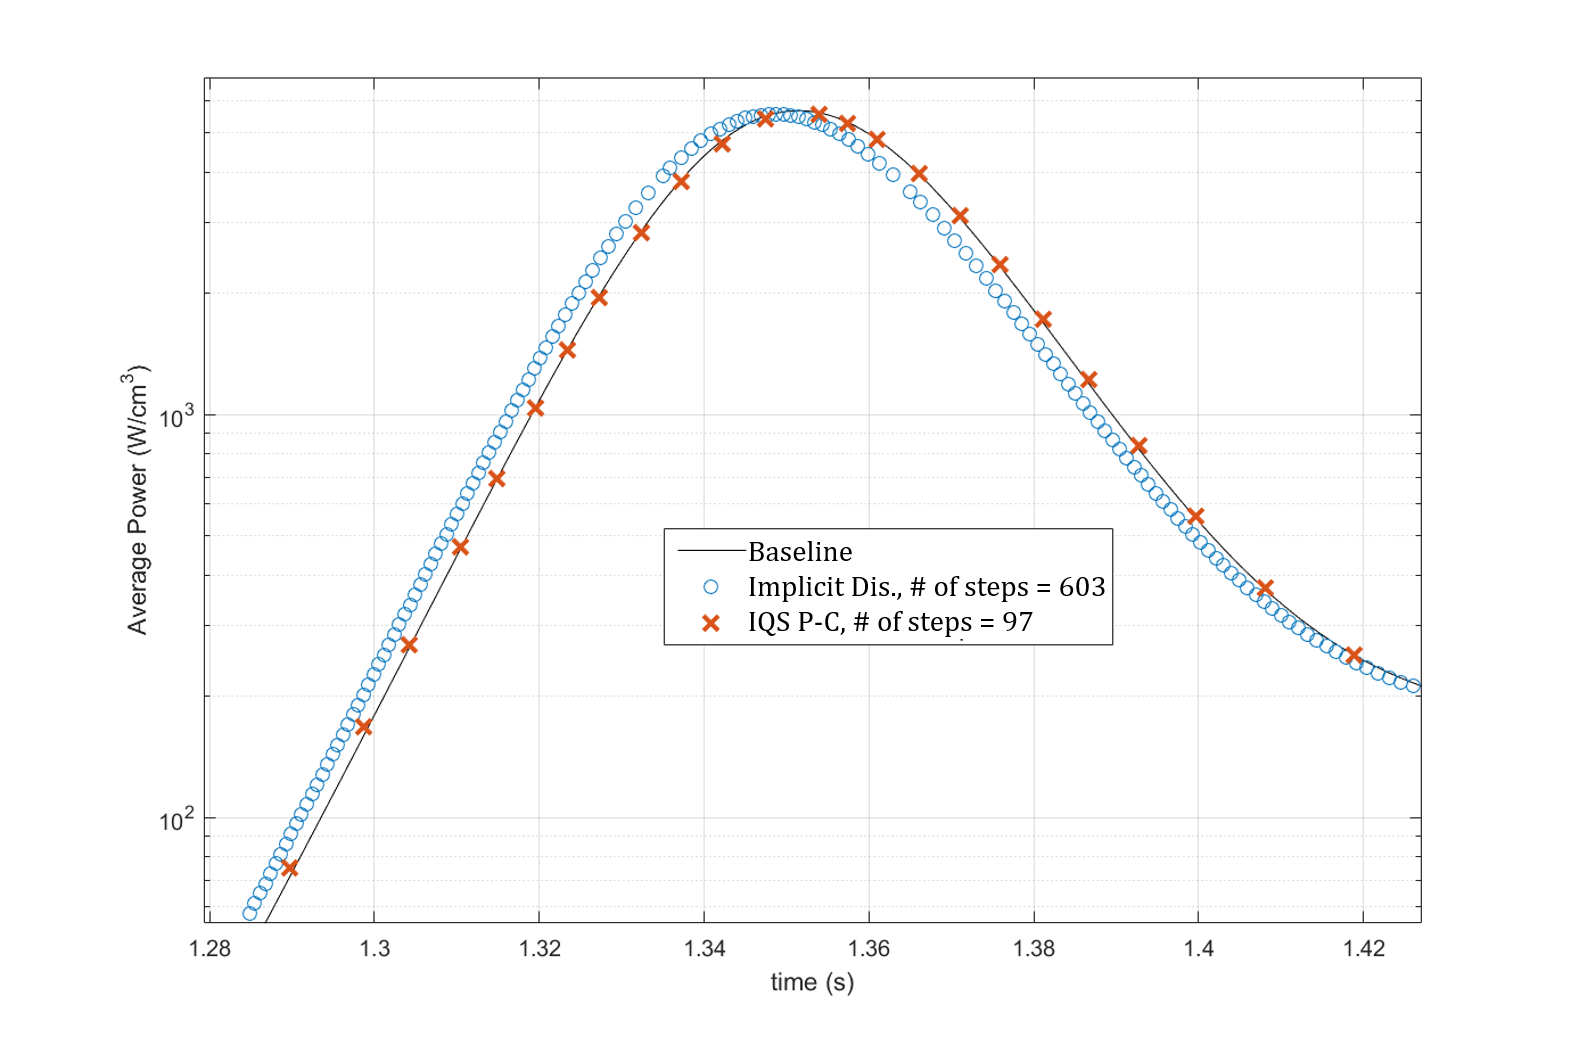
\includegraphics[width=\linewidth]{figures/LRA_DT2_peak.png}
\caption{LRA Peak Power Profile}
\end{figure}

\end{columns}

\begin{table}
\begin{center}
\resizebox{\textwidth}{!}{
\begin{tabular}{|l|l|l|l|l|l|l|}
\hline
 & \multicolumn{3}{|c|}{Brute Force} & \multicolumn{3}{|c|}{IQS P-C} \\
\hline
Event & Power (W/cm$^3$) & Error & Steps & Power (W/cm$^3$) & Error & Steps \\
\hline
Max Power & 5567.3 & 0.019454 & 423 & 5568.3 & 0.019274 & 47 \\
End (3 s) & 109.66 & 2.3650e-4 & 603 & 109.65 & 3.0622e-4 & 97 \\
\hline
\end{tabular}}
\end{center}
\end{table}

\end{frame}
%-------------------------------------------------------------------

%------------------------------------------------------------------%
\subsection{TREAT Transient-15}
%------------------------------------------------------------------%

%-------------------------------------------------------------------
\begin{frame}{TREAT: Transient-15 Example}
\begin{columns}

\column{0.6\textwidth}
\begin{figure}
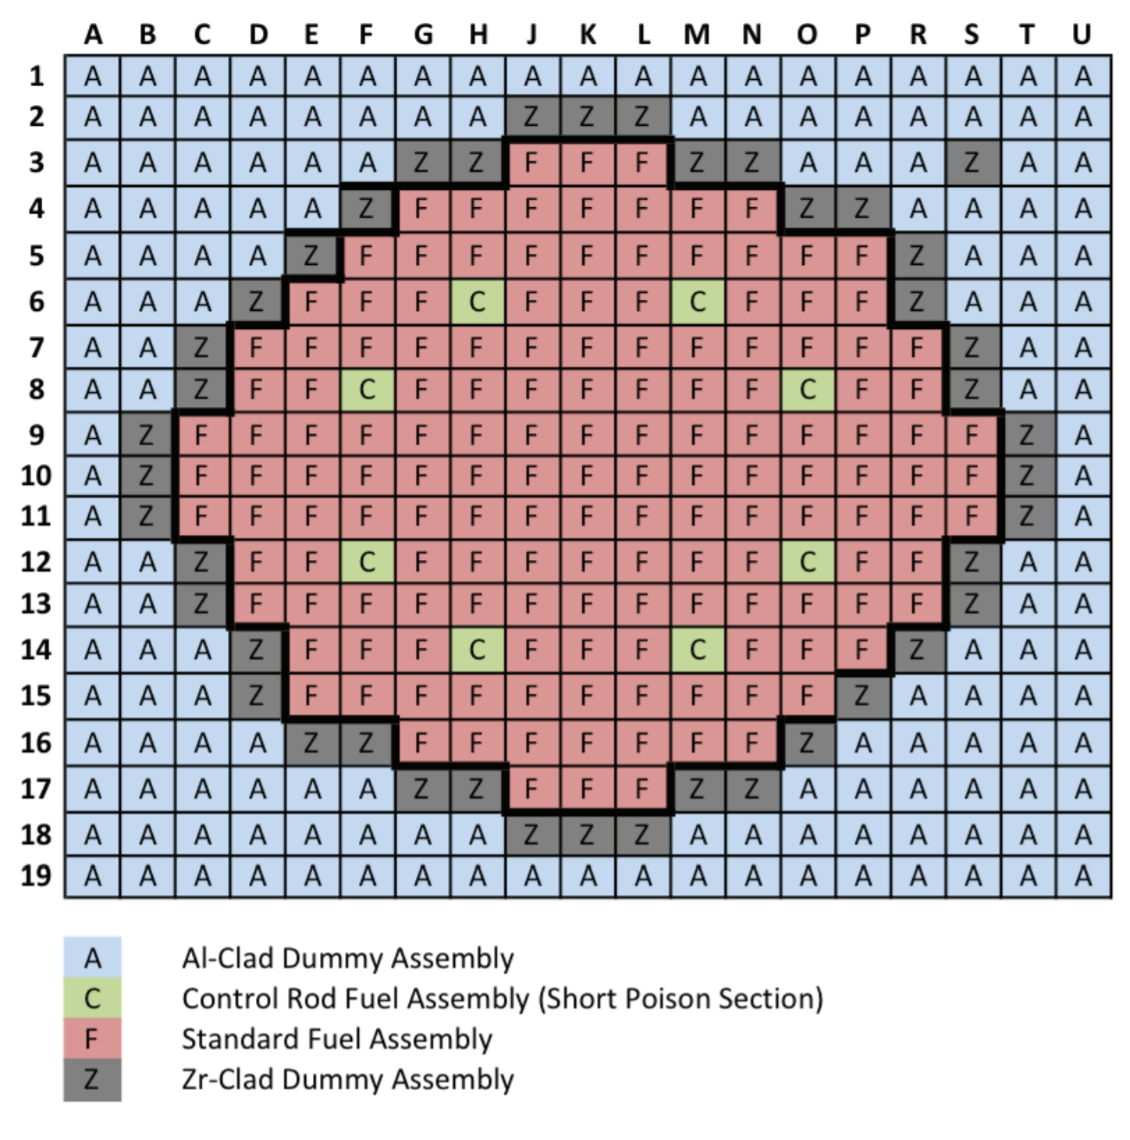
\includegraphics[width=\linewidth]{figures/Tran15_config.png}
\end{figure}

\column{0.5\textwidth}
\begin{figure}
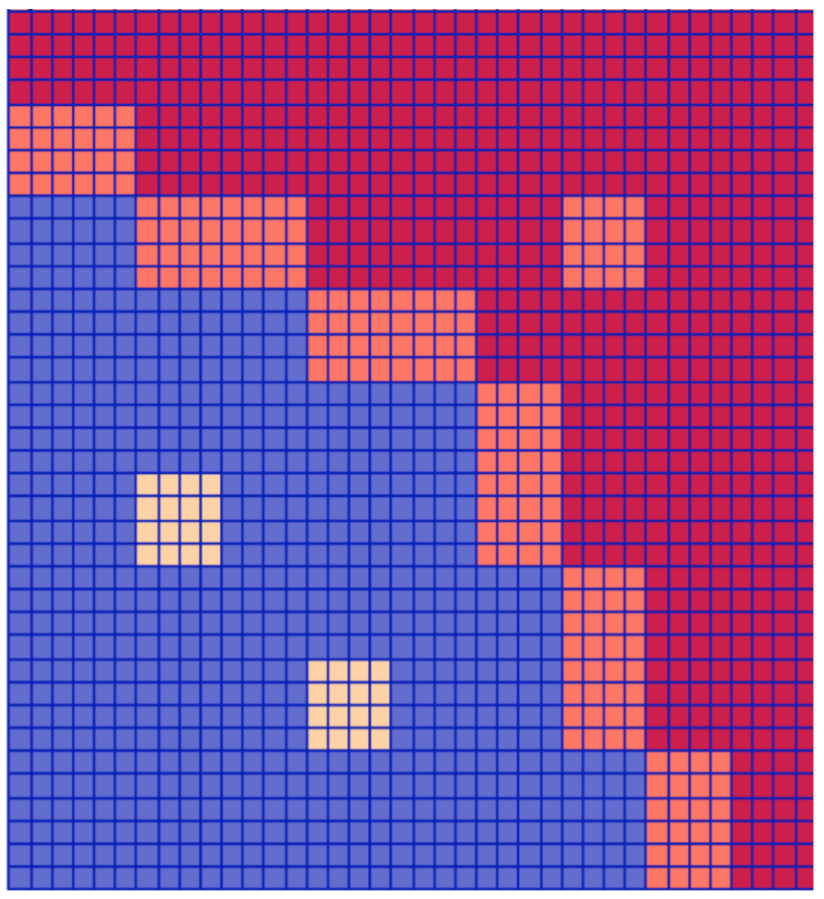
\includegraphics[width=\linewidth]{figures/Tran15_mesh_homo.png}
\end{figure}

\end{columns}
\end{frame}
%-------------------------------------------------------------------

%-------------------------------------------------------------------
\begin{frame}{Transient-15 Power Profile}
\begin{columns}

\column{0.6\textwidth}
\begin{figure}
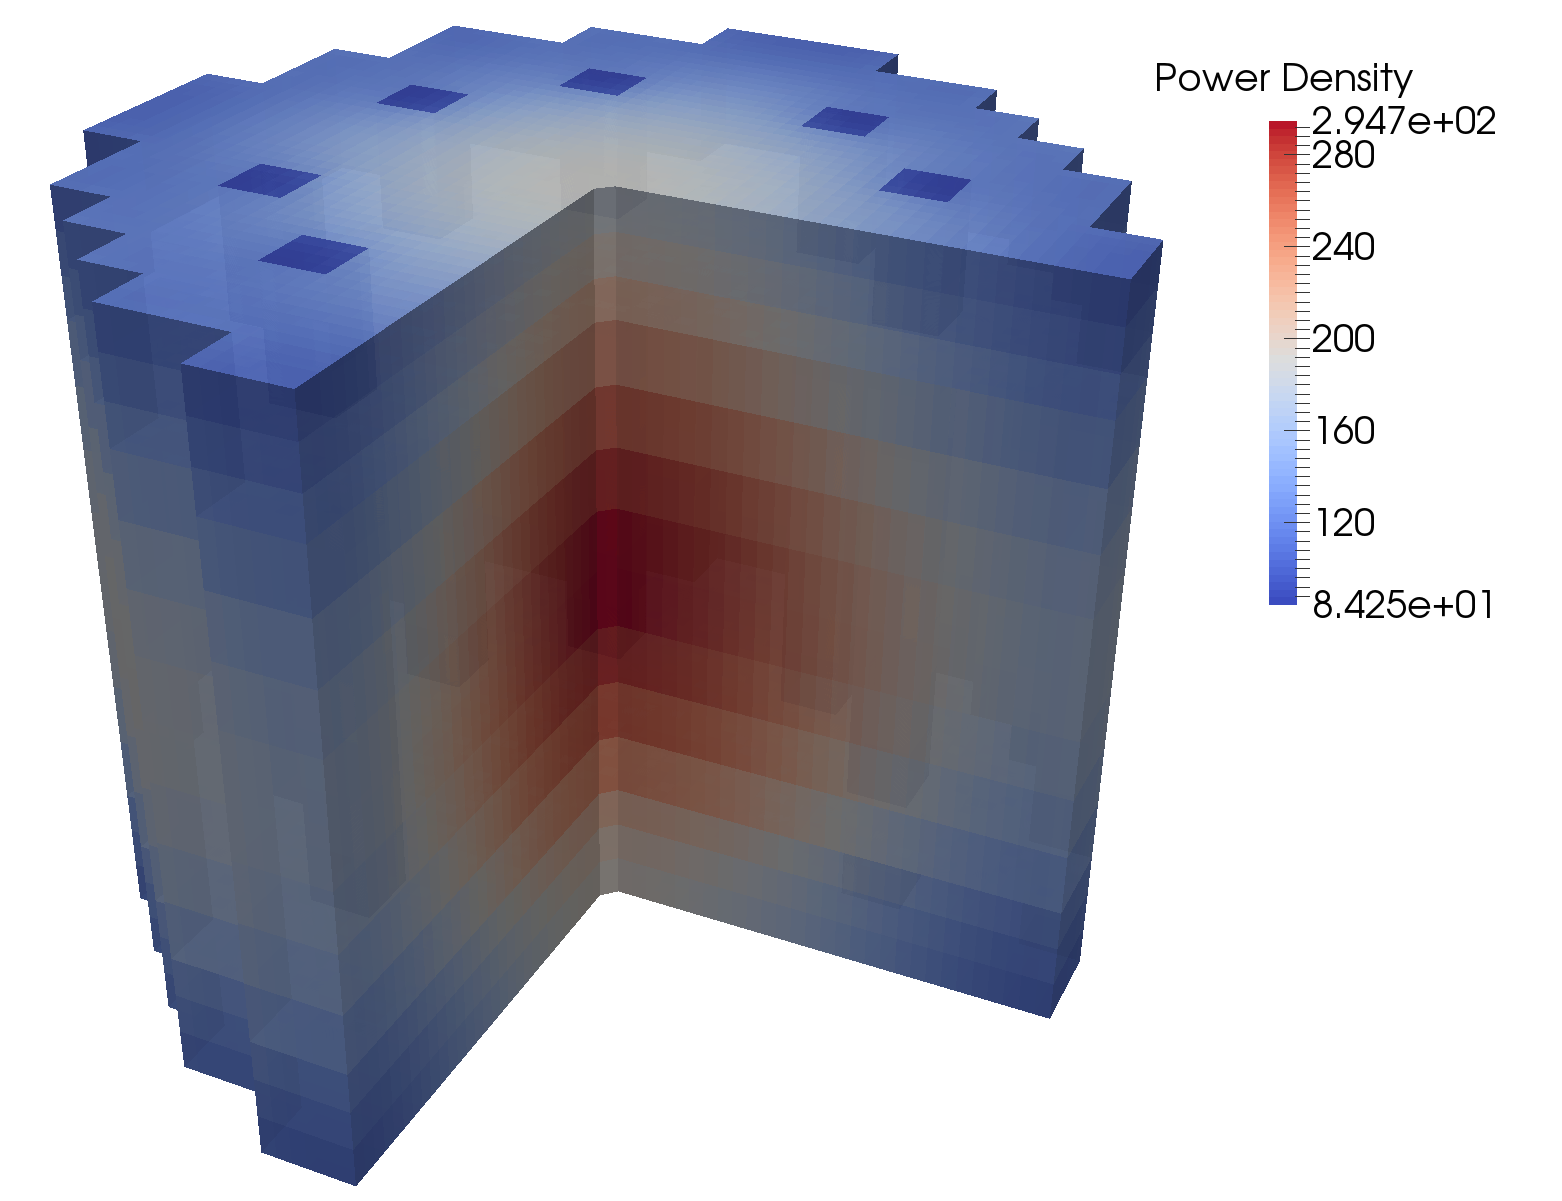
\includegraphics[width=\linewidth]{figures/Tran15_core2.png}
\end{figure}

\column{0.5\textwidth}
\begin{figure}
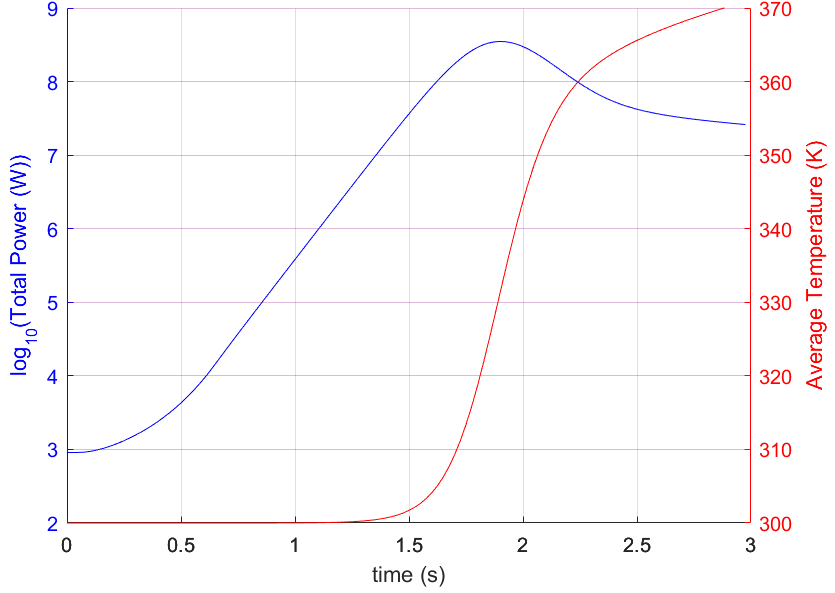
\includegraphics[width=\linewidth]{figures/Tran15_profile.png}
\end{figure}

\end{columns}
\end{frame}
%-------------------------------------------------------------------

%-------------------------------------------------------------------
\begin{frame}{Transient-15 Results}
\vspace{-3mm}

\begin{block}{Accuracy and Runtime}
\begin{center}
\resizebox{\linewidth}{!}{
\begin{tabular}{|l|ccc|}
\hline
Method & No. of Steps & \% Increase Runtime$^*$ & Max Power Error \\
\hline
Implicit Dis. 		& 300 &	---		&	7.875e-4	\\
IQS 				& 300 & -11.9\%	&	8.385e-5	\\
IQS (5 updates) 	& 300 &  49.7\%	&	3.687e-5	\\
IQS P-C 			& 300 &  -2.1\%	&	7.527e-4	\\
IQS P-C (5 updates) & 300 &  26.5\%	&	1.227e-4	\\
\hline
\end{tabular}
}
\end{center}
\vspace{-3mm}
$^*$ difference in runtime from implicit discretization 
\end{block}

\begin{block}{Dynamical Time Scale}
\begin{figure}
\includegraphics[height=1.5in]{figures/time_constant_tran15.png}
\end{figure}
\end{block}


\end{frame}
%-------------------------------------------------------------------

%-------------------------------------------------------------------
\begin{frame}{Transient-15 with Time Adaptation}

\begin{columns}

\column{.6\textwidth}
\begin{figure}
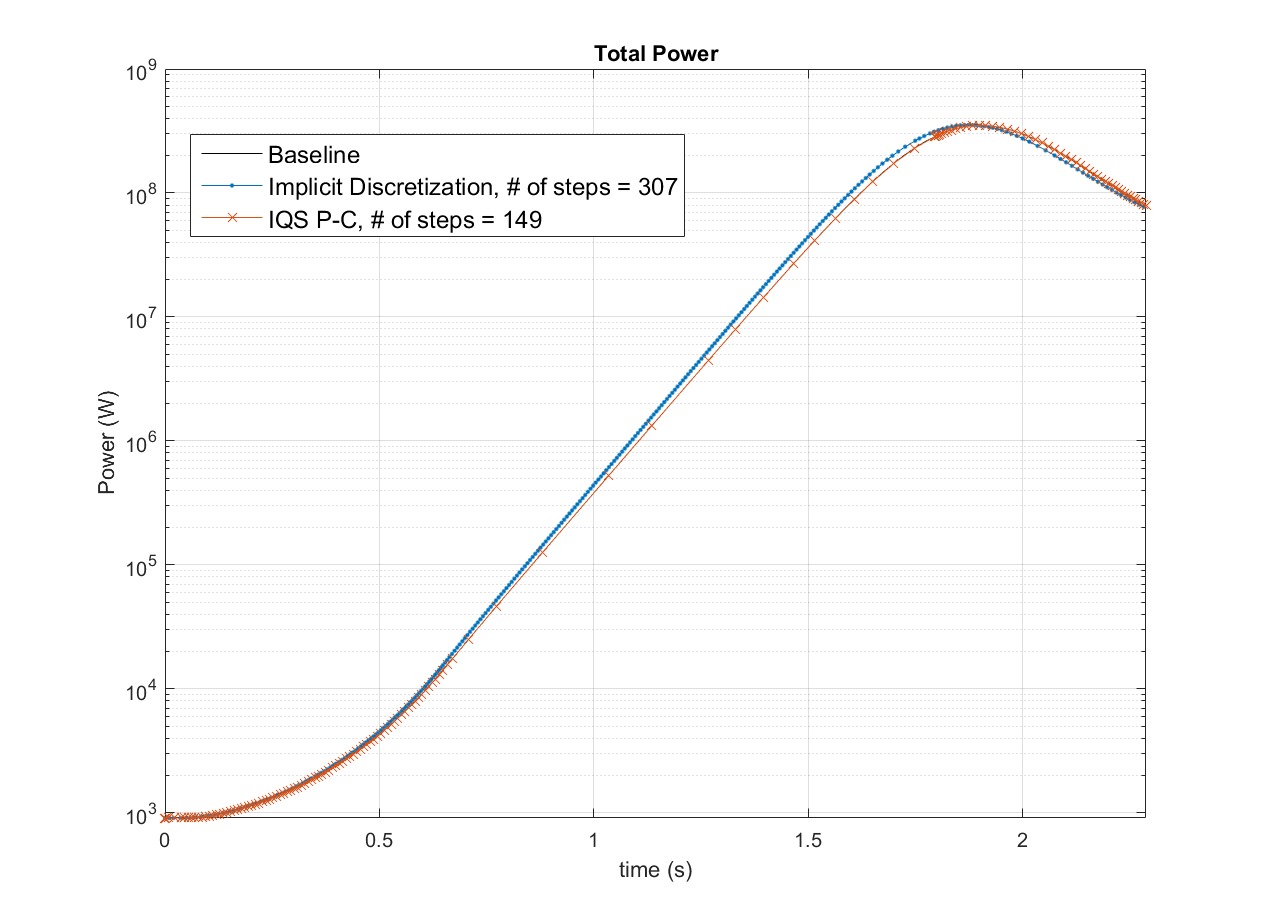
\includegraphics[width=\linewidth]{figures/Tran15_DT2.png}
\caption{TREAT Power Profile}
\end{figure}

\column{.6\textwidth}
\begin{figure}
\includegraphics[width=\linewidth]{figures/Tran15_DT2_peak.png}
\caption{TREAT Peak Power Profile}
\end{figure}

\end{columns}

\end{frame}
%-------------------------------------------------------------------

%%%%%%%%%%%%%%%%%%%%%%%%%%%%%%%%%%%%%%%%%%%%%%%%%%%%%%%%%%%%%%%%%%%%
\section{Conclusions}
%%%%%%%%%%%%%%%%%%%%%%%%%%%%%%%%%%%%%%%%%%%%%%%%%%%%%%%%%%%%%%%%%%%%

%-------------------------------------------------------------------
\begin{frame}{Conclusions}

\begin{block}{IQS Iteration}
IQS was testing with fixed point itertion used the following criteria:
\begin{enumerate}
\item $L^\infty$ norm of the change in shape between iterations
\item $L^2$ norm of the change in shape between iterations
\item Difference in reactivity between iterations
\item Difference in amplitude between iterations
\item IQS uniqueness consistency criteria
\end{enumerate}
\begin{itemize}
\item 1-4 had equivalent behavior
\item 5 required analytical integration of precursors for reasonable error convergence
\end{itemize}
\end{block}

\end{frame}
%-------------------------------------------------------------------

%-------------------------------------------------------------------
\begin{frame}{Conclusions (cont.)}

\begin{block}{IQS Time Step Error Convergence}
\begin{itemize}
\item Demonstrated proper convergence through order 4
\item Required higher order interpolation of PRKE parameters for higher order convergence
\item Effectiveness of error convergence demonstrated through time adaptation
\item Marginal improvement over implicit discretization for "difficult" 1D problem
\item Significant improvement for TWIGL and LRA
\end{itemize}
\end{block}

\begin{block}{IQS with Temperature Feedback}
\begin{itemize}
\item IQS was successfully implemented into the Rattlesnake/MOOSE framework
\item Added intermediate time scale loop for temperature
\item Incorporation of temperature into the quasi-static process significantly improved computational efficiency
\item Dynamical time scale analysis demonstrated proof-of-concept for variant time scales
\end{itemize}
\end{block}

\end{frame}
%-------------------------------------------------------------------


%-------------------------------------------------------------------
\begin{frame}{Recommendations for Future Research}

\begin{block}{Multiphysics}
Test IQS with other reactor physics, including:
\begin{itemize}
\item More complex temperature feedback
\item Thermal Hydraulics
\item Fuel Mechanics
\end{itemize}
\end{block}

\begin{block}{Transport}
Apply IQS to other transport models (other Rattlesnake action systems):
\begin{itemize}
\item DFEM-Diffusion
\item SAAF-Sn
\item SAAF-Pn
\item LS-Sn
\end{itemize}
\end{block}

\begin{block}{PJFNK}
\begin{itemize}
\item Investigate PJFNK iteration of IQS
\item Optimize IQS preconditioning
\end{itemize}
\end{block}

\end{frame}
%-------------------------------------------------------------------

%-------------------------------------------------------------------
\begin{frame}{Questions?}

\centering
\includegraphics[width=\linewidth,height=3in,keepaspectratio]{figures/question_mark.jpg}

\end{frame}
%-------------------------------------------------------------------

%-------------------------------------------------------------------
\begin{frame}

\begin{figure}
\includegraphics[height=0.5in]{figures/thank_you.png}
\end{figure}

\begin{figure}
\includegraphics[height=2.5in]{figures/nuclear_collage.png}
\hspace{5mm}
\includegraphics[height=2.5in]{figures/tamu_atom.jpg}
\end{figure}

\end{frame}
%-------------------------------------------------------------------

%%%%%%%%%%%%%%%%%%%%%%%%%%%%%%%%%%%%%%%%%%%%%%%%%%%%%%%%%%%%%%%%%%%%
\backupbegin
%%%%%%%%%%%%%%%%%%%%%%%%%%%%%%%%%%%%%%%%%%%%%%%%%%%%%%%%%%%%%%%%%%%%

%-------------------------------------------------------------------
\begin{frame}{Fixed-point iteration}
%\vspace{-10mm}

\begin{figure}
\includegraphics[height=1.3in]{figures/fixed_point.png}
\end{figure}
%\vspace{-10mm}
\begin{block}{IQS iteration approach}
\setlength{\leftmargini}{10mm}
\begin{itemize}
\item[\textit{Step 1:}] Compute the PRKE parameters at the end of the macro step using the last computed shape
\item[\textit{Step 2:}] Linearly interpolate the computed PRKE parameters over the macro step
\item[\textit{Step 3:}] Solve the PRKE on micro steps over the entire macro step
\item[\textit{Step 4:}] Solve the shape equation on the macro step using the computed values of $p$ and $dp/dt$.
\item[\textit{Step 5:}] Check if the shape solution has converged:
	\begin{itemize}
	\item \textit{No:} Repeat the same macro time step
	\item \textit{Yes:} Move on to the next macro time step
	\end{itemize}
\end{itemize}
\end{block}

\end{frame}
%-------------------------------------------------------------------

%-------------------------------------------------------------------
\begin{frame}{Fixed-point iteration programming logic}

\begin{figure}[!htpb]
\centering
\resizebox{!}{3in}{
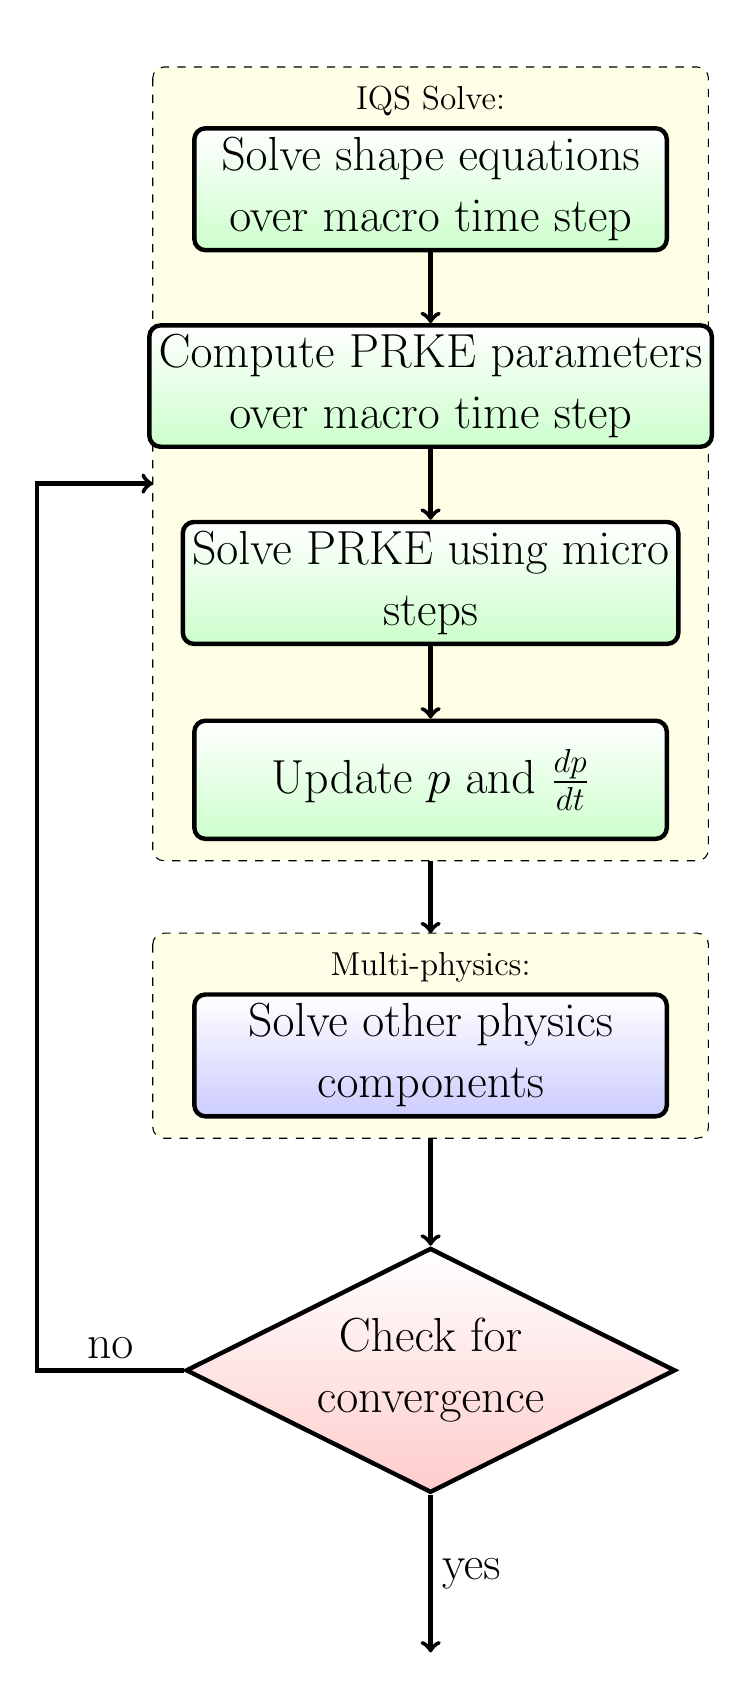
\begin{tikzpicture}[every node/.style = {font=\LARGE}]

\node[greenblock](p1) at (0,0) {Solve shape equations \\ over macro time step};
\node[greenblock](p2) at (0,-2.5) {Compute PRKE parameters \\ over macro time step};
\node[greenblock](p3) at (0,-5) {Solve PRKE using micro \\ steps};
\node[greenblock](p4) at (0,-7.5) {Update $p$ and $\frac{dp}{dt}$};
\node[blueblock2] (p5) at (0,-11) {Solve other physics \\ components};
\node[reddiamond] (check) at (0,-15) {Check for \\ convergence};
\node [above =0.1mm of p1] {\large{IQS Solve:}};
\node [above =0.1mm of p5] {\large{Multi-physics:}};

\tikzback{p1}{p1}{p4}{p4}{bk1}
\tikzback{p5}{p5}{p5}{p5}{bk2}

\draw[->,ultra thick](p1.south) -- (p2.north);
\draw[->,ultra thick](p2.south) -- (p3.north);
\draw[->,ultra thick](p3.south) -- (p4.north);
\draw [->,ultra thick] (p4.south)+(0,-0.25) -- node [above] {} (bk2-n);
\draw[->,ultra thick](p5.south)+(0,-0.25) -- (check.north);
%\draw[->,ultra thick](check.west) -- (-5,-15) -- node[above,sloped] {\large{no}}(-5,0) -- node[above] {}(bk1-w);
\draw[->,ultra thick](check.west) -- node[above,sloped] {\LARGE{no}} (-5,-15) |-  node[above] {}(bk1-w);
\draw[->,ultra thick](check.south) -- node[right] {\LARGE{yes}} ++(0,-2);

\end{tikzpicture}
}
\end{figure}

\end{frame}
%-------------------------------------------------------------------

%-------------------------------------------------------------------
\begin{frame}{Newton iteration}
\vspace{-3mm}
\begin{figure}
\includegraphics[height=1.1in]{figures/newton_iter.jpg}
\end{figure}
\vspace{-3mm}
\begin{block}{Jacobian-Free Newton-Krylov Method}
\bi
\item Newton system:
\be
J\delta\varphi = F(\varphi,p,t) - A(\varphi,p)\varphi \equiv -R(\varphi,p)
\ee
\item Where $J$ is the Jacobian and defined as:
\be
J_{ij}=\partial R_i/\partial\varphi_j
\ee
\item For IQS, the Jacobian is impossible to define so it must be approximated:
\be
J\delta\varphi\approx[R(\varphi+\epsilon\delta\varphi,p')-R(\varphi,p)]/\epsilon
\ee
\item The resulting system is solved using GMRES iteration
\ei
\end{block}

\end{frame}
%-------------------------------------------------------------------

%-------------------------------------------------------------------
\begin{frame}{Time Discretization Schemes}
\vspace{-3mm}

\begin{block}{General Equation Form}
\be 
IV\frac{\partial \varphi}{\partial t} = A\varphi+b
\ee
\end{block}
\vspace{-3mm}

\begin{block}{Theta Method}
\be
\varphi_{n+1} = (IV-\Delta t A_{n+1})^{-1}\left[\Delta t(1-\theta)(A_n\varphi_n+b_n) + \Delta t\theta b_{n+1} + IV\varphi_n\right]
\ee
\begin{itemize}
\item Implicit Euler: $\theta=1$ (First Order)
\item Explicit Euler: $\theta=0$ (First Order)
\item Crank-Nicolson: $\theta=1/2$ (Second Order)
\end{itemize}
\end{block}
\vspace{-3mm}

\begin{block}{Backward Difference Formula (BDF)}
\be 
\varphi_{n+1} = (IV-\Delta t A_{n+1})^{-1}\left[IV\sum_{j=1}^{k}\alpha_{j}^{k}\varphi_{n-(k-j)} + \Delta t \alpha_{k+1}^{k} b_{n+1}\right]
\ee
\centering
\begin{tabular}{c|lllll}
\hline
Order ($k$) & $\alpha_{1}^{k}$ & $\alpha_{2}^{k}$ & $\alpha_{3}^{k}$ & $\alpha_{4}^{k}$ & $\alpha_{5}^{k}$ \\
\hline
1 & 1 & 1 & & & \\
2 & -1/3 & 4/3 & 2/3 & & \\
3 & 2/11 & -9/11 & 18/11 & 6/11 & \\
4 & -3/25 & 16/25 & -36/25 & 48/25 & 12/25 \\
\hline
\end{tabular}
\end{block}

\end{frame}
%-------------------------------------------------------------------

%-------------------------------------------------------------------
\begin{frame}{Time Discretization Schemes (cont.)}

\begin{block}{Singly-Diagonally-Implicit Runge-Kutta (SDIRK)}
For a general differential equation $dy/dt=f(t,y)$:
\be
y_{n+1} = y_n + \Delta t\sum_{i=1}^s b_ik_i
\ee
\be 
k_i = f(t_n+c_i\Delta t, y_n+\Delta t \sum_{j=1}^{i} a_{ij}k_j)
\ee
\resizebox{\linewidth}{!}{
\begin{tabular}{cc}
Butcher Tableu: & SDIRK33: \\
\begin{tabular}{c|cccc}
$c_1$ & $a_{11}$ & &  & \\
'$c_2$ & $a_{21}$ & $a_{22}$ & & \\
$\vdots$ & $\vdots$ & $\vdots$ & $\ddots$ & \\
$c_s$ & $a_{s1}$ & $a_{s2}$ & $\ldots$ & $a_{ss}$\\
\hline
&$b_1$ & $b_2$ & $\ldots$ & $b_s$
\end{tabular}
&
\begin{tabular}{c|ccc}
$\lambda$ & $\lambda$ & & \\
$\frac{1}{2}(1+\lambda)$ & $\frac{1}{2}(1-\lambda)$ & $\lambda$ & \\
$1$ & $\frac{1}{4}(-1+16\lambda-6\lambda^2)$ & $\frac{1}{4}(5-20\lambda+6\lambda^2)$ & $\lambda$\\
\hline
 & $\frac{1}{4}(-1+16\lambda-6\lambda^2)$ & $\frac{1}{4}(5-20\lambda+6\lambda^2)$ & $\lambda$
\end{tabular} \\
 & Where $\lambda\approx0.4358665215$ satisfies $1-9\lambda+18\lambda^2-6\lambda^3=0$
\end{tabular}
}
\end{block}

\end{frame}
%-------------------------------------------------------------------

%-------------------------------------------------------------------
\begin{frame}{Time Step Error Convergence}
\vspace{-3mm}

\begin{figure}
\includegraphics[height=1.8in]{figures/gen_conv.png}
\end{figure}
\vspace{-3mm}

\begin{block}{}
\begin{itemize}
\item Validation through error convergence is vital for error quantification and time adaptation
\item Analysis involves:
\begin{enumerate}
\item Running simulation at variant time step sizes
\item Determining the error in power at time of interest based on baseline (very small time step) calculation
\item Using least-squares fit to determine the slope of error vs. $\Delta t$ on log scale
\end{enumerate}
\end{itemize}
\end{block}

\end{frame}
%-------------------------------------------------------------------

%-------------------------------------------------------------------
\begin{frame}{Time Adaptation Theory}

\begin{block}{Motivation}
\begin{itemize}
\item The concept of time adaptation is to have the behavior of some aspect of the evaluation determine the size of the time step.
\item The computational efficiency of IQS is best demonstrated when time adaptation is applied.
\item Step doubling adaptation was chosen because it is relatively simple and it utilizes the behavior of the solution to determine step size.
\end{itemize}
\end{block}

\begin{block}{Local Truncation Error}
We can estimate the local truncation error of the latest solve with a Taylor series expansion:
\be
\norm{LTE_n} = \Delta t_n^{p+1} \norm{\frac{\phi^{(p+1)}_{n}}{(p+1)!} + \Delta t_n \frac{\phi^{(p+2)}_{n}}{(p+2)!} + ...}
\ee
Where $p$ is the time discretization method's order and $\phi_n$ is the solution at time $ = t_n$. $\Delta t_n$ was the latest solves time step and $\Delta t_{n+1}$ is the next solves time step that has a desired error $\norm{LTE_{n+1}}$.  It can be
\end{block}

\end{frame}
%-------------------------------------------------------------------


%-------------------------------------------------------------------
\begin{frame}{Step Doubling Theory}

\begin{block}{New Step Size}
Using the definitions of the local errors:
\be
\Delta t_{n+1}^{p+1} \simeq \Delta t_{n}^{p+1} \tcm{\theta} \frac{\tcg{\norm{LTE_{n+1}}}}{\tcm{\norm{LTE_{n}}}}
\ee
Where $\tcm{\theta} \equiv 1 + O(\Delta t_n)$. $\tcg{\norm{LTE_{n+1}}}$ is some user defined relative error tolerance (\tcg{$e_{tol}$}) and \tcm{$e_n \equiv \frac{\theta}{\norm{LTE_{n}}}$} is a method's approximation to the last step's local error.  Therefore in practice:
\be
\Delta t_{new} = \Delta t_{old} \left[\frac{\tcg{e_{tol}}}{\tcm{e_n}}\right]^{1/(p+1)}
\ee
\end{block}

\begin{block}{Step Doubling}
Step doubling approximates the local error ($\tcg{e_n}$) by taking the difference in the local error of a solution with $\Delta t$ ($\phi_{\Delta t}$) and $\Delta t/2$ ($\phi_{\Delta t/2}$):
\be
e_n = \frac{\norm{\phi_{\Delta t/2} - \phi_{\Delta t}}}{\text{max}\left(\norm{\phi_{\Delta t/2}},\norm{\phi_{\Delta t}}\right)}
\ee
\end{block}

\end{frame}
%-------------------------------------------------------------------

%-------------------------------------------------------------------
\begin{frame}{MATLAB Kinetics Prototype Code (cont.)}

\begin{block}{Time Discretization Schemes}
\begin{itemize}
\item Embedded Rung-Kutta time adaptation with ode15s
\item Implicit Euler
\item First-fourth order BDF
\item Third order SDIRK (SDIRK33)
\end{itemize}
\end{block}

\begin{block}{IQS Process}
\begin{enumerate}
\item Intial steady-state eigenvalue evaluation
\item ode15s baseline calculation for error comparison
\item PRKE parameter calculation at macro steps
\item ode15s PRKE evaluation using interpolated PRKE parameters for \tcr{amplitude}
\item Build left- and right-hand-side system for \tcb{shape}
\item Evaluate \tcb{shape} using backslash operation
\item Iterate \tcr{amplitude} and \tcb{shape} until convergence
\item Evaluate precursors
\end{enumerate}
\end{block}

\end{frame}
%-------------------------------------------------------------------

%-------------------------------------------------------------------
\begin{frame}{Rattlesnake Structure}

\begin{figure}
\includegraphics[width=\linewidth,height=\textheight,keepaspectratio]{figures/rattlesnake.png}
\end{figure}

\end{frame}
%-------------------------------------------------------------------

%-------------------------------------------------------------------
\begin{frame}{IQS Implementation in Rattlesnake}

\begin{block}{IQS Components in Rattlesnake}
\begin{itemize}
\item IQS Executioner
	\begin{itemize}
	\item Convergence criteria for Picard iteration:
	\be
	Error_{IQS}=\left|\frac{\sum_{g=1}^G\left(\phi^{*g},\frac{1}{v^g}\varphi^{g,n}\right)}{\sum_{g=1}^G\left(\phi^{*g},\frac{1}{v^g}\varphi^{g,0}\right)}-1\right|
	\ee
	\item Evaluates PRKE using implicit Euler, Crank-Nicolson, or SDIRK33 with step doubling adaptation for $\frac{1}{p}\frac{dp}{dt}$ term
	\end{itemize}
\item PRKE Parameter Postprocessors
	\begin{itemize}
	\item Performs integrations for PRKE parameters
	\item Residuals from kernels are saved for $\rho-\bar{\beta}$ integration
	\end{itemize}
\item PRKE User Object
	\begin{itemize}
	\item Gathers postprocessor values
	\end{itemize}
\item IQS Removal Kernel
	\begin{itemize}
	\item Removal kernel for $\frac{1}{v^g}\frac{1}{p}\frac{dp}{dt}\varphi^g$ term
	\end{itemize}
\item Auxkernels
	\begin{itemize}
	\item Precursor auxkernel with analytical integration
	\item Temperature auxkernel with analytical integration
	\end{itemize}
\end{itemize}
\end{block}

\end{frame}
%-------------------------------------------------------------------

%-------------------------------------------------------------------
\begin{frame}{IQS Implementation in Rattlesnake (cont.)}
\vspace{-3mm}
\begin{block}{IQS Kernels}
\small
\begin{align*}
\frac{1}{v^g}\frac{\partial\varphi^g}{\partial t}=&\underbrace{\frac{\chi_p^g}{\keff} \sum_{g'=1}^G (1-\beta) \nu^{g'} \Sigma_f^{g'} \varphi^{g'}}_{Flux Kernel} + \underbrace{\sum_{g'\neq g}^G\Sigma_s^{g'\to g} \varphi^{g'}}_{Flux Kernel} - \underbrace{\left( -\div D^g \grad \right)\varphi^g}_{Flux Kernel} - \underbrace{\Sigma_r^g\varphi^g}_{Flux Kernel} \nonumber \\
& - \underbrace{\frac{1}{v^g} \boxed{\overbrace{\frac{1}{p}\frac{dp}{dt}}^{From Executioner}}\varphi^g}_{IQS Kernel}+\underbrace{\frac{1}{p}\sum_{i=1}^I\chi_{d,i}^g\lambda_iC_i}_{Modified Flux Kernel}
\end{align*}
\end{block}
\vspace{-2mm}

\begin{figure}
\resizebox{!}{1.5in}{
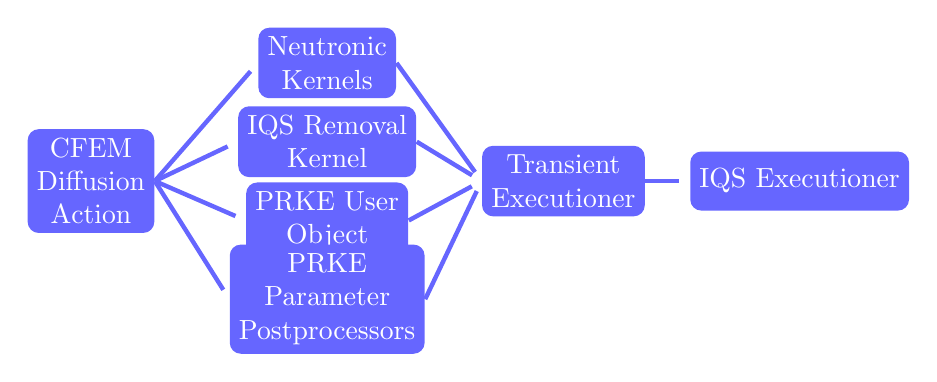
\begin{tikzpicture}[every node/.style = {shape          = rectangle, rounded corners, fill = blue!60, minimum width  = 1.5cm, minimum height = 0.75cm, align= center, text = white},blue edge/.style  = { -, ultra thick, blue!60, shorten >= 4pt}]
\node(0;0) at (-1,0) {CFEM \\ Diffusion \\ Action};
  \node(1;3)  at (2, 1.5) {Neutronic \\ Kernels};   
  \node(1;1)  at (2, 0.5) {IQS Removal \\ Kernel}; 
  \node(1;-1)  at (2,-0.5) {PRKE User \\ Object}; 
  \node(1;-3) at (2,-1.5) {PRKE \\ Parameter \\ Postprocessors}; 
     \node(2;0)  at (5,0) {Transient \\ Executioner};
     	\node(3;0)  at (8,0) {IQS Executioner};
\foreach \j in {-3,-1,1,3}
  { \draw[blue edge] (0;0.east) -- (1;\j.west); }
\foreach \j in {-3,-1,1,3}
  { \draw[blue edge] (1;\j.east) -- (2;0.west);} 
\draw[blue edge] (2;0.east) -- (3;0.west);         
\end{tikzpicture}
}
\end{figure}

\end{frame}
%-------------------------------------------------------------------

%-------------------------------------------------------------------
\begin{frame}{SDIRK Convergence Problems}

\begin{block}{Manufactured Solution}
\be 
\phi(x,t) = x(1-x)(1+t)^4 \qq 0 \leq x \leq 1
\ee
\be 
\frac{1}{v}\frac{\partial\phi}{\partial t} = \alpha\phi + \frac{\beta}{v}4(1+t)^3 + \gamma(1+t)^4
\ee
\end{block}

\begin{columns}

\column{.6\textwidth}
\begin{figure}
\includegraphics[width=\linewidth]{figures/sdirk_mms1.png}
\caption{SDIRK33 vs. BDF convergence with $v=1e5$}
\end{figure}

\column{.6\textwidth}
\begin{figure}
\includegraphics[width=\linewidth]{figures/sdirk_mms2.png}
\caption{SDIRK33 convergence with different velocities}
\end{figure}

\end{columns}

\end{frame}
%-------------------------------------------------------------------

%%%%%%%%%%%%%%%%%%%%%%%%%%%%%%%%%%%%%%%%%%%%%%%%%%%%%%%%%%%%%%%%%%%%
\backupend
%%%%%%%%%%%%%%%%%%%%%%%%%%%%%%%%%%%%%%%%%%%%%%%%%%%%%%%%%%%%%%%%%%%%

%************************************************

\end{document}